\documentclass{VUMIFPSkursinis}
\usepackage{algorithmicx}
\usepackage{algorithm}
\usepackage{algpseudocode}
\usepackage{amsfonts}
\usepackage{amsmath}
\usepackage{bm}
\usepackage{caption}
\usepackage{color}
\usepackage{float}
\usepackage{graphicx}
\usepackage{listings}
\usepackage{subfig}
\usepackage{wrapfig}
\usepackage[export]{adjustbox}
\usepackage{enumitem}
\usepackage{rotating}
\usepackage{hhline}
\usepackage{multirow}
\usepackage{tabularx}
\usepackage{array}
\usepackage{booktabs,calc}
\usepackage{indentfirst}
\setlength{\parindent}{1.5cm}
\usepackage{tabularx,colortbl}
\setitemize{noitemsep,topsep=0pt,parsep=0pt,partopsep=0pt}
\setenumerate{noitemsep,topsep=0pt,parsep=0pt,partopsep=0pt}
\usepackage[table]{xcolor}  
% Titulinio aprašas
\university{Vilniaus universitetas}
\faculty{Matematikos ir informatikos fakultetas}
\department{Programų sistemų katedra}
\papertype{Programų sistemų inžinerijos I-III laboratoriniai darbai}
\title{Darbo pasiūlymų valdymo sistema}
\titleineng{JOB OFFERS' MANAGEMENT SYSTEM}
\status{2 kurso 5 grupės studentai}
\author{Monika Čepulytė}
\secondauthor{Milda Jocaitė}
\thirdauthor{Vytautas Krivickas}
\fourthauthor{Mantas Naujokas}
% \secondauthor{Vardonis Pavardonis}   % Pridėti antrą autorių
\supervisor{dr. Vytautas Valaitis}
\date{Vilnius – \the\year}

% Nustatymai
% \setmainfont{Palemonas}   % Pakeisti teksto šriftą į Palemonas (turi būti įdiegtas sistemoje)
\bibliography{bibliografija}

\begin{document}
% PAKEISTA	
\maketitle
\cleardoublepage\pagenumbering{arabic}
\setcounter{page}{2}

\section*{ANOTACIJA}
Šis dokumentas sudarytas iš trijų dalių. Pirmoje dalyje pateikiama dalykinės srities analizė. Išorinėje verslo proceso analizėje identifikuojamos pagrindinės grėsmės ir galimybės. Vidinėje verslo proceso analizėje nustatomos verslo stiprybės ir silpnybės, kylančios iš paties verslo proceso. Dokumente taip pat pateikiamos verslo tobulinimo strategijos, nagrinėjamos galimybės įgyvendinti sistemą tiek technininiu požiūriu, tiek ir ekonominiu, pagrindžiant, ar projektas atsipirks. Antroje dalyje detaliai išdėstomi pagrindiniai darbo pasiūlymų valdymo sistemos reikalavimai. Pateikiama vartotojo interfeiso, funkcinių ir nefunkcinių programų sistemos reikalavimų specifikacija, kuria siekiama užtikrinti kuriamos programinės įrangos funkcionalumą bei poreikių atitikimą. Trečioje dalyje aprašoma kuriamos sistemos architektūra naudojant UML 4+1 požiūrių rinkinį. Žvelgiama į sistemą 5 skirtingais požiūriais. Loginis pjūvis skirtas parodyti sistemos funkcionalumą, aprašyti santykius tarp esybių. Užduočių pjūvyje pateiksime, kokias užduotis gali įgyvendinti vartotojas, kokie jų įgyvendimo scenarijai.  Kūrimo pjūvyje pateikiama, kaip susiję atskiri komponentai. Fiziniame pjūvyje parodoma, kaip sistema išdėstoma tinkle, kaip ji diegiama, kokia įranga naudojama. Procesų pjūvis pateikia dinaminį sistemos modelį: paaiškina sistemoje vykstančius procesus, parodo, kaip procesai komunikuoja, galimus sistemos darbo atvejus.

%TURINYS
\tableofcontents

\sectionnonum{ĮVADAS}
Darbo pasiūlymų valdymo sistema skirta tam, jog palengvintų darbo ieškančiųjų bei jį siūlančiųjų kasdienybę bei suteiktų įrankį, leidžiantį darbuotojams greitai ir paprastai rasti patikimus, gerai įvertintus darbdavių pasiūlymus, o pastariesiems - atsakingų darbuotojų.
\newline
\newline
\textbf{Dalykinė sritis}

Skelbimai.
\newline
\newline
\textbf{Probleminė sritis}

„Workly" suteiktų galimybę greitai ir paprastai ieškoti dominančių darbo skelbimų. Darbai būtų filtruojami pagal įvairius naudotojo pageidaujamus kriterijus: vietovę, trukmę, veiklos pobūdį, užmokestį. Pagrindinis programėlės išskirtinumas, leidžiantis užpildyti dar gana neišnaudotą verslo nišą - trumpi, neterminuoti ir lengvai pasiekiami darbo skelbimai. 
\newline
\newline
\textbf{Naudoti dokumentai}
Dokumentas parengtas pagal kursinio darbo reikalavimus (žr. Literatūros sąrašas 2) naudotojant Latex programą ir jau sukurtus šabonus (žr. Literatūros sąrašas 1).
\newline
\newline
\textbf{Darbo pagrindas}
Dokumentas parengtas kaip Programų sistemų inžinerijos I-III laboratoriniai darbai.
\newpage
\section{KURIAMO VERSLO PROCESO ANALIZĖ}
Šiame skyriuje pateikiama kuriamo verslo proceso išorinė analizė, vidinė analizė. Padarytos išvados pateikiamos SSGG modelio principu. Taip pat pateikiamii sistemos panaudojimo scenarijai, verslo tobulinimo strategijos ir įgyvendinamumo bei naudos analizė.
\subsection{VERSLO PROCESO APRAŠAS}
Programos klientai esti dviejų tipų: darbuotojai ir darbdaviai (nors nėra apribojimų klientui būti tiek darbdaviu, tiek darbuotoju). Visų pirma, apsilankęs mūsų pulapyje (jei dar nėra to padaręs anksčiau) darbdavys privalo užsiregistruoti (prisijungti). Tik autentifikuoti vartotojai turi priėjimą prie esminės, programos pagrindinį funkcionalumą įgyvendinačios skilties Darbai. Čia galima peržvelgti esančių skelbimų sąrašą bei įkelti/redaguoti naujus darbo pasiūlymus. Įkėlęs skelbimą, darbdavys laukia, kol su juo susisieks interesantai. Galimas ir kitas scenarijus, kuomet, pasinaudojęs Top vartotojų skiltimi, darbdavys aktyviai ieško darbuotojų. Taip pat jam suteikiama galimybė reitinguoti ir rašyti atsiliepimus apie darbuotojus. Taip užtikrinamas programos siūlomos paslaugos kokybiškumas bei kitiems darbdaviams suteikiamos rekomendacijos, padėsiančios išsirinkti geriausius darbuotojus. Darbdavys taip pat gali peržiūrėti savo įkeltus darbo pasiūlymus, juos ištrinti ar redaguoti.

	Kitas klientų tipas - darbuotojas - pirmą kartą apsilankęs mūsų puslapyje taip pat privalo užsiregistruoti (tolimesnių apsilankymų metu pakanka tik prisijungimo). Po autentifikavimo, jam pasiekiamas pagrindinis programos resursas - darbo sklelbimų sąrašas. Čia, pasinaudojęs atlyginimo, trukmės, srities ir kitais filtrais, jis gali gauti dominančio pasiūlymo kūrėjo kontaktinius duomenis. Sutaręs dėl darbo atlikimo ir jį atlikęs, vartotojas gali palikti atsliepimą bei įvertinti darbdavį priskirdamas jam reitingą. Šie įvertinimai gerai matomi Top skiltyje, kurioje darbuotojas gali pasitikrinti prieš priimdamas darbo pasiūlymą.  Taip suteikiamas stimulas stengtis ne tik darbuotojams, bet ir darbdaviams. Kartu užtikrinamas ir mūsų programos siūlomos paslaugos. Darbuotojas gali susidaryti dominančių darbų sąrašą, kuriuos galės peržiūrėti bet kuriuo metu. Taip suteikiama darbuotojui galimybė greičiau susirasti prieš tai jam tinkantį darbo pasiūlymų.

Darbų valdymo sistemą prižiūri sistemos administratorius. Jis gali ištrinti darbuotoją ar darbdavių, jei jis pažeidžia sistemos naudojimosi sąlygas. Administratorius taip pat prižiūri, kad sistemoje nebūtų netaisyklingų darbo pasiūlymų (neatitinkančių realybės). 
\newpage

\subsection{IŠORINĖ ANALIZĖ}
1 skyriuje pateikiama kuriamo verslo proceso išorinė analizė. Jos metu išsiaiškinami ištekliai reikalingi pradėti verslą, kuriamos aplikacijos teikiami rezultatai ir išanalizuojama rinkoje esanti situacija. Nustačius rinkos esančius ir potencialius konkurentus įvertinama situacija, išanalizuojamos neišnaudotos galimybės. Šia analize taip pat išryškinamos kuriamo verslo grėsmės ir problemos.
\subsubsection{Įeigos, išeigos, įvaizdžio ir reguliavimo analizė}
Šiame skyriuje aprašoma kuriamo verslo proceso įeiga, išeiga, reguliavimas ir įvaizdis. Įeigoje aptariami pagrindiniai naudojami ištekliai, tuo tarpu išeigoje pagrindiniai veiklos rezultatai. Reguliavimo dalyje aptariama, kokias įstatymais, teisės aktais yra reguliuojamas verslo procesas. Kuriamą sistemą vertina išorinės grupės, todėl įvaizdžio dalyje aprašoma, koks išorinis vertinimas yra svarbus. 
\begin{figure}[H]
\centering
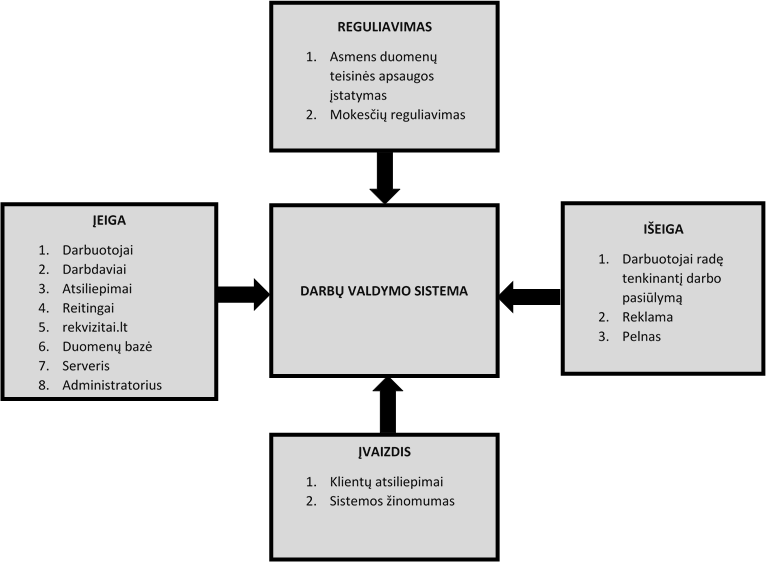
\includegraphics[width=\linewidth]{img/isorine2.png}
\caption{Įeigos, išeigos, įvaizdžio ir reguliavimo analizės diagrama}
\end{figure}
1 Lentelėje pateikiami įeigos, išeigos, reguliavimo ir įvaizdžio svarbiausi vertinimo kriteriai, jų matavimo vienetai. Nustatoma kritinė vertė, esama vertė ir siekiama vertė. Tai padeda nustatyti, ar tam tikras vertinimo kriterijus atitinka normas.
\begin{table}[H]
\caption{Vertinimo kriterijai, jų matavimo vienetai. Esama, siekiama ir kritinė vertės.}
\centering
\normalsize
\begin{tabular}{|p{0.6cm}|p{6cm}|p{3cm}|p{1.6cm}|p{1.5cm}|}
\hline
\rowcolor{gray!40}

\multicolumn{1}{|m{0.6cm}|}{\textbf{NR.}}&\multicolumn{1}{m{6cm}|}{\textbf{Vertinimo kriterijus}}&\multicolumn{1}{m{3cm}|}{\textbf{Vertinimo matas}}&\multicolumn{1}{m{1.6cm}|}{\textbf{Siekiama vertė}}&\multicolumn{1}{m{1.5cm}|}{\textbf{Kritinė vertė}}\\ \hline

\rowcolor{gray!10}
\multicolumn{5}{|l|}{\textbf{ĮEIGA}} \\ \hline

\multicolumn{5}{|l|}{\textbf{Darbuotojai}} \\ \hline

\multicolumn{1}{|m{0.6cm}|}{1.}&\multicolumn{1}{m{6cm}|}{Naujų užsiregistravusių darbuotojų skaičius per mėnesį.}&\multicolumn{1}{m{3cm}|}{Žmonių skaičius}&\multicolumn{1}{m{1.6cm}|}{200}&\multicolumn{1}{m{1.5cm}|}{70}\\ \hline

\multicolumn{1}{|m{0.6cm}|}{2.}&\multicolumn{1}{m{6cm}|}{Aktyvių darbutojų skaičius (peržiūri darbo pasiūlymus, rašo atsiliepimus, reitinguoja).}&\multicolumn{1}{m{3cm}|}{Procentas nuo visų darbuotojų}&\multicolumn{1}{m{1.6cm}|}{65}&\multicolumn{1}{m{1.5cm}|}{20}\\ \hline

\multicolumn{5}{|l|}{\textbf{Darbdaviai}} \\ \hline

\multicolumn{1}{|m{0.6cm}|}{3.}&\multicolumn{1}{m{6cm}|}{Naujų užsiregistravusių darbdavių skaičius per mėnesį.}&\multicolumn{1}{m{3cm}|}{Žmonių skaičius}&\multicolumn{1}{m{1.6cm}|}{200}&\multicolumn{1}{m{1.5cm}|}{70}\\ \hline

\multicolumn{1}{|m{0.6cm}|}{4.}&\multicolumn{1}{m{6cm}|}{Naujų pateiktų darbo pasiūlymų skaičius per mėnesį.}&\multicolumn{1}{m{3cm}|}{Darbo pasiūlymų skaičius}&\multicolumn{1}{m{1.6cm}|}{300}&\multicolumn{1}{m{1.5cm}|}{100}\\ \hline

\multicolumn{1}{|m{0.6cm}|}{5.}&\multicolumn{1}{m{6cm}|}{Dominančių darbo pasiūlymų skaičius.}&\multicolumn{1}{m{3cm}|}{Procentas nuo visų darbo pasiūlymų}&\multicolumn{1}{m{1.6cm}|}{80}&\multicolumn{1}{m{1.5cm}|}{30}\\ \hline

\multicolumn{1}{|m{0.6cm}|}{6.}&\multicolumn{1}{m{6cm}|}{Aktyvių darbdavių skaičius (pateikia darbo pasiūlymus, rašo atsiliepimus, reitinguoja).}&\multicolumn{1}{m{3cm}|}{Procentas nuo visų darbdavių}&\multicolumn{1}{m{1.6cm}|}{70}&\multicolumn{1}{m{1.5cm}|}{40}\\ \hline

\multicolumn{1}{|m{0.6cm}|}{7.}&\multicolumn{1}{m{6cm}|}{Peržiūrėtų darbo pasiūlymų skaičius.}&\multicolumn{1}{m{3cm}|}{Procentas nuo visų darbdavių}&\multicolumn{1}{m{1.6cm}|}{70}&\multicolumn{1}{m{1.5cm}|}{35}\\ \hline

\multicolumn{1}{|m{0.6cm}|}{8.}&\multicolumn{1}{m{6cm}|}{Pateiktų VIP darbo pasiūlymų skaičius per mėnesį (būti sąraše vieną dieną).}&\multicolumn{1}{m{3cm}|}{Darbo pasiūlymų skaičius}&\multicolumn{1}{m{1.6cm}|}{800}&\multicolumn{1}{m{1.5cm}|}{200}\\ \hline

\multicolumn{5}{|l|}{\textbf{Atsiliepimai}} \\ \hline

\multicolumn{1}{|m{0.6cm}|}{9.}&\multicolumn{1}{m{6cm}|}{Naujų atsiliepimų apie naudotojus skaičius per mėnesį}&\multicolumn{1}{m{3cm}|}{Atsiliepimų skaičius}&\multicolumn{1}{m{1.6cm}|}{400}&\multicolumn{1}{m{1.5cm}|}{100}\\ \hline

\multicolumn{1}{|m{0.6cm}|}{10.}&\multicolumn{1}{m{6cm}|}{Naudotojų skaičius, kurie turi atsiliepimus.}&\multicolumn{1}{m{3cm}|}{Procentas nuo visų naudotojų}&\multicolumn{1}{m{1.6cm}|}{70}&\multicolumn{1}{m{1.5cm}|}{30}\\ \hline

\multicolumn{5}{|l|}{\textbf{Reitingai}} \\ \hline

\multicolumn{1}{|m{0.6cm}|}{11.}&\multicolumn{1}{m{6cm}|}{Naudotojų skaičius, kurie turi reitingus.}&\multicolumn{1}{m{3cm}|}{Procentas nuo visų naudotojų}&\multicolumn{1}{m{1.6cm}|}{60}&\multicolumn{1}{m{1.5cm}|}{30}\\ \hline

\end{tabular}
\end{table}

\begin{table}[H]
\centering
\normalsize
\begin{tabular}{|p{0.6cm}|p{6cm}|p{2cm}|p{1.4cm}|p{1.6cm}|p{1.5cm}|}
\hline
\rowcolor{gray!40}

\multicolumn{1}{|m{0.6cm}|}{\textbf{NR.}}&\multicolumn{1}{m{6cm}|}{\textbf{Vertinimo kriterijus}}&\multicolumn{1}{m{3cm}|}{\textbf{Vertinimo matas}}&\multicolumn{1}{m{1.6cm}|}{\textbf{Siekiama vertė}}&\multicolumn{1}{m{1.5cm}|}{\textbf{Kritinė vertė}}\\ \hline

\multicolumn{1}{|m{0.6cm}|}{12.}&\multicolumn{1}{m{6cm}|}{Pateiktų reitingų skaičius per mėnesį.}&\multicolumn{1}{m{3cm}|}{Procentas nuo visų naudotojų}&\multicolumn{1}{m{1.6cm}|}{50}&\multicolumn{1}{m{1.5cm}|}{10}\\ \hline

\multicolumn{5}{|l|}{\textbf{rekvizitai.lt reitingai}} \\ \hline

\multicolumn{1}{|m{0.6cm}|}{13.}&\multicolumn{1}{m{6cm}|}{Naudotojų skaičius, kurie turi rekvizitai.lt reitingą}&\multicolumn{1}{m{3cm}|}{Procentas nuo visų naudotojų}&\multicolumn{1}{m{1.6cm}|}{40}&\multicolumn{1}{m{1.5cm}|}{10}\\ \hline

\multicolumn{5}{|l|}{\textbf{Duomenų bazė}} \\ \hline

\multicolumn{1}{|m{0.6cm}|}{14.}&\multicolumn{1}{m{6cm}|}{Duomenų bazės talpa.}&\multicolumn{1}{m{3cm}|}{Talpa GB}&\multicolumn{1}{m{1.6cm}|}{50}&\multicolumn{1}{m{1.5cm}|}{20}\\ \hline

\multicolumn{5}{|l|}{\textbf{Serveris}} \\ \hline

\multicolumn{1}{|m{0.6cm}|}{15.}&\multicolumn{1}{m{6cm}|}{Vidutinis užklausos apdorojimo laikas.}&\multicolumn{1}{m{3cm}|}{Sekundės}&\multicolumn{1}{m{1.6cm}|}{1}&\multicolumn{1}{m{1.5cm}|}{5}\\ \hline

\multicolumn{5}{|l|}{\textbf{Administratorius}} \\ \hline

\multicolumn{1}{|m{0.6cm}|}{16.}&\multicolumn{1}{m{6cm}|}{Pašalintų naudotojų skaičius per mėnesį.}&\multicolumn{1}{m{3cm}|}{Naudotojų skaičius}&\multicolumn{1}{m{1.6cm}|}{0}&\multicolumn{1}{m{1.5cm}|}{30}\\ \hline

\multicolumn{1}{|m{0.6cm}|}{17.}&\multicolumn{1}{m{6cm}|}{Pašalintų darbo pasiūlymų skaičius per mėnesį.}&\multicolumn{1}{m{3cm}|}{Darbo pasiūlymų skaičius}&\multicolumn{1}{m{1.6cm}|}{0}&\multicolumn{1}{m{1.5cm}|}{30}\\ \hline

\rowcolor{gray!10}
\multicolumn{5}{|l|}{\textbf{IŠEIGA}} \\ \hline

\multicolumn{1}{|m{0.6cm}|}{18.}&\multicolumn{1}{m{6cm}|}{Darbuotojai radę dominanatį darbo pasiūlymą.}&\multicolumn{1}{m{3cm}|}{Peržiūrėtų kontaktų skaičius per mėnesį}&\multicolumn{1}{m{1.6cm}|}{60}&\multicolumn{1}{m{1.5cm}|}{20}\\ \hline

\rowcolor{gray!10}
\multicolumn{5}{|l|}{\textbf{ĮVAIZDIS}} \\ \hline

\multicolumn{1}{|m{0.6cm}|}{19.}&\multicolumn{1}{m{6cm}|}{Facebook naujų „like“ skaičius per mėnesį.}&\multicolumn{1}{m{3cm}|}{„Like“ skaičiusį}&\multicolumn{1}{m{1.6cm}|}{50}&\multicolumn{1}{m{1.5cm}|}{20}\\ \hline

\multicolumn{1}{|m{0.6cm}|}{20.}&\multicolumn{1}{m{6cm}|}{Strapsnių apie sistemą žinasklaidoje skaičius per metus}&\multicolumn{1}{m{3cm}|}{Straipsnių skaičius}&\multicolumn{1}{m{1.6cm}|}{3}&\multicolumn{1}{m{1.5cm}|}{1}\\ \hline

\multicolumn{1}{|m{0.6cm}|}{21.}&\multicolumn{1}{m{6cm}|}{Teigiamų klientų atsiliepimų apie sistemą skaičius.}&\multicolumn{1}{m{3cm}|}{Procentas nuo visų atsiliepimų}&\multicolumn{1}{m{1.6cm}|}{80}&\multicolumn{1}{m{1.5cm}|}{50}\\ \hline

\rowcolor{gray!10}
\multicolumn{5}{|l|}{\textbf{REGULIAVIMAS}} \\ \hline

\multicolumn{1}{|m{0.6cm}|}{22.}&\multicolumn{1}{m{6cm}|}{Asmens duomenų teisinės apsaugos įstatymo pažeidimų per metus.}&\multicolumn{1}{m{3cm}|}{Pažeidimų skaičius}&\multicolumn{1}{m{1.6cm}|}{0}&\multicolumn{1}{m{1.5cm}|}{0}\\ \hline

\multicolumn{1}{|m{0.6cm}|}{23.}&\multicolumn{1}{m{6cm}|}{Mokesčių mokėjimo pažeidimų per metus.}&\multicolumn{1}{m{3cm}|}{Pažeidimų skaičius}&\multicolumn{1}{m{1.6cm}|}{0}&\multicolumn{1}{m{1.5cm}|}{0}\\ \hline

\end{tabular}
\end{table}

\subsubsection{Išorinė analizė pagal modelį „5 porterio jėgos"}
Taikant penkių Porterio jėgų metodą yra stebimi šie veiksniai: potencialūs konkurentai, konkurencija rinkos segmente, tiekėjai, prekės pakaitalai ir pirkėjai.
\begin{figure}[H]
\centering
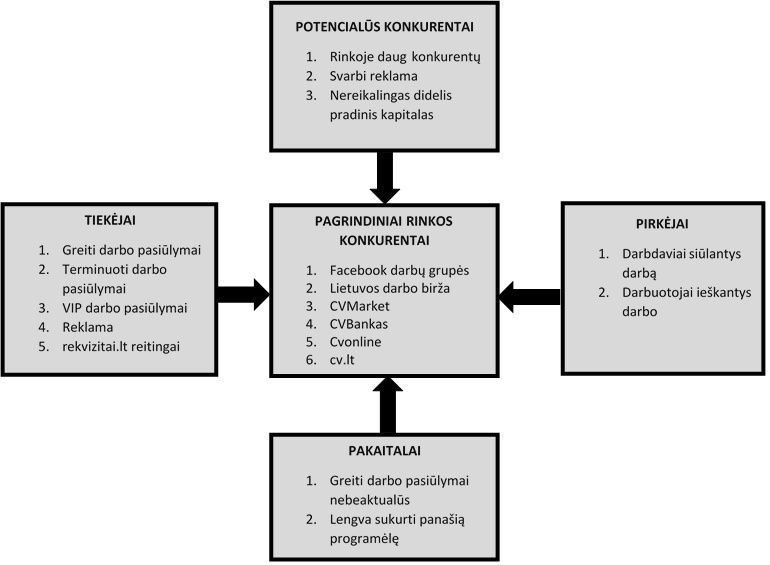
\includegraphics[width=\linewidth]{img/isorine1.png}
\caption{Analizės pagal modelį „5 porterio jėgos" diagrama}
\end{figure}
\paragraph{Potencialūs konkurentai}
Rinkoje yra daug sistemų, kuriuos pateikia darbdavių siūlomus darbo pasiūlymus, todėl naujiems konkurentams į rinką įeiti nėra lengva. Pagrindinė sėkmingo verslo proceso sąlyga – sistemos žinomumas.  Naujai susikūrusi sistema turi pritraukti darbuotojus ir darbdavius, išreklamuoti kuriamą produktą. Tačiau atsirasti potencialiems konkurentams padeda aplinkybė, kad nėra reikalingas didelis pradinis kapitalas.
\paragraph{Pagrindiniai rinkos konkurentai}
Rinkoje yra daug sistemų, kurios pateikia darbuotojų siūlomus darbo pasiūlymus, o darbdaviai suteikia galimybę peržiūrėti darbo pasiūlymus ir susisiekti su darbdaviu. Aptarsime pagirndinius (populiariausius) rinkoje egzistuojančius dalyvius: Facebook darbų grupės, Lietuvos darbo birža, CVMarket, CVBankas, CVonline, cv.lt. Pagrindinis mūsų kuriamo verslo konkurentas yra Facebook darbų grupės.  Kaip ir mūsų sistemoje, joje žmonės vieni kitiems siūlo laikinus, netermituotus darbo pasiūlymus. Šios sistemos didžiausi trūkumai sudėtinga paieška, nėra galimybės rūšiuoti, rikiuoti duomenis ir yra daug skirtingų grupių (duomenys nėra vienoje vietoje). Darbdavio duomenys dažniausiai nėra pateikiami automatiškai – juos galima gauti klausiant asmenine žinute. Taip pat reikia prisijungti prie grupės, sulaukti grupės administratoriaus patvirtinimo. 2-6 rinkos konkurentai specializuojasi į terminuotus, ilgus darbo pasiūlymus. Dažniausiai darbai yra siūlomi įmonių, norint priimti darbo pasiūlymą yra pasirašoma darbo sutartis.
\paragraph{Tiekėjai}
Pagrindinis mūsų kuriamo verslo proceso tiekėjas – darbdavių siūlomi darbo pasiūlymai. Sistemoje svarbiausi yra trumpi darbo pasiūlymai, bet taip pat sudaroma galimybė pateikti ir ilgus (terminuotus) darbo pasiūlymus. Mūsų sistema yra priklausoma nuo šio tiekėjo, nėra galimybės jį pakeisti. Kitas tiekėjas VIP darbo pasiūlymai – mokami darbo skelbimai, kurie yra rodomi atskiroje, išskirtoje skiltyje. Šis tiekėjas pasirinktas, nes daugelis darbų valdymo sistemų įgyvendina VIP skelbimus (pvz: cvmarket.lt). Dar vienas tiekėjas reklamos agentūros. Mūsų kuriamai sistemai svarbi reklama, todėl jų paslaugos bus reikalingos. Taip pat naudojami rekvizitai.lt surinkti duomenys. Darbdavio reitingas nustatomas atsižvelgiant į rekvizitai.lt turimą reitingą. Šis tiekėjas pasirinktas, nes žmonės pasitinki svetainės rekvizitai.lt pateikiamais reitingais.
\paragraph{Pirkėjai}
Kaip ir kiekvienos darbų valdymo sistemos, pagrindiniai pirkėjai yra darbdaviai ir darbuotojai. Darbdaviai yra suinteresuoti sistema, nes jiems reikalingas darbuotojas, tuo tarpu darbuotojas ieško darbo. Be šių dviejų pirkėjų sistema negali egzistuoti. Sistema taip pat talpins reklamą, todėl dar viena prikėjų rūšis yra klientai norintys patalpinti savo reklamą.
\paragraph{Pakaitalai}Greiti darbo pasiūlymai tampa vis aktualesni, todėl yra tik maža tikimybė, kad jie išnyks arba juos pakeis kas nors kitas. Tačiau mūsų kuriama aplikacija nėra sudėtinga, todėl gali atsirasti kitų panašių (atliekančių tas pačias funkcijas) aplikacijų.

\subsubsection{Grėsmės ir galimybės}

\paragraph{Grėsmės}
Kuriamas verslas procesas yra priklausomas nuo dviejų pagrindinių įvesčių - darbuotojų ir darbdavių. Jų skaičius ir aktyvumas lemia kuriamos programos sėkmę. Sėkmingam kuriamo verslo proceso egzistavimui turi įtakos reitingų ir atsiliepimų skaičius bei kokybė. Žmonių pasitikėjimą sistema padidintų objektyvūs reitingai ir atsiliepimai. Tačiau tai užtikrinti yra sudėtinga. Darbo valdymo sistemai kol kas trūksta žinomumo, todėl turi būti skiriamas didelis dėmesys reklamai socialiniuose tinkluose ir žiniasklaidoje. Verslo procesas renka asmeninius žmonių duomenis, todėl reikės pasirūpinti tinkamu duomenų saugojimu. Rinkoje jau egzistuoja panašių darbo valdymo sistemų, todėl konkurencija yra gana didelė. Taip pat verslo procesas nėra sudėtingas, todėl gali atsirasti naujų konkurentų.
\paragraph{Galimybės}
Rinkoje jau egzistuojančios darbo valdymo sistemos turi trūkumų (neefektyvi paieška, darbo pasiūlymai nėra vienoje vietoje, siūlomi ilgi (terminuoti) darbo pasiūlymai), todėl kuriama sistema gali juos išnaudoti, tapti patogesnė naudotojui. Sistema naudos reitingų ir atsiliepimų sistemą - konkurentų sistemos čios funkcijos neturi, todėl tai gali padėti pritraukti naujų darbuotojų ir darbdavių. Sistema suteiks galimybę turėti VIP pasiūlymus, kaip ir daugelis rinkoje jau egzistuojančių sistemų. Sistema taip galėtų suteikti automatinį apmokėjimą darbuotojui tinkamai atlikus darbą. Dar viena darbų valdymo sistemos galimybė automatiškai skambinti darbuotojui/darbdaviui vienu mygtuko paspaudimu, nes daugelis modernių aplikacijų turi šią funkciją. Sistema taip pat turėtų suteikti darbo pasiūlymų rūšiavimą pagal dabartinę vietą, tai būtų didelis privalumas, nes daugelis darbų valdymo sistemų šios funkcijos neturi.
\newpage
\subsection{VIDINĖ ANALIZĖ}
Toliau pateikiama keliais aspektais atlikta vidinė verslo proceso analizė, kuria siekiama nustatyti nagrinėjamo verslo stiprybes ir silpnybes, kylančias iš verslo proceso.

\subsubsection{Dalykinės srities statinė struktūra}
Toliau pateikiama dalykinės srities statinės struktūros UML diagrama. Joje matomos pagrindinės esybės bei jų tarpusavio sąveika. Klientai esti dviejų tipų: darbuotojai ir darbdaviai (nors nėra apribojimų klientui būti tiek darbdaviu, tiek darbuotoju). Visų pirma, darbdavys privalo užpildyti registracijos formą. Tik po to vartotojai gauna prieigą prie darbo skelbimų sąrašo. Čia galima peržvelgti ne tik esančių skelbimų sąrašą bet ir įkelti/redaguoti naujus darbo pasiūlymus. Įkėlęs skelbimą, darbdavys laukia, kol su juo susisieks interesantai. Galimas ir kitas scenarijus, kuomet, pasinaudojęs darbdavys aktyviai ieško darbuotojų. Taip pat jam suteikiama galimybė reitinguoti ir rašyti atsiliepimus apie darbuotojus. Taip užtikrinamas programos siūlomos paslaugos kokybiškumas bei kitiems darbdaviams suteikiamos rekomendacijos, padėsiančios išsirinkti geriausius darbuotojus. Kitas klientų tipas - darbuotojas - taip pat privalo užpildyti registracijos formą. Tik po šio žingsnio jam pasiekiamas pagrindinis resursas - darbo sklelbimų sąrašas. Čia, pasinaudojęs atlyginimo, trukmės, srities ir kitais filtrais, paieška, jis gali gauti dominančio pasiūlymo kūrėjo kontaktinius duomenis. Sutaręs dėl darbo atlikimo ir jį atlikęs, vartotojas gali palikti atsliepimą bei įvertinti darbdavį priskirdamas jam reitingą. Šie įvertinimai gerai matomi kitiems darbuotojams, kurie gali pasitikrinti prieš priimdami darbo pasiūlymą. Taip suteikiamas stimulas stengtis ne tik darbuotojams, bet ir darbdaviams. Kartu užtikrinamas ir mūsų siūlomos paslaugos kokybiškumas. 

\begin{figure}[H]
\centering
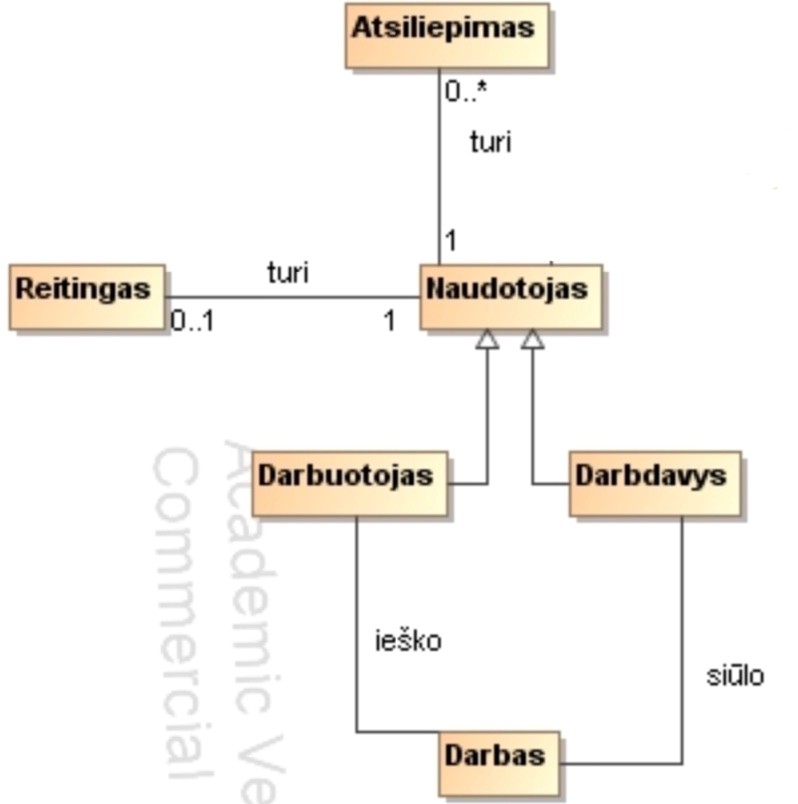
\includegraphics[scale=0.5]{img/va1.png}
\caption{Dalykinės srities struktūra}
\end{figure}

SĄVOKOS:

Šiame skyriuje pateikiami specifiniai mūsų projekte naudotų žodžių paaiškinimai.

\textbf{Sistema} – darbų valdymo sistema, dokumente vadinama „Workly“.

\textbf{Naudotojas} – asmuo, kuris naudojasi sistema. Naudotojas gali būti darbdavys, darbuotojas ir administratorius.

\textbf{Darbuotojas} – naudotojas, sistemoje ieškantis darbo.

\textbf{Darbdavys} – naudotojas, sistemoje pateikiantis darbų pasiūlymus.

\textbf{Darbas} – smulki veikla už atlygį, pasižyminti įvairiais kriterijais, kurią darbdavys patalpina sistemoje.

\textbf{Darbų sąrašas }– visų sistemoje patalpintų darbų sąrašas.

\textbf{Atsiliepimas} – komentaras, kurį gali palikti darbuotojas darbdaviui ir atvirkščiai.

\textbf{Reitingas} – skaitinis įvertinimas, kurį darbuotojas palieka darbdaviui ir atvirkščiai. Taip pat reitingu yra laikomas visų suteiktų naudotojui reitingų vidurkis.

\subsubsection{Užduotys}
\begin{figure}[H]
\centering
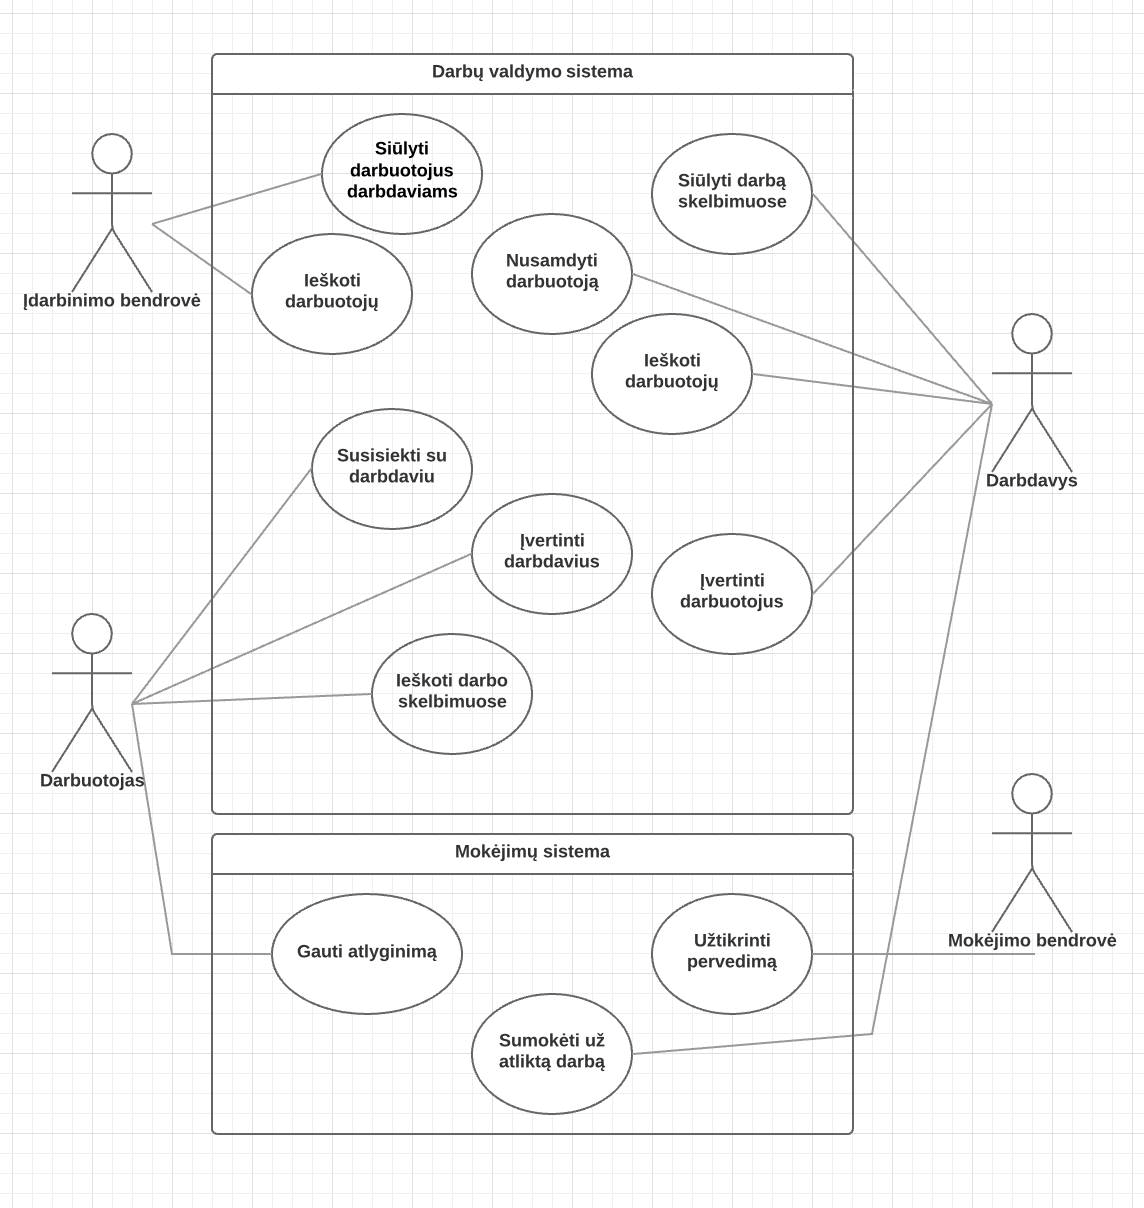
\includegraphics[width=\linewidth]{img/va2.png}
\caption{Užduočių veiklos UML diagrama}
\end{figure}

\textbf{Užduočių sąrašas (pagal 4 pav.):}

\textbf{Užduotis:} ieškoti darbuotojų.

\textbf{Tikslas:} rasti darbui tinkamą darbuotoją.

\textbf{Trigeris:} įdarbinimo bendrovės apsilankymas darbuotojų sąraše.

\textbf{Prioritetas:} aukštas.

\textbf{„Prieš” sąlygos:} egzistuoja darbuotojų.

\textbf{Sėkmingos baigties „po” sąlyga:} darbuotojas randamas ir dėl darbo susitariama.

\textbf{Nesėkmingos baigties sąlyga:} bendrovė neranda darbą atliksiančių darbuotojų.

\textbf{Pirminis agentas:} darbdavys.

\textbf{Antriniai agentai:} darbuotojas.
\\

\textbf{Užduotis:} siūlyti darbuotojus darbdaviams. 

\textbf{Tikslas:} surasti darbą darbuotojui.

\textbf{Trigeris:} darbuotojas kreipiasi su prašymu surasti jam darbą.

\textbf{Prioritetas:} vidutinis.

\textbf{„Prieš” sąlygos:} gautas prašymas iš darbuotojo.

\textbf{Sėkmingos baigties „po” sąlyga:} darbuotojui randamas darbas ir jis yra įdarbinamas.

\textbf{Nesėkmingos baigties sąlyga:} darbas nėra randamas. 

\textbf{Pirminis agentas:} įdarbinimo bendrovė.

\textbf{Antriniai agentai:} darbuotojas, darbdavys.
\\

\textbf{Užduotis:} užtikrinti pervedimą.

\textbf{Tikslas:} užtikrinti, kad atsiskaitymas už darbą pavyktų sklandžiai.

\textbf{Trigeris:} darbdavio/darbuotojo mokamas atlyginimas.

\textbf{Prioritetas:} aukštas.

\textbf{„Prieš” sąlygos:} darbdavys/darbuotojas apreiškia norą pervesti atlygį.

\textbf{Sėkmingos baigties „po” sąlyga:} atlyginimas yra pervestas sėkmingai, darbuotojas/darbdavys gauna pranešimą apie sėkmingos operacijos atlikimą.

\textbf{Nesėkmingos baigties sąlyga:} pinigų pervedimas yra nutraukiamas.

\textbf{Pirminis agentas:} mokėjimų bendrovė

\textbf{Antriniai agentai:} darbuotojas, darbdavys.
\\

\textbf{Užduotis:} įvertinti darbuotojus.

\textbf{Tikslas:} darbdavys išreiškia balais savo nuomonę apie darbuotoją.

\textbf{Trigeris}: darbuotojui atlikus darbą pas darbdavį darbdavys parenka darbuotojui balą už atiliktą darbą.
\textbf{Prioritetas:} vidutinis.

\textbf{„Prieš” sąlygos:} darbuotojas jau yra atlikęs darbą.

\textbf{Sėkmingos baigties „po” sąlyga:} darbuotojas gauna jo patikimumą labiau užtikrinantį balą.

\textbf{Nesėkmingos baigties sąlyga:} įvertinimas nepavyksta.

\textbf{Pirminis agentas:} darbdavys.

\textbf{Antriniai agentai:} darbuotojas.
\\

\textbf{Užduotis:} sumokėti už atliktą darbą.

\textbf{Tikslas:} darbdaviui atsiskaityti sutartą atlyginimą už darbuotojo darbą.

\textbf{Trigeris:} darbuotojas atliko darbą.

\textbf{Prioritetas:} aukštas.

\textbf{„Prieš” sąlygos:} susitarimas prieš darbą dėl atlygio.

\textbf{Sėkmingos baigties „po” sąlyga:} darbdavio darbas yra atliktas ir darbuotojui atsiskaitoma už jo atlikimą.

\textbf{Nesėkmingos baigties sąlyga:} darbuotojui nėra sumokamas atlygis.

\textbf{Pirminis agentas:} darbdavys.

\textbf{Antriniai agentai:} darbuotojas, mokėjimo bendrovė.
\\

\textbf{Užduotis:} ieškoti darbuotojų.

\textbf{Tikslas:} rasti darbui tinkamą darbuotoją.

\textbf{Trigeris:} darbdavio apsilankymas darbuotojų sąraše.

\textbf{Prioritetas:} aukštas.

\textbf{„Prieš” sąlygos:} egzistuoja darbuotojų.

\textbf{Sėkmingos baigties „po” sąlyga:} darbuotojas randamas ir dėl darbo susitariama.

\textbf{Nesėkmingos baigties sąlyga:} darbdavys neranda darbą atliksiančių darbuotojų.

\textbf{Pirminis agentas:} darbdavys.

\textbf{Antriniai agentai:} darbuotojas.
\\

\textbf{Užduotis}: siūlyti darbą skelbimuose.

\textbf{Tikslas:} įkelti darbo pasiūlymą į svetainę.

\textbf{Trigeris:} darbdavio darbo pasiūlymo formos užpildymas ir įkėlimas.

\textbf{Prioritetas:} aukštas.

\textbf{„Prieš” sąlygos:} naudotojas prisijungęs kaip darbdavys ir sistemoje yra darbuotojų ieškančių darbo.

\textbf{Sėkmingos baigties „po” sąlyga:} darbo pasiūlymas patalpinamas ir randamas darbuotojas.

\textbf{Nesėkmingos baigties sąlyga:} nepavyksta įkelti darbo pasiūlymo.

\textbf{Pirminis agentas:} darbdavys.

\textbf{Antriniai agentai:} darbuotojas.
\\

\textbf{Užduotis:} ieškoti darbo skelbimuose.

\textbf{Tikslas:} rasti darbą.

\textbf{Trigeris:} darbuotojo apsilankymas darbo pasiūlymų svetainėje.

\textbf{Prioritetas:} aukštas.

\textbf{„Prieš” sąlygos:} egzistuoja darbo pasiūlymų.

\textbf{Sėkmingos baigties „po” sąlyga:} darbuotojas sutaria su darbdaviu dėl darbų atlikimo.

\textbf{Nesėkmingos baigties sąlyga:} darbuotojas neranda dominančių pasiūlymų arba nesudomina darbdavių.

\textbf{Pirminis agentas:} darbuotojas.

\textbf{Antriniai agentai:} darbdavys, įdarbinimo bendrovė.
\\

\textbf{Užduotis:} susisiekti su darbdaviu.

\textbf{Tikslas:} gauti dominančio darbdavio kontaktus.

\textbf{Trigeris:} darbuotojas rado dominantį skelbimą.

\textbf{Prioritetas:} aukštas.

\textbf{„Prieš” sąlygos:} egzistuoja dominančių darbo pasiūlymų.

\textbf{Sėkmingos baigties „po” sąlyga:} darbuotojas susitaria dėl darbo sąlygų su darbdaviu.

\textbf{Nesėkmingos baigties sąlyga:} susisiekimui nepavykus darbuotojas negauna norimo darbo.

\textbf{Pirminis agentas:} darbuotojas.

\textbf{Antriniai agentai:} darbdavys.
\\

\textbf{Užduotis:} įvertinti darbdavius.

\textbf{Tikslas:} darbuotojas išreiškia balais savo nuomonę apie darbdavį.

\textbf{Trigeris:} darbuotojas atlikęs darbą pas darbdavį parenka reitingą darbdaviui.

\textbf{Prioritetas:} vidutinis.

\textbf{„Prieš” sąlygos:} darbuotojas jau yra atlikęs darbą.

\textbf{Sėkmingos baigties „po” sąlyga:} darbdavys gauna jo patikimumą labiau užtikrinantį balą.

\textbf{Nesėkmingos baigties sąlyga:} įvertinimas nepavyksta.

\textbf{Pirminis agentas:} darbuotojas.

\textbf{Antriniai agentai:} darbdavys.
\\

\textbf{Užduotis:} gauti atlyginimą

\textbf{Tikslas:} darbuotojui gauti uždirbtą atlygį iš darbdavio

\textbf{Trigeris:} darbuotojas praneša apie atliktą darbą darbdaviui.

\textbf{Prioritetas:} aukštas.

\textbf{„Prieš” sąlygos:} darbuotojas atlieka darbą.

\textbf{Sėkmingos baigties „po” sąlyga:} darbas yra gerai atliktas ir darbdavys sumoka atlyginimą.

\textbf{Nesėkmingos baigties sąlyga:} atlyginimas nėra išmokamas.

\textbf{Pirminis agentas:} darbuotojas.

\textbf{Antriniai agentai:} darbdavys, mokėjimo bendrovė.

\subsubsection{Užduočių vykdymo scenarijai}

\begin{figure}[H]
\centering
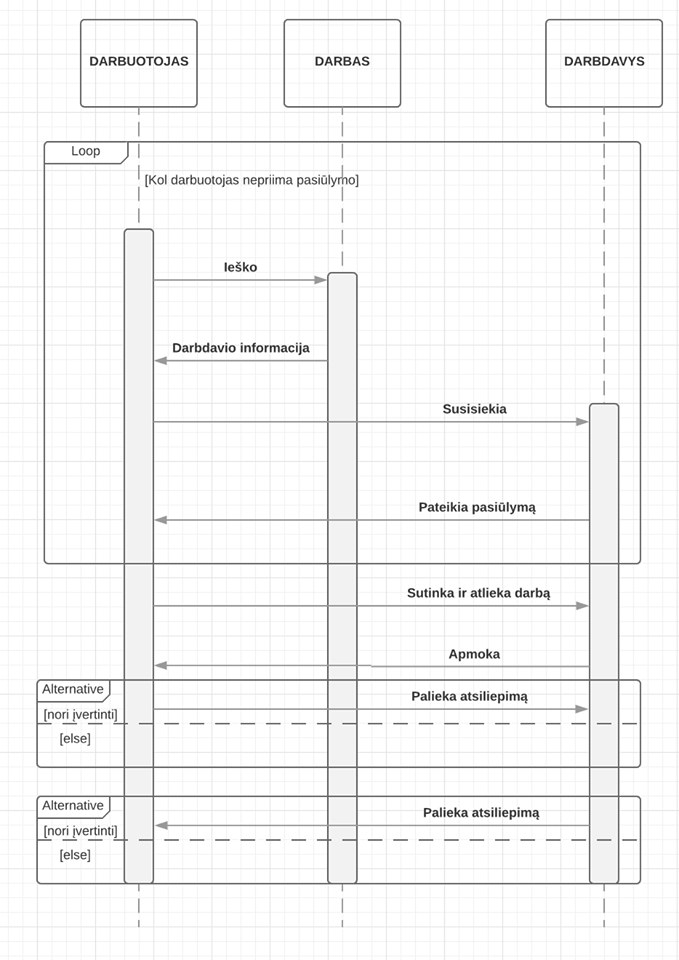
\includegraphics[scale=0.5]{img/va6.png}
\caption{Darbdavio UML būsenų diagrama}
\end{figure}
5 pav. vaizuduojamas darbo paieškos modelis. Prisijungęs darbuotojas skelbimų puslapyje gali ieškoti darbo pasiūlymų. Radęs patikusio darbo darbdavio informaciją gali su juo susisiekti. Darbdaviui išdėsčius pasiūlymą, darbuotojas gali atsisakyti ir toliau ieškoti kitų pasiūlymų arba atlikti sutartą darbą. Po darbo atlikimo abu tiek darbdavys, tiek darbuotojas turi galimybę palikti vienas kitam atitinkamą reitingą.

\subsubsection{Dalykinės srities dinaminė struktūra}

Darbdavys:
\begin{figure}[H]
\centering
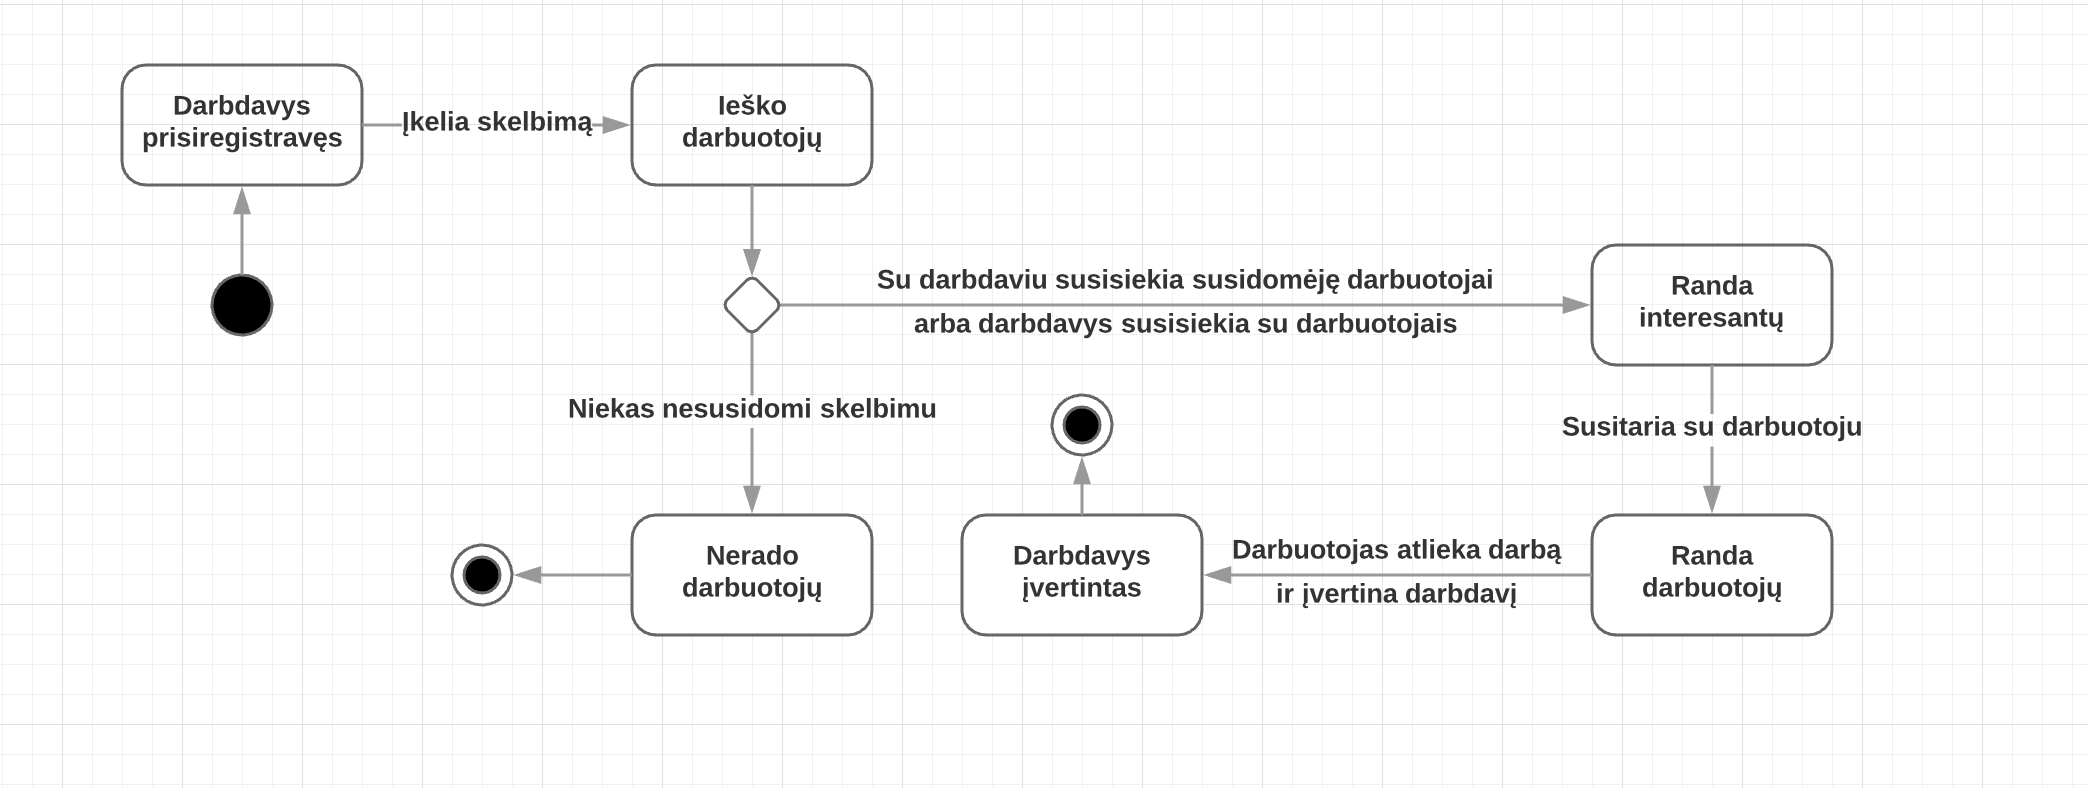
\includegraphics[width=\linewidth]{img/va3.png}
\caption{Darbdavio UML būsenų diagrama}
\end{figure}
Užsiregistravęs darbdavys turi galimybę įkelti darbo skelbimą (6 pav.). Tokiu būdu vykdoma darbuotojų paieška. Jei skelbimu kas nors susidomi arba pats darbdavys randa darbuotoją, yra susitariama dėl darbo telefonu arba el. paštu ir darbas yra atliekamas. Atlikus darbą darbdavys yra įvertinamas darbuotojo 1-5 balų skalėje. Kitas atvejis yra, kuomet niekas nesusidomi darbu ir darbuotojas darbui atlikti nėra randamas.

Skelbimas:
\begin{figure}[H]
\centering
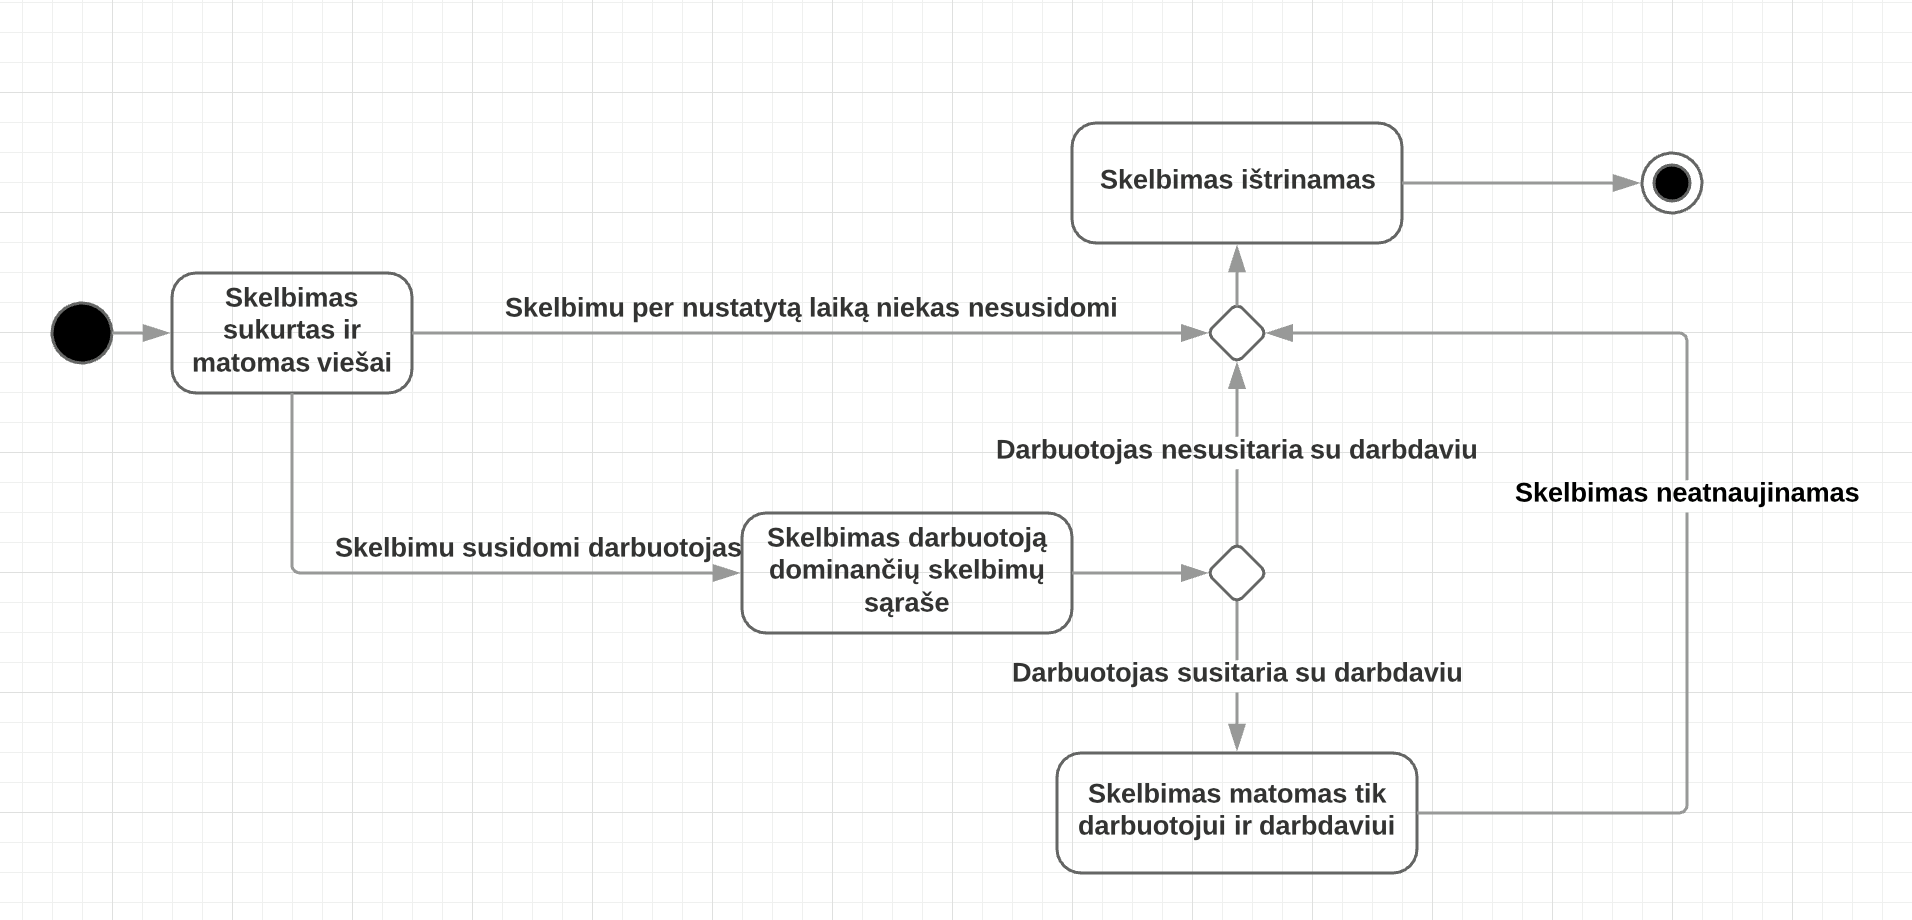
\includegraphics[width=\linewidth]{img/va4.png}
\caption{Skelbimo UML būsenų diagrama}
\end{figure}
Kuomet skelbimas sukurtas ir matomas viešai, kaip matome (7 pav.), skelbimas per tam tikrą laiko tarpą nesulaukęs susidomėjimo tampa neaktyviu ir yra šalinamas. Tačiau, jei skelbimu yra susidomima, darbuotojas gali prisidėti skelbimą į dominančių darbų sąrašą. Tuomet, darbuotojas gali sutarti su darbdaviu dėl darbo ir po darbo atlikimo skelbimas yra ištrinamas.

Darbuotojas:
\begin{figure}[H]
\centering
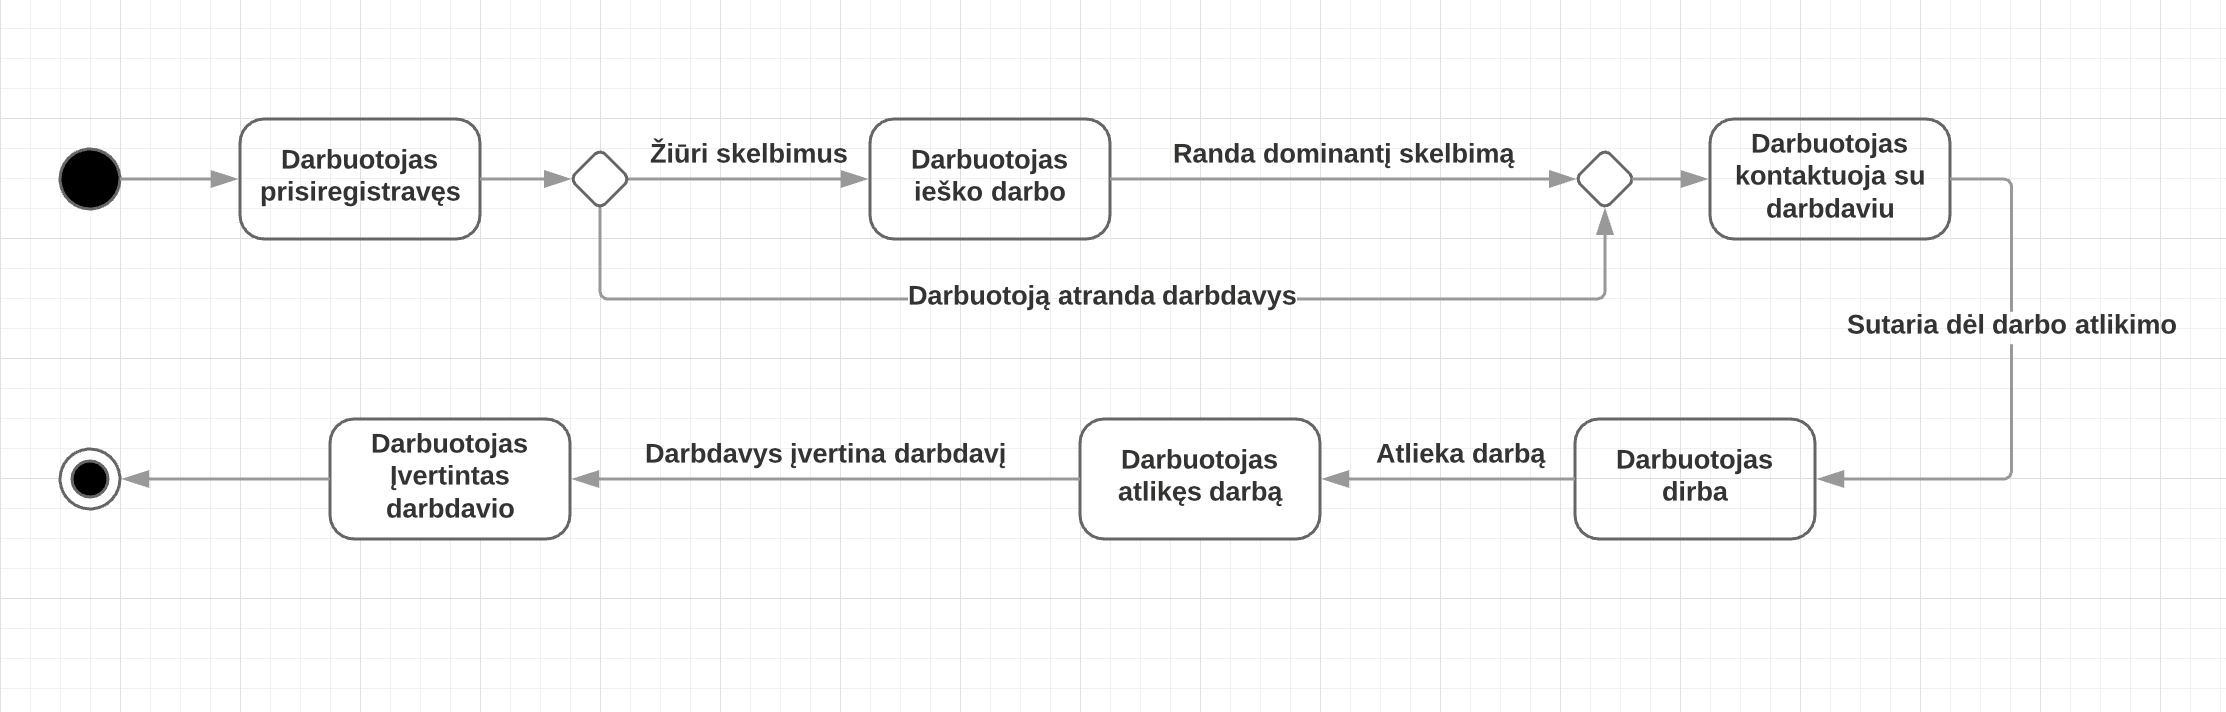
\includegraphics[width=\linewidth]{img/va5.png}
\caption{Darbuotojo UML būsenų diagrama}
\end{figure}
Užsiregistravęs darbuotojas pats ieškosi darbo žiūrėdamas skelbimus arba jį atranda darbdavys. Tuomet darbuotojas tariasi su darbdaviu dėl darbo sąlygų ir sutaria dėl atlygio. Atlikus darbuotojui darbą darbdavys įvykdo visas numatytas sąlygas ir įvertina darbuotoją reitingu nuo 1 – 5 balų.(8 pav.)
\newpage
\subsection{IŠORINĖS IR VIDINĖS ANALIZĖS REZULTATAI}
Šiame skyriuje pateikiama išorinės ir vidinės analizės pasinaudojant SSGG (SWOT) lentelės pavidalu. Lentelėje pateikiamos verslo stiprybės, silpnybės, jam kylančios grėsmės ir atsiradusios neišnaudotos galimybės (2 lentelė).
\begin{table}[H]
\caption{Analizės rezultatai SSGG lentelės pavidalu.}
\centering
\normalsize
\begin{tabular}{|p{8cm}|p{8cm}|}
\hline
\rowcolor{gray!40}

\multicolumn{1}{|m{8cm}|}{\textbf{STIPRYBĖS}}&\multicolumn{1}{m{8cm}|}{\textbf{SILPNYBĖS}}\\ \hline
\multicolumn{1}{|m{8cm}|}{
•	Centralizuota darbo pasiūlymų sistema.

•	Naudotojas turi galimybę greitai rasti trumpalaikį darbą ar žmogų padedantį atlikti darbą.

•	Patogi paieškos sistema.

•	Visi naudotojai turi reitingus, todėl užtikrinamas darbuotojų ir darbdavių patikimumas.

•	Unikalus sistemos įgyvendinimas lyginant su panašiomis sistemomis.

•	Sistema galima naudotis nemokamai.}
&\multicolumn{1}{m{8cm}|}{
•	Reitingai ir atsiliepimai yra vieninteliai užtikrinantys naudotojo patikimumą. 

•	Naujas naudotojas gali susidurti su sunkumais gaunant darbą ar ieškant darbuotojo.

•	Darbdavys prieš priimdamas darbuotoją į darbą nėra visiškai užtikrintas dėl darbuotojo.

•	Darbuotojas prieš pradedant dirbti nėra visiškai užtikrintas dėl darbdavio.

•	Reklamos trūkumas.

•	Sistema neturi galimybės atlikti atsiskaitymų už darbą, todėl mokėjimai yra vykdomi bendru darbdavio ir darbuotojo susitarimu.
}\\ \hline
\rowcolor{gray!40}
\multicolumn{1}{|m{8cm}|}{\textbf{GALIMYBĖS}}&\multicolumn{1}{m{8cm}|}{\textbf{GRĖSMĖS}}\\ \hline
\multicolumn{1}{|m{8cm}|}{
•	Tapti patogiausia tokio tipo programa naudotojui  Lietuvoje.

•	VIP darbo pasiūlymų galimybė

•	Vystyti reklamą socialiniuose tinkluose, televizijoje ir kitose viešosiose erdvėse.

•	Mobili aplikacija.

•	Suteikti atsiskaitymo galimybes. 

•	Skambintii darbuotojui/darbdaviui vieno mygtuko paspaudimu.

•	Darbo pasiūlymų rūšiavimas pagal dabartinę vietą.

}&\multicolumn{1}{m{8cm}|}{
•	Naujos sistemos nežinomumas. Galimas naudotojų stygius.

•	Reklamos neefektyvumas.

•	Didelė konkurencija šioje srityje.

•	Galimi nauji konkurentai su pranašesnėmis sistemomis

•	Žmonių nesąžiningumas (netikrų anketų kūrimas, netikrų darbo pasiūlymų kūrimas) sumažins naudotojų skaičių ir pakenks sistemos patikimumui.

}\\ \hline

\end{tabular}
\end{table}

\newpage
\subsection{VERSLO PROCESO TOBULINIMO STRATEGIJA}
Šiame skyriuje aprašomas pagrindinis kuriamo verslo proceso tikslas bei kokios strategijos bus naudojamos norint įgyvendinti tikslą.

\subsubsection{Vizija}
\textbf{Vizija}  - greita ir patogi greitų (laikinų) darbo pasiūlymų paieška bei pateikimas.

\subsubsection{Misija}
\textbf{Misija}  - sukurti darbo pasiūlymų valdymo sistema, kuri pateiktų greitus (laikinus) darbo pasiūlymus vienoje vietoje, suteiktų galimybę greitai susirasti norimą darbo pasiūlymą, susirasti sau tinkamą darbuotoją ar darbdavį.

\subsubsection{Strateginiai ir operaciniai tikslai}
Pagrindinis ir ilgalaikis kuriamo verslo proceso tikslas - palengvinti darbų paiešką, užtikrinti objektyvų darbuotojų ir darbdavių vertinimą. Šiame skyriuje pateikiami pagrindiniai kuriamo verslo proceso stateginiai tikslai ir opearaciniai tikslai.\\ \\
\hspace*{1cm}1. Sukurti patogesnį darbų valdymo sistemos naudojimąsi.\\
\hspace*{2cm} a) Sukurti internetinę svetainę.\\
\hspace*{2cm} b) Patobulinti grafinę vartotojo sąsają, kad 80\% naudotojų ją vertintų teigiamai.\\ \newline
\hspace*{1cm}2. Sukurti patogią darbų įkėlimo ir paieškos sistemą.\\
\hspace*{2cm} a) Galimybė redaguoti įkeltus darbo pasiūlymus.\\
\hspace*{2cm} b) Galimybė ieškoti darbo pagal raktinį žodį.\\
\hspace*{2cm} c) Galimybė rikiuoti duomenis pagal vietovę, trukmę, darbo sritį, užmokestį.\\
\hspace*{2cm} d) Galimybė darbdaviams matyti įkeltus darbo pasiūlymus.\\
\hspace*{2cm} e) Galimybė darbuotojams matyti jau peržiūrėtus ir dominančius darbo pasiūlymus.\\
\hspace*{2cm} f) Galimybė įkelti VIP darbo pasiūlymus.\\
\hspace*{1cm}3. Sukurti darbuotojų ir darbdavių vertinimo sistemą.\\
\hspace*{2cm} a) Galimybė reitinguoti darbuotojus ir darbdavius.\\
\hspace*{2cm} b) Galimybė rašyti atsiliepimus apie darbuotojus ir darbdavius.\\
\hspace*{2cm} c) Galimybė pamatyti darbdavio reitingą iš rekvizitai.lt.\\
\hspace*{1cm}4. Didinti sistemos žinomumą.\\
\hspace*{2cm} a) Sukurti Facebook puslapį.\\
\hspace*{2cm} b) Įkelti bent 2 reklamas per mėnesį į socialinius tinklus.\\ \newline
\hspace*{1cm}5. Skatinti naudotojų aktyvumą.\\
\hspace*{2cm} a) Aktyviausiams naudotojams dovanoti prizus (pvz.: nemokamas VIP darbo pasiūlymas).\\ \newline
\hspace*{1cm}6. Pridėti papildomo sistemos funkcionalumo.\\
\hspace*{2cm} a) Sukurti patogią apmokėjimo sistemą.\\
\hspace*{2cm} b) Įgalinti automatinį skambinimą darbdaviui/darbuotojui vienu mygtuko paspaudimu.\\
\hspace*{2cm} c) Pateikiamas darbo pasiūlymų sąrašas, kurių atlikimo vieta ir netoli darbartinės naudotojo vietos.\\

\newpage
\subsection{SISTEMOS NAUDOJIMO SCENARIJUS}
Šiame skyriuje aprašomas darbų valdymo sistemos naudojimo scenarijus.
\subsubsection{Scenarijus}
Šiame skyriuje pateikiami pagrindinių funkcijų modeliai, kurie parodo, kaip pagrindiniai sistemos agentai, šiuo atveju darbuotojai ir darbdaviai, naudosis sistema. Tam naudojamos UML sekų diagramos.
\subsubsubsection{Užduoties registruotis modelis}
\begin{figure}[H]
\centering
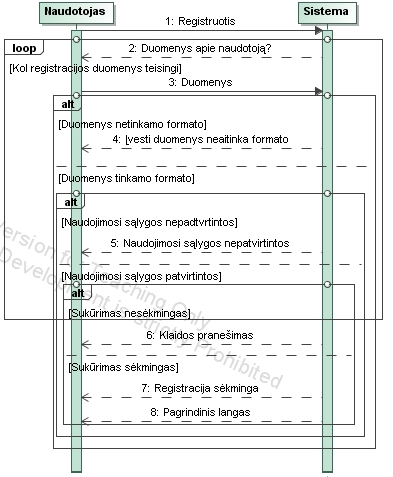
\includegraphics[scale=1]{img/registracija.png}
\caption{Įeigos, išeigos, įvaizdžio ir reguliavimo analizės diagrama}
\end{figure}
\textbf{Užduotis:} užregistruoti naują naudotoją (9 pav.).

\textbf{Verslo sistema:} darbo pasiūlymų valdymo sistema.

\textbf{Tikslas:} pradėti naudotis darbo pasiūlymų sistema.

\textbf{Pirminis agentas:} naudotojas.

\textbf{„Prieš“ sąlyga:} naudotojas atsidaręs sistemos tinklalapį.

\textbf{„Po“ sąlyga:} naudotojas gali pridėti arba ieškoti darbų.

\textbf{Scenarijus:} naudotojas, atsidaręs sistemos internetinį puslapį ir užėjęs į registracijos formą, turi įvesti savo duomenis: vardą, pavardę, telefono numerį, el. pašto adresą, slaptažodį du kartus ir pasirinkti, ar nori užsiregistruoti kaip darbuotojas ar kaip darbdavys. Naudotojas registracijos formoje taip pat turi pažymėti, kad sutinka su sistemos sąlygomis. Jeigu įvesti duomenys neatitinka formato arba toks klientas jau yra registruotas, naudotojui parodomas klaidos pranešimas. Jeigu registracija sėkminga, naudotojui yra pranešama apie sėkmingą registraciją ir jis yra nukreipiamas į pagrindinį sistemos puslapį.

\subsubsubsection{Užduoties sukurti darbo pasiūlymą modelis}
\begin{figure}[H]
\centering
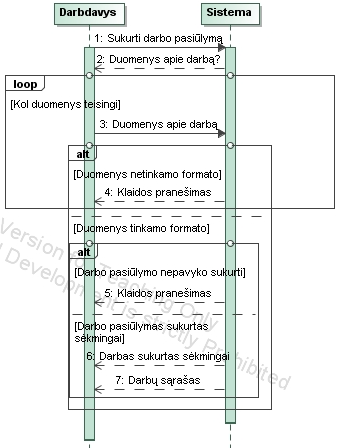
\includegraphics[scale=1]{img/sukurtiDarba.png}
\caption{Užduoties sukurti darbo pasiūlymą modelis}
\end{figure}

\textbf{Užduotis:} sukurti darbo pasiūlymą (10 pav.).

\textbf{Verslo sistema:} darbo pasiūlymų valdymo sistema.

\textbf{Tikslas:} sukurti darbo pasiūlymą sistemoje.

\textbf{Pirminis agentas:} darbdavys.

\textbf{„Prieš“ sąlyga:} darbdavys yra prisijungęs prie sistemos.

\textbf{„Po“ sąlyga:} darbdavys sėkmingai sukūrė darbo pasiūlymą.

\textbf{Scenarijus:} norėdamas sukurti darbo pasiūlymą, darbdavys pasirenka darbo sukūrimo puslapį ir gražintoje formoje suveda darbo informacija: vietą, atlygį, numatomą trukmę, darbo pavadinimą ir kokiai sričiai priklauso darbo pasiūlymas. Jeigu duomenys neatitinka formato, sistema įspėja darbdavį ir leidžia pakeisti duomenis. Jeigu duomenys atitinka formatą, darbdavys yra informuojamas apie sėkmingą pasiūlymo išsaugojimą sistemoje.

\subsubsubsection{Užduoties ieškoti darbo pasiūlymo modelis}
\begin{figure}[H]
\centering
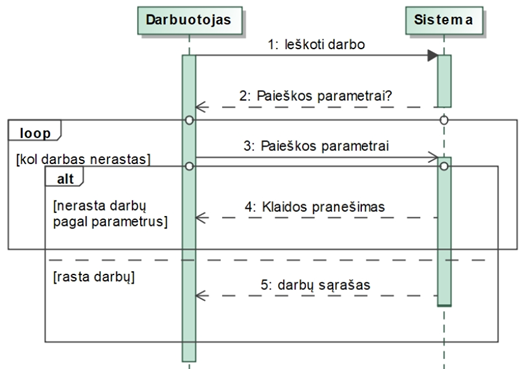
\includegraphics[scale=1]{img/ieskoti.png}
\caption{Užduoties ieškoti darbo pasiūlymo modelis}
\end{figure}

\textbf{Užduotis:} rasti darbo pasiūlymą. (11 pav.).

\textbf{Verslo sistema:} darbo pasiūlymų valdymo sistema.

\textbf{Tikslas:} rasti darbo pasiūlymą sistemoje.

\textbf{Pirminis agentas:} darbuotojas.

\textbf{„Prieš“ sąlyga:}  darbuotojas yra prisijungęs prie sistemos.

\textbf{„Po“ sąlyga:} darbuotojas sėkmingai rado darbo pasiūlymą.

\textbf{Scenarijus:} norėdamas surasti darbo pasiūlymą, darbuotojas įveda ieškomo darbo parametrus. Tai gali būti atlygis, darbo vieta, trukmė, darbo pavadinimas ar darbo sritis. Jeigu sistema nesuranda paieškos parametrus tenkinančio darbo, darbuotojas gali juos pakeisti. Sistemai suradus darbą, darbuotojui yra pateikiamas paieškos parametrus atitinkančių darbo pasiūlymų sąrašas. 

\subsubsection{Sistemos teikiama nauda}
Šiame skyriuje nagrinėjamos užduotys, kurias gali atlikti naudotojai. Tam pavaizduoti naudojama UML užduočių diagrama, kurioje agentai yra mūsų sistemos naudotojai - darbuotojai ir darbdaviai.
\begin{figure}[H]
\centering
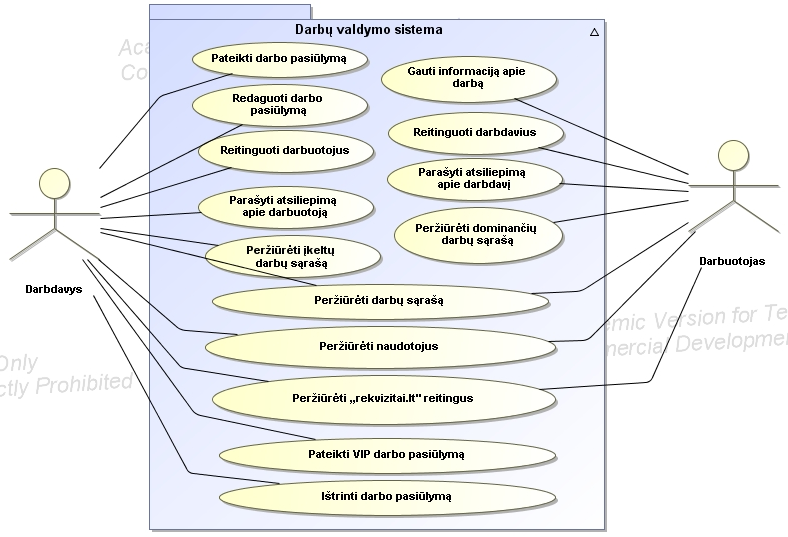
\includegraphics[scale=0.7]{img/usecase2.png}
\caption{Užduočių diagrama}
\end{figure}
Sistemoje vykdomos pagrindinės užduotys: darbuotojas gali susirasti ieškomą darbą, reitinguoti darbdavius, peržiūtėti dominančius darbo pasiūlymus. Darbdavys siekia pateikti, redaguoti ar ištrinti darbo pasiūlymą, reitinguoti darbuotojus, peržiūrėti įkeltus darbus  ar įkelti VIP darbo pasiūlymą. Ir darbdavys, ir darbuotojas nori peržiūrėti darbų sąrašą, peržiūrėti TOP darbdavius ir darbuotojus, parašyti atsiliepimus (12 pav.).
\subsubsection{Esama būklė}
Šiuo metu visi komandos nariai turi asmeninius kompiuterius kuriais gali kurti ir testuoti sistemą. Nariai taip pat turi priėjimą prie Android ir iOS išmaniųjų telefonų, kurių prireiks tinklapio testavimui mobiliuose įrenginiuose. Grupė sudaryta iš keturių asmenų, kurie yra įgiję reikalingas žinias sistemos sukūrimui ir palaikymui. 
\subsubsection{Priemonės scenarijui įgyvendinti.}
Norint sukurti darbų valdymo sistemą bus reikalinga:\\
\hspace*{2cm} 1. Domeno registracija\\
\hspace*{2cm} 2. Serveris\\
\hspace*{2cm} 3. SSL sertifikatas\\

\newpage
\subsection{ĮGYVENDINAMUMO IR NAUDOS ANALIZĖ}
Šiame skyriuje pateikiama informacija, kuri padeda nustatyti, ar darbų valdymo sistemą įmanoma sukurti, kokią konkrečią naudą ji duos, kokios problemos gali kilti ir kaip jos bus sprendžiamos.
\subsubsection{Operacinis įgyvendinamumas}
Šiame skyriuje pateikiami galimi trukdžiai, kurie gali kilti naudantis sistema, bei pateikiami galimi jų sprendimo būdai.\\ \newline
\textbf{Problema: }darbuotojai gali nepasitikėti darbdaviais, kurių įvertinimas yra žemas arba dar neturi nė vieno atsiliepimo.\\
\textbf{Problemos sprendimas: } įdiegti ESCROW atsiskaitymo sistemą užtikrinti darbdavio mokumui.\\  \newline
\textbf{Problema: }labai mažas darbdavių skaičius gali pirkti mokamus VIP darbo pasiūlymus.\\
\textbf{Problemos sprendimas: } konsultuotis su reklamos specialistais, kurie pagelbėtų įtikinti darbdavius investuoti į VIP skelbimus. \\  \newline
\textbf{Problema: }darbuotojai gali nesinaudoti sistema dėl darbų trūkumo.\\
\textbf{Problemos sprendimas: }įdiegti asmeninių pakvietimų sistemą, kuri skatintų esamus darbdavius kviesti naujus klientus užsiregistruoti sistemoje. Už pakviestus ir prisiregistravusius aktyvius darbdavius, pakvietimo kodo siuntėjas gautu nemokamų VIP skelbimų. \\  \newline
\textbf{Problema: }darbdaviai gali nesinaudoti sistema dėl darbuotųjų trūkumo.\\
\textbf{Problemos sprendimas: }konsultuotis su reklamos specialistais, kurie padėtų efektyviau pasiekti neterminuoto darbo ieškančius žmones ir skatinti naudotis sistema. \\ \newline
\textbf{Problema: }naudotojai gali naršyti reklamą blokuojančiomis interneto naršyklėmis.\\
\textbf{Problemos sprendimas: }aptikus reklamos blokavimą, iškelti pranešimą rekomenduojantį išjungti filtrą. \\  \newline
\textbf{Problema: }klientams sistema gali pasirodyti sudėtinga naudotis.\\
\textbf{Problemos sprendimas: }Užsiregistravus sistemoje naujam naudotojui, jis bus nukreiptas į įžangą apie naudojimąsi darbų valdymo sistema „Workly".\\ 

\subsubsection{Techninis įgyvendinamumas}
Rinkoje egzistuoja daug panašių darbų valdymo sistemų, todėl kuriama sistema nereikalauja sunkiai įgyvendinamų sprendimų. Sistema bus prieinama tik internetu, todėl vartotojai privalės turėti priėjimą prie interneto. Dauguma darbingo amžiaus žmonių turi išmaniuosius telefonus arba kompiuterius namuose, kuriais gali pasiekti interneto paslaugas, taigi sistema yra techniškai įgyvendinama. Sistemos kūrimo komanda neturi daug patirties kuriant internetinius puslapius, tačiau yra sudaryta iš programų sistemų bakalauro kurso studentų. Grupė yra susipažinusi su internetiniams puslapiams aktualiomis sritimis kaip objektinis programavimas, API programavimas, duomenų bazių projektavimas. Taip pat, dalis komandos narių yra savarankiškai dirbę su MVC šablonu ir turi front-end programavimo žinių. Šių techninių įgūdžių pakanka įgyvendinti sistemai.

\subsubsection{Ekonominis įgyvendinamumas}
\textbf{Išlaidos}

Numatoma sistemos sukūrimo kaina – 5120 €. Ši suma apskaičiuota numatant, kad sistemos kūrimo procesas užtruks 14 savaičių dirbant keturiems žmonėms po pusę etato. Alga 4 €/h.

Sistemos palaikymo kaina – 320€ / mėn. Tai yra prognozuojama vieno darbuotojo, dirbančio pusę etato, apmokamo 4 €/h alga.

Kitas išlaidos pateikiamos 2 lentelėje.
\begin{table}[H]
\caption{Išlaidos reikalingos sistemos sukūrimui ir palaikymui}
\centering
\normalsize
\begin{tabular}{|p{8cm}|p{4cm}|}
\hline
\rowcolor{gray!40}
\multicolumn{1}{|m{8cm}|}{\textbf{IŠLAIDOS}}&\multicolumn{1}{m{4cm}|}{\textbf{KAINA}}\\ \hline
\multicolumn{1}{|m{8cm}|}{Domeno registracija}&\multicolumn{1}{m{4cm}|}{8€}\\ \hline
\multicolumn{1}{|m{8cm}|}{Programos sukūrimas}&\multicolumn{1}{m{4cm}|}{5120€}\\ \hline
\multicolumn{1}{|m{8cm}|}{Serverio nuoma svetainei}&\multicolumn{1}{m{4cm}|}{48 € metams}\\ \hline
\multicolumn{1}{|m{8cm}|}{Domeno registracijos pratęsimasi}&\multicolumn{1}{m{4cm}|}{10€}\\ \hline
\multicolumn{1}{|m{8cm}|}{SSL sertifikatas}&\multicolumn{1}{m{4cm}|}{44€ metams}\\ \hline
\multicolumn{1}{|m{8cm}|}{Sistemos palaikymas sukūrus}&\multicolumn{1}{m{4cm}|}{320€ / mėn}\\ \hline
\multicolumn{1}{|m{8cm}|}{Reklama}&\multicolumn{1}{m{4cm}|}{50€ / mėn}\\ \hline
\end{tabular}
\end{table}
\textbf{Iš viso:}

Sistemos sukūrimo kaštai: 5128€

Kaštai per metus: 4542€\\ 

\textbf{Pajamos}

Pagridinis kuriamos sistemos pajamų šaltinis VIP darbo pasiūlymai. Atsižvelgiant į rinkos kainą, vienas VIP darbo pasiūlymas kainuotų 0.75€ vienai dienai. Darome prielaidą, kad per mėnesį vidutiniškai bus sudaroma apie 400 VIP darbo pasiūlymų. Todėl kuriamos sistemos pajamos  - 4500€ per metus.

Taip pat programėlė planuoja gauti pajamas talpindama reklamą savo svetainė (Google adsense) 200€ per mėnesį.
\begin{table}[H]
\caption{Pajamos iš kuriamo verslo proceso}
\centering
\normalsize
\begin{tabular}{|p{8cm}|p{4cm}|}
\hline
\rowcolor{gray!40}
\multicolumn{1}{|m{8cm}|}{\textbf{IŠLAIDOS}}&\multicolumn{1}{m{4cm}|}{\textbf{KAINA}}\\ \hline
\multicolumn{1}{|m{8cm}|}{VIP darbo pasiūlymai}&\multicolumn{1}{m{4cm}|}{375€/mėn}\\ \hline
\multicolumn{1}{|m{8cm}|}{Reklama}&\multicolumn{1}{m{4cm}|}{200€/mėn}\\ \hline
\end{tabular}
\end{table}
Iš viso pajamų: 6900€ per metus  (4 lentelė)\\

\textbf{Pelnas/Nuostolis}\\
Darbų valdymo sistema per metus uždirbtų 2358€  (atmetus kasmetinius kaštus). Sistemos sukūrimo kaštus sistema padengtų maždaug per dvejus metus (1,9 metų). Taigi, pirmus dvejus metus sistema neduotų pelno, tačiau po dviejų metų būtų galima tikėtis 2358€ pelno per metus.
\subsubsection{Juridinis įgyvendinamumas}
Įmonės veikla nepažeis asmenų duomenų apsaugos įstatymų, Europos sąjungos direktyvų ir Lietuvos respublikos konstitucijos. Kliento duomenys yra tvarkomi tiksliai ir perduodami užšifruota sąsaja. Įmonės darbuotojams mokamas didesnis negu minimalus atlyginimas ir darbas vyksta laisvu grafiku. Sistemos klientai yra patys atsakingi už atitinkamų įstatymų laikymąsi ir mokesčių mokėjimą.
\newpage
\section{REIKALAVIMŲ SPECIFIKAVIMAS}
Dokumente pateikiamos savybės, kuriomis turi pasižymėti sistema, kreipiamas dėmesys į ribotus jos kūrimo išteklius. Reikalavimai sunumeruoti - tai padeda juos lengviau identifikuoti.
%FUNKCINIAI REIKALAVIMAI
\subsection{FUNKCINIAI REIKALAVIMAI}
1 skyriuje pateikiami funkciniai reikalavimai – aprašoma, ką sistema turi daryti. Analizuojamos iš sistemos naudotojo reikalaujamos užduotys, nagrinėjami scenarijai, kaip sistema turėtų elgtis vienu ar kitu atveju. Apibrėžiant funkcinius reikalavimus naudojamos procesų sekų diagramos, sistemoje vykdomų užduočių diagrama (žr. 1.6.2).

%%%%%%%%%%%%%%%%%%%%%%%%%%%%%%
\subsubsection{Internetinės svetainės langai}
\begin{table}[H]
\caption{Funkciniai reikalavimai. Internetinės svetainės langai}
\centering
\normalsize
\begin{tabular}{|p{2cm}|p{10cm}|p{3cm}|}
\hline
\rowcolor{gray!30}
\multicolumn{3}{|l|}{\textbf{1. Internetinės svetainės langai}} \\ \hline
\textbf{KODAS}& \multicolumn{1}{m{10cm}|}{\textbf{REIKALAVIMAS}} & \textbf{SVARBA} \\ \hline
FR1.1 & \multicolumn{1}{m{10cm}|}{Svetainės langai Titulinis puslapis,  ,,Kontaktai“, „Registracija“, „Prisijungimas“ matomi visiems net ir neprisijungusiems naudotojams.} & Būtinas \\ \hline
FR1.2 & \multicolumn{1}{m{10cm}|}{Svetainės langai „Darbai“, „Naudotojai“ yra matomi prisijungusiems naudotojams.} & Būtinas \\ \hline
FR1.3 & \multicolumn{1}{m{10cm}|}{Svetainės langas „Dominantys darbo pasiūlymai“ matomas tik darbuotojams.} & Būtinas \\ \hline
FR1.4 & \multicolumn{1}{m{10cm}|}{Svetainės langas „Įkelti darbo pasiūlymai“ matomas tik darbdaviams.} & Būtinas \\ \hline
\end{tabular}
\end{table}

%%%%%%%%%%%%%%%%%%%%%%%%%%%%%%%
\subsubsection{Prisijungimas}
\begin{table}[H]
\caption{Funkciniai reikalavimai. Prisijungimas}
\centering
\normalsize
\begin{tabular}{|p{2cm}|p{10cm}|p{3cm}|}
\hline
\rowcolor{gray!30}
\multicolumn{3}{|l|}{\textbf{2. Prisijungimas}} \\ \hline
\textbf{KODAS}& \multicolumn{1}{m{10cm}|}{\textbf{REIKALAVIMAS}} & \textbf{SVARBA} \\ \hline
FR2.1 & \multicolumn{1}{m{10cm}|}{Naudotojui suvedus tinkamą el. pašto adresą ir slaptažodį jis yra prijungiamas prie sistemos.} & Būtinas \\ \hline
FR2.2 & \multicolumn{1}{m{10cm}|}{Naudotojui neįvedus (įvedus netinkamo formato) el. pašto arba slaptažodžio laukus, laukai yra nuspalvinami raudonai ir išvedamas klaidos tekstas.} & Būtinas \\ \hline

\end{tabular}

\end{table}

\begin{table}[H]
\centering
\normalsize
\begin{tabular}{|p{2cm}|p{10cm}|p{3cm}|}
\hline
FR2.3 & \multicolumn{1}{m{10cm}|}{Naudotojui įvedus netinkamus prisijungimo duomenis išvedamas pranešimas, kad prisijungimas nesėkmingas.} & Būtinas \\ \hline
FR2.4 & \multicolumn{1}{m{10cm}|}{Turi būti galimybė užmiršus slaptažodį gautį jį į registracijos metu nurodytą el.paštą.} & Būtinas \\ \hline
FR2.5 & \multicolumn{1}{m{10cm}|}{Turi būti galimybė išsaugoti prisijungimo metu įvestus duomenis (kad kitą kartą prisijungus nereikėtų įvesti iš naujo).} & Būtinas \\ \hline
FR2.6 & \multicolumn{1}{m{10cm}|}{Naudotojų bandymų prisijungti prie sistemos skaičius nėra ribojamas.} & Būtinas \\ \hline
\end{tabular}

\end{table}

13 pav. pateikiama užduoties „Prisijungimas" sekų diagrama. Joje vaizduojamas pagrindinis prisijungimo prie sistemos scenarijus ir taip pat nagrinėjami alternatyvūs scenarijai.
\begin{figure}[H]
\centering
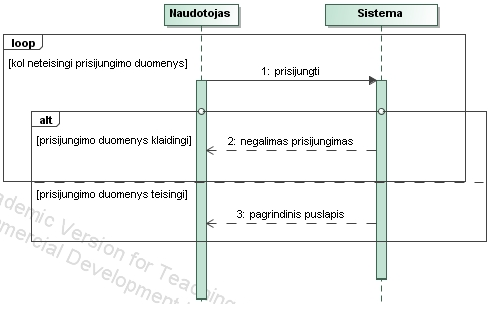
\includegraphics[scale=1, frame]{img/prisijungimas.png}
\caption{Proceso „Prisijungimas" sekų diagrama}
\end{figure}
%%%%%%%%%%%%%%%%%%%%%%%%%%%%%%%%%%%

\subsubsection{Atsijungimas}
\begin{table}[H]
\caption{Funkciniai reikalavimai. Atsijungimas}
\centering
\normalsize
\begin{tabular}{|p{2cm}|p{10cm}|p{3cm}|}
\hline
\rowcolor{gray!30}
\multicolumn{3}{|l|}{\textbf{3. Atsijungimas}} \\ \hline
\textbf{KODAS}& \multicolumn{1}{m{10cm}|}{\textbf{REIKALAVIMAS}} & \textbf{SVARBA} \\ \hline
FR3.1 & \multicolumn{1}{m{10cm}|}{Naudotojas paspaudęs mygtuką atsijungti yra atjungiamas nuo sistemos.} & Būtinas \\ \hline
FR3.2 & \multicolumn{1}{m{10cm}|}{Atsijungus nuo sistemos ir bandant paspausti grįžimo mygtuką jis yra nukreipiams į prisijungimo langą.} & Būtinas \\ \hline
FR3.3 & \multicolumn{1}{m{10cm}|}{Įvykus nesėkmingam atsijungimui nuo sistemos, naudotojui išmetamas pranešimas, kad atsijungimas nepavyko ir pasiūloma pabandyti dar kartą.} & Būtinas \\ \hline
\end{tabular}
\end{table}
14 pav. pateikiama užduoties „Atsijungimas nuo sistemos" sekų diagrama. Joje vaizduojamas pagrindinis atsijungimo nuo sistemos scenarijus ir taip pat nagrinėjami alternatyvūs scenarijai.
\begin{figure}[H]
\centering
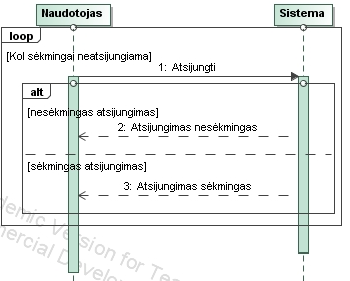
\includegraphics[scale=1, frame]{img/atsijungimas.png}
\caption{Proceso „Atsijungimas" sekų diagrama}
\end{figure}
%%%%%%%%%%%%%%%%%%%%%%%%%%%%%%%%%%%%%%
\subsubsection{Registracija}
\begin{table}[H]
\caption{Funkciniai reikalavimai. Registracija}
\centering
\normalsize
\begin{tabular}{|p{2cm}|p{10cm}|p{3cm}|}
\hline
\rowcolor{gray!30}
\multicolumn{3}{|l|}{\textbf{4. Registracija}} \\ \hline
\textbf{KODAS}& \multicolumn{1}{m{10cm}|}{\textbf{REIKALAVIMAS}} & \textbf{SVARBA} \\ \hline
FR4.1 & \multicolumn{1}{m{10cm}|}{Naudotojui įvedus savo el. pašto adresą (simbolių seka, kuri baigias @ ir domenu) – laukas validuojamas.} & Būtinas \\ \hline
FR4.2 & \multicolumn{1}{m{10cm}|}{Jei naudotojo įvestas el. paštas jau egzistuoja, išvedamas pranešimas, kad toks el. paštas jau egzistuoja.} & Būtinas \\ \hline
FR4.3 & \multicolumn{1}{m{10cm}|}{Naudotojui įvedus slaptažodį (minimaliai 6 simboliai) – laukas validuojamas.} & Būtinas \\ \hline
FR4.4 & \multicolumn{1}{m{10cm}|}{Naudotojui įvedus tinkamą (tokį pat, kaip ankstesniame lauke) pakartotą slaptažodį – laukas validuojamas.} & Būtinas \\ \hline
FR4.5 & \multicolumn{1}{m{10cm}|}{Naudotojui įvedus savo vardą (maksimalus ilgis 80 simbolių) – laukas validuojamas.} & Būtinas \\ \hline
FR4.6 & \multicolumn{1}{m{10cm}|}{Naudotojui įvedus savo pavardę (maksimalus ilgis 80 simbolių) – laukas validuojamas.} & Būtinas \\ \hline
FR4.7 & \multicolumn{1}{m{10cm}|}{Naudotojui įvedus savo telefono numerį (prasideda +370 ir dar 8 skaitmenys ) – laukas validuojamas.} & Būtinas \\ \hline
FR4.8 & \multicolumn{1}{m{10cm}|}{Naudotojui pasirinkus statusą (darbuotojas, darbdavys) – laukas validuojamas.} & Būtinas \\ \hline
\end{tabular}
\end{table}

\begin{table}[H]
\centering
\normalsize
\begin{tabular}{|p{2cm}|p{10cm}|p{3cm}|}
\hline

FR4.9 & \multicolumn{1}{m{10cm}|}{Naudotojas  prisijungimo metu turi sutikti su svetainės naudojimosi sąlygomis. Norėdamas pamatyti sąlygas naudotojas paspaudžia ant nuorodos.} & Būtinas \\ \hline
FR4.10 & \multicolumn{1}{m{10cm}|}{Naudotojui nesutikus su svetainės sąlygomis išvedamas pranešimas, kad norint prisiregistruoti reikia sutikti su svetainės naudojimosi sąlygomis.} & Būtinas \\ \hline
FR4.11 & \multicolumn{1}{m{10cm}|}{Naudotojui  suvedus tinkamus duomenis sukuriamas naujas naudotojas.} & Būtinas \\ \hline
FR4.12 & \multicolumn{1}{m{10cm}|}{Naudotojui neužpildžius privalomų laukų arba juos užpildžius netinkamai laukai yra nuspalvinami raudonai ir išvedamas klaidos tekstas.} & Būtinas \\ \hline
FR4.13 & \multicolumn{1}{m{10cm}|}{Nepavykus sukurti naujo naudotojo, naudotojas informuojamas apie sistemos klaidą ir prašoma pakartoti registraciją.} & Būtinas \\ \hline
\end{tabular}
\end{table}
15 pav. pateikiama užduoties „Registracija" sekų diagrama. Joje vaizduojamas pagrindinis registravimosi prie sistemos scenarijus ir taip pat nagrinėjami alternatyvūs scenarijai.
\begin{figure}[H]
\centering
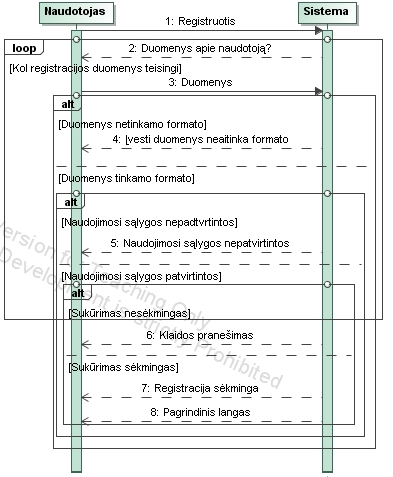
\includegraphics[scale=1, frame]{img/registracija.png}
\caption{Proceso „Registracija" sekų diagrama}
\end{figure}
%%%%%%%%%%%%%%%%%%%%%%%%%%%%%%%%%%%%
\subsubsection{Paskyros valdymas}
\begin{table}[H]
\caption{Funkciniai reikalavimai. Paskyros valdymas}
\centering
\normalsize
\begin{tabular}{|p{2cm}|p{10cm}|p{3cm}|}
\hline
\rowcolor{gray!30}
\multicolumn{3}{|l|}{\textbf{5. Paskyros valdymas}} \\ \hline
\textbf{KODAS}& \multicolumn{1}{m{10cm}|}{\textbf{REIKALAVIMAS}} & \textbf{SVARBA} \\ \hline
FR5.1 & \multicolumn{1}{m{10cm}|}{Naudotojui paspaudus ant el. pašto adreso matoma registracijos metu įvesta informacija.} & Būtinas \\ \hline
FR5.2 & \multicolumn{1}{m{10cm}|}{Naudotojui paspaudus ant mygtuko „pakeisti slaptažodį“, įvedus tinkamą seną slaptažodį, naują slaptažodį įvedus ir patvirtinus slaptažodis yra pakeičiamas į naują.} & Būtinas \\ \hline
FR5.3 & \multicolumn{1}{m{10cm}|}{Naudotojui paspaudus ant mygtuko „pakeisti slaptažodį“ ir įvedus netinkamą seną slaptažodį išvedamas klaidos pranešimas.} & Būtinas \\ \hline
FR5.4 & \multicolumn{1}{m{10cm}|}{Naudotojui paspaudus ant mygtuko „pakeisti slaptažodį ir įvedus netinkamo formato naują slaptažodį laukas yra nuspalvinamas raudonai ir išvedamas klaidos pranešimas.} & Būtinas \\ \hline
FR5.5 & \multicolumn{1}{m{10cm}|}{Naudotojui paspaudus ant mygtuko „pakeisti slaptažodį ir neteisingai patvirtinus įvestą naują slaptažodį laukas yra nuspalvinamas raudonai ir išvedamas klaidos pranešimas.} & Būtinas \\ \hline
FR5.6 & \multicolumn{1}{m{10cm}|}{Naudotojui pateikiamas apie jį parašytų atsiliepimų sąrašas. (žr. 1.20)} & Būtinas \\ \hline
FR5.7 & \multicolumn{1}{m{10cm}|}{Naudotojui pateikiamas jo turimas reitingas. (žr. 1.18)} & Būtinas \\ \hline
\end{tabular}
\end{table}
16 pav. pateikiama užduoties „Slaptažodžio keitimo" sekų diagrama. Joje vaizduojamas pagrindinis slaptažodžio pakeitimo scenarijus ir taip pat nagrinėjami alternatyvūs scenarijai.
\begin{figure}[H]
\centering
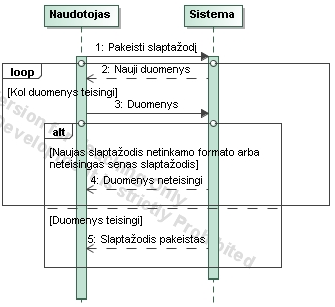
\includegraphics[scale=1, frame]{img/slkeitimas.png}
\caption{Proceso „Slaptažodžio keitimas" sekų diagrama}
\end{figure}


\subsubsection{Visų darbo pasiūlymų sąrašas}
\begin{table}[H]
\caption{Funkciniai reikalavimai. Visų darbo pasiūlymų sąrašas}
\centering
\normalsize
\begin{tabular}{|p{2cm}|p{10cm}|p{3cm}|}
\hline
\rowcolor{gray!30}
\multicolumn{3}{|l|}{\textbf{6. Visų darbų sąrašas}} \\ \hline
\textbf{KODAS}& \multicolumn{1}{m{10cm}|}{\textbf{REIKALAVIMAS}} & \textbf{SVARBA} \\ \hline
FR6.1 & \multicolumn{1}{m{10cm}|}{Visam darbų sąrašui pateikti naudojami puslapiai ( viename puslapyje 10 darbo pasiūlymų).} & Būtinas \\ \hline
FR6.2 & \multicolumn{1}{m{10cm}|}{Visam darbų sąrašui pateikti naudojama lentelė.} & Būtinas \\ \hline
FR6.3 & \multicolumn{1}{m{10cm}|}{Darbo pasiūlymai gali būti rikiuojami pagal visus laukus.} & Būtinas \\ \hline
FR6.4 & \multicolumn{1}{m{10cm}|}{Yra paieškos laukas, kuris ieško konkrečios įvestos frazės.} & Būtinas \\ \hline
FR6.5 & \multicolumn{1}{m{10cm}|}{Jei darbo pasiūlymų sąrašas tuščias, rodomas pranešimas, kad darbo pasiūlymų nėra.} & Būtinas \\ \hline
FR6.6 & \multicolumn{1}{m{10cm}|}{Darbuotojas ir darbdavys negali ištrinti ir redaguoti darbo pasiūlymų.} & Būtinas \\ \hline
FR6.7 & \multicolumn{1}{m{10cm}|}{Administratorius gali ištrinti darbo pasiūlymą.} & Būtinas \\ \hline
FR6.8 & \multicolumn{1}{m{10cm}|}{Šiame sąraše galima  pažymėti darbą, kaip dominantį (žr. FR9), paspaudus ant darbo pažiūrėti detalesnę darbo informaciją (žr. 1.12).} & Būtinas \\ \hline
FR6.9 & \multicolumn{1}{m{10cm}|}{Darbo pasiūlymas yra saugomas 1 mėnesį (30 dienų), po šio termino darbo pasiūlymas automatiškai yra ištrinamas.} & Būtinas \\ \hline
\end{tabular}
\end{table}

\subsubsection{Darbdavio įkeltų darbo pasiūlymų sąrašas}
\begin{table}[H]
\caption{Funkciniai reikalavimai. Darbdavio įkeltų darbo pasiūlymų sąrašas}
\centering
\normalsize
\begin{tabular}{|p{2cm}|p{10cm}|p{3cm}|}
\hline
\rowcolor{gray!30}
\multicolumn{3}{|l|}{\textbf{7. Darbdavio įkeltų darbo pasiūlymų sąrašas}} \\ \hline
\textbf{KODAS}& \multicolumn{1}{m{10cm}|}{\textbf{REIKALAVIMAS}} & \textbf{SVARBA} \\ \hline
FR7.1 & \multicolumn{1}{m{10cm}|}{Visam darbdavio įkeltų darbų sąrašui pateikti naudojami puslapiai ( viename puslapyje 10 darbo pasiūlymų).} & Būtinas \\ \hline
FR7.2 & \multicolumn{1}{m{10cm}|}{Darbdavio įkeltų darbų sąrašui pateikti naudojama lentelė.} & Būtinas \\ \hline
FR7.3 & \multicolumn{1}{m{10cm}|}{Darbo pasiūlymai gali būti redaguojami (žr. 1.11), ištrinami (žr. 1.13), pažiūrima detalesnė informacija (žr. 1.12).} & Būtinas \\ \hline
FR7.4 & \multicolumn{1}{m{10cm}|}{Darbo pasiūlymai gali būti rikiuojami pagal visus laukus.} & Būtinas \\ \hline
FR7.5 & \multicolumn{1}{m{10cm}|}{Yra paieškos laukas, kuris ieško konkrečios įvestos frazės.} & Būtinas \\ \hline
\end{tabular}
\end{table}


\subsubsection{Darbuotoją dominančių darbo pasiūlymų sąrašas}
\begin{table}[H]
\caption{Funkciniai reikalavimai. Darbuotoją dominančių darbo pasiūlymų sąrašas}
\centering
\normalsize
\begin{tabular}{|p{2cm}|p{10cm}|p{3cm}|}
\hline
\rowcolor{gray!30}
\multicolumn{3}{|l|}{\textbf{8. Darbuotoją dominančių darbo pasiūlymų sąrašas}} \\ \hline
\multicolumn{3}{|l|}{Išankstinė sąlyga: naudotojas turi būti prisijungęs prie sistemos}\\ \hline
\textbf{KODAS}& \multicolumn{1}{m{10cm}|}{\textbf{REIKALAVIMAS}} & \textbf{SVARBA} \\ \hline
FR8.1 & \multicolumn{1}{m{10cm}|}{Visam darbuotojų dominančių darbų sąrašui pateikti naudojami puslapiai ( viename puslapyje 10 darbo pasiūlymų).} & Būtinas \\ \hline
FR8.2 & \multicolumn{1}{m{10cm}|}{Darbuotojo dominančių darbų sąrašui pateikti naudojama lentelė.} & Būtinas \\ \hline
FR8.3 & \multicolumn{1}{m{10cm}|}{Rodomi tie darbai, kurie darbuotojo buvo pažymėti, kaip dominantys.} & Būtinas \\ \hline
FR8.4 & \multicolumn{1}{m{10cm}|}{Darbo pasiūlymai gali būti rikiuojami pagal visus laukus.} & Būtinas \\ \hline
FR8.5 & \multicolumn{1}{m{10cm}|}{Yra paieškos laukas, kuris ieško konkrečios įvestos frazės.} & Būtinas \\ \hline
\end{tabular}
\end{table}

\subsubsection{Darbo pasiūlymo pažymėjimas, kaip dominantis}
\begin{table}[H]
\caption{Funkciniai reikalavimai. Darbo pasiūlymo pažymėjimas, kaip dominantis}
\centering
\normalsize
\begin{tabular}{|p{2cm}|p{10cm}|p{3cm}|}
\hline
\rowcolor{gray!30}
\multicolumn{3}{|l|}{\textbf{9. Darbo pasiūlymo pažymėjimas, kaip dominantis}} \\ \hline
\textbf{KODAS}& \multicolumn{1}{m{10cm}|}{\textbf{REIKALAVIMAS}} & \textbf{SVARBA} \\ \hline
FR9.1 & \multicolumn{1}{m{10cm}|}{Dominančius darbo pasiūlymus gali žymėti tik darbuotojai.} & Būtinas \\ \hline
FR9.2 & \multicolumn{1}{m{10cm}|}{Dominantys darbo pasiūlymai yra rodomi dominančių darbų sąraše.} & Būtinas \\ \hline
FR9.3 & \multicolumn{1}{m{10cm}|}{Bendrame sąraše dominantys darbai turi užžymėtą pliusą.} & Būtinas \\ \hline
FR9.4 & \multicolumn{1}{m{10cm}|}{Jei darbo pasiūlymas nebedomina, darbuotojas gali nuimti pliusą.} & Būtinas \\ \hline
\end{tabular}
\end{table}

\subsubsection{Naujo darbo pasiūlymo sukūrimas}
\begin{table}[H]
\caption{Funkciniai reikalavimai. Naujo darbo pasiūlymo sukūrimas}
\centering
\normalsize
\begin{tabular}{|p{2cm}|p{10cm}|p{3cm}|}
\hline
\rowcolor{gray!30}
\multicolumn{3}{|l|}{\textbf{10. Naujo darbo pasiūlymo sukūrimas}} \\ \hline
\textbf{KODAS}& \multicolumn{1}{m{10cm}|}{\textbf{REIKALAVIMAS}} & \textbf{SVARBA} \\ \hline
FR10.1 & \multicolumn{1}{m{10cm}|}{Darbdaviui įvedus darbo pasiūlymo pavadinimą (maksimalus ilgis 250 simbolių) – laukas validuojamas.} & Būtinas \\ \hline
FR10.2 & \multicolumn{1}{m{10cm}|}{Darbdaviui pasirinkus darbo sritį iš pateikto sąrašo - laukas validuojamas.} & Būtinas \\ \hline
FR10.3 & \multicolumn{1}{m{10cm}|}{Darbdaviui pasirinkus darbo pradžios datą – laukas validuojamas.} & Būtinas \\ \hline

\end{tabular}
\end{table}

\begin{table}[H]
\centering
\normalsize
\begin{tabular}{|p{2cm}|p{10cm}|p{3cm}|}
\hline
FR10.4 & \multicolumn{1}{m{10cm}|}{Darbdaviui pasirinkus darbo pradžios datą ankstesnę nei šiandien išvedamas klaidos pranešimas.} & Būtinas \\ \hline
FR10.5 & \multicolumn{1}{m{10cm}|}{Darbdaviui įvedus darbo vietą (maksimalus ilgis 50 simbolių) – laukas validuojamas.} & Būtinas \\ \hline
FR10.6 & \multicolumn{1}{m{10cm}|}{Darbdaviui įvedus algos dydį ( skaičius tarp 0 ir 5000) – laukas validuojamas.} & Būtinas \\ \hline
FR10.7 & \multicolumn{1}{m{10cm}|}{Darbdaviui įvedus darbo trukmę (maksimaliai 50 simbolių) – laukas validuojamas.} & Būtinas \\ \hline
FR10.8 & \multicolumn{1}{m{10cm}|}{Jei kurie nors informacijos laukai yra netinkamo formato arba neįvesti, laukai nuspalvinami raudonai ir išvedamas klaidos pranešimas.} & Būtinas \\ \hline
FR10.9 & \multicolumn{1}{m{10cm}|}{Jei darbdavio suvesta informacija yra tinkama, sukuriamas darbo pasiūlymas.} & Būtinas \\
\hline
FR10.10 & \multicolumn{1}{m{10cm}|}{Jei darbo pasiūlymo išsaugoti nepavyksta, išvedamas klaidos pranešimas ir prašoma pabandyti dar kartą.} & Būtinas \\ \hline
\end{tabular}
\end{table}
17 pav. pateikiama užduoties „Naujo darbo pasiūlymo sukūrimo" sekų diagrama. Joje vaizduojamas pagrindinis  scenarijus kuriant naują darbo pasiūlymą ir taip pat nagrinėjami alternatyvūs scenarijai.
\begin{figure}[H]
\centering
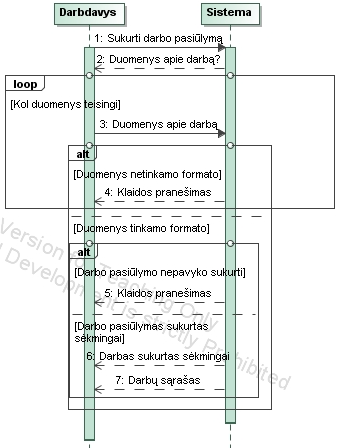
\includegraphics[scale=1, frame]{img/sukurtiDarba.png}
\caption{Proceso „Naujo darbo pasiūlymo sukūrimas" sekų diagrama}
\end{figure}

\subsubsection{Darbo pasiūlymo redagavimas}
\begin{table}[H]
\caption{Funkciniai reikalavimai. Darbo pasiūlymo redagavimas}
\centering
\normalsize
\begin{tabular}{|p{2cm}|p{10cm}|p{3cm}|}
\hline
\rowcolor{gray!30}
\multicolumn{3}{|l|}{\textbf{11. Darbo pasiūlymo redagavimas}} \\ \hline
\textbf{KODAS}& \multicolumn{1}{m{10cm}|}{\textbf{REIKALAVIMAS}} & \textbf{SVARBA} \\ \hline
FR11.1 & \multicolumn{1}{m{10cm}|}{Darbo pasiūlymą gali redaguoti tik jį įkėlęs darbdavys.} & Būtinas \\ \hline
FR11.2 & \multicolumn{1}{m{10cm}|}{Darbo pasiūlymai yra redaguojami darbavio įkeltų darbo pasiūlymų skiltyje.} & Būtinas \\ \hline
FR11.3 & \multicolumn{1}{m{10cm}|}{Paspaudus redaguoti rodoma visa informacija apie darbo pasiūlymą.} & Būtinas \\ \hline
FR11.4 & \multicolumn{1}{m{10cm}|}{Pakeitus informacija tinkama ir išsaugojus, išsaugomas pakeistas darbo pasiūlymas.} & Būtinas \\ \hline
FR11.5 & \multicolumn{1}{m{10cm}|}{Nepavykus išsaugoti pakeitimų, išvedamas klaidos pranešimas.} & Būtinas \\ \hline
\end{tabular}
\end{table}

\subsubsection{Darbo pasiūlymo detali informacija}
\begin{table}[H]
\caption{Funkciniai reikalavimai. Darbo pasiūlymo detali informacija}
\centering
\normalsize
\begin{tabular}{|p{2cm}|p{10cm}|p{3cm}|}
\hline
\rowcolor{gray!30}
\multicolumn{3}{|l|}{\textbf{12. Darbo pasiūlymo detali informacija}} \\ \hline
\multicolumn{3}{|l|}{Išankstinė sąlyga: naudotojas turi būti prisijungęs prie sistemos}\\ \hline
\textbf{KODAS}& \multicolumn{1}{m{10cm}|}{\textbf{REIKALAVIMAS}} & \textbf{SVARBA} \\ \hline
FR12.1 & \multicolumn{1}{m{10cm}|}{Paspaudus ant darbo pasiūlymo matoma darbo informacija ir taip pat matomi darbą pateikusio darbdavio duomenys ( vardas, pavardė ir telefono numeris).} & Būtinas \\ \hline
FR12.2 & \multicolumn{1}{m{10cm}|}{Paspaudus ant darbdavio naudotojas nukreipiamas į langą su darbą įkėlusio darbdavio informacija (žr. FR16).} & Būtinas \\ \hline
\end{tabular}
\end{table}

\subsubsection{Darbo pasiūlymo ištrynimas}
\begin{table}[H]
\caption{Funkciniai reikalavimai. Darbo pasiūlymo ištrynimas}
\centering
\normalsize
\begin{tabular}{|p{2cm}|p{10cm}|p{3cm}|}
\hline
\rowcolor{gray!30}
\multicolumn{3}{|l|}{\textbf{13. Darbo pasiūlymo ištrynimas}} \\ \hline
\multicolumn{3}{|l|}{Išankstinė sąlyga: naudotojas turi būti prisijungęs prie sistemos}\\ \hline
\textbf{KODAS}& \multicolumn{1}{m{10cm}|}{\textbf{REIKALAVIMAS}} & \textbf{SVARBA} \\ \hline
FR13.1 & \multicolumn{1}{m{10cm}|}{Darbo pasiūlymą gali ištrinti tik jį pateikęs darbdavys.} & Būtinas \\ \hline
FR13.2 & \multicolumn{1}{m{10cm}|}{Patvirtinus ištrinimą darbo pasiūlymas yra ištrinamas.} & Būtinas \\ \hline
FR13.3 & \multicolumn{1}{m{10cm}|}{Darbo pasiūlymai yra ištrinami  darbavio įkeltų darbo pasiūlymų skiltyje.} & Būtinas \\ \hline
\end{tabular}
\end{table}

\subsubsection{Naudotojų sąrašas}
\begin{table}[H]
\caption{Funkciniai reikalavimai. Naudotojų sąrašas}
\centering
\normalsize
\begin{tabular}{|p{2cm}|p{10cm}|p{3cm}|}
\hline
\rowcolor{gray!30}
\multicolumn{3}{|l|}{\textbf{14. Naudotojų sąrašas}} \\ \hline
\textbf{KODAS}& \multicolumn{1}{m{10cm}|}{\textbf{REIKALAVIMAS}} & \textbf{SVARBA} \\ \hline
FR14.1 & \multicolumn{1}{m{10cm}|}{Naudotojų sąrašas pateikiamas dviem lentelėmis, vienoje visi registruoti darbuotojai, kitoje registruoti darbdaviai.} & Būtinas \\ \hline
FR14.2 & \multicolumn{1}{m{10cm}|}{Darbdavys ir darbuotojas neturi teisės redaguoti ir ištrinti naudotojo.} & Būtinas \\ \hline
FR14.3 & \multicolumn{1}{m{10cm}|}{Administratorius turi teisę ištrinti naudotoją (žr. FR17).} & Būtinas \\ \hline
FR14.4 & \multicolumn{1}{m{10cm}|}{Paspaudus ant naudotojo rodoma detali informacija (žr. FR16).} & Būtinas \\ \hline
\multicolumn{3}{|l|}{Darbuotojų sąrašas} \\ \hline
FR14.5 & \multicolumn{1}{m{10cm}|}{Darbuotojų sąrašas pateikiamas lentele.} & Būtinas \\ \hline
FR14.6 & \multicolumn{1}{m{10cm}|}{Rodomas naudotojo el.paštas, vardas, pavardė, reitingas} & Būtinas \\ \hline
FR14.7 & \multicolumn{1}{m{10cm}|}{Visam darbuotojo sąrašui pateikti naudojami puslapiai ( viename puslapyje 20 darbuotojų)} & Būtinas \\ \hline
FR14.8 & \multicolumn{1}{m{10cm}|}{Yra paieškos laukas, kuris  ieško konkretaus darbuotojo (pagal įvestą frazę).} & Būtinas \\ \hline
FR14.9 & \multicolumn{1}{m{10cm}|}{Jei darbuotojų sąrašas tuščias, išvedamas pranešimas, kad darbuotojų nėra.} & Būtinas \\ \hline
FR14.10 & \multicolumn{1}{m{10cm}|}{Darbuotojų sąrašas rikiuojamas pagal reitingą mažėjimo tvarka (su didžiausiu reitingu viršuje).} & Būtinas \\ \hline
\multicolumn{3}{|l|}{Darbdavių sąrašas} \\ \hline
FR14.11 & \multicolumn{1}{m{10cm}|}{Darbdavių sąrašas pateikiamas lentele.} & Būtinas \\ \hline
FR14.12 & \multicolumn{1}{m{10cm}|}{Rodomas darbdavio el.paštas, vardas, pavardė, reitingas ir reitingas turimas svetainėje ,,rekvizitai.lt“ (žr. FR15).} & Būtinas \\ \hline
FR14.13 & \multicolumn{1}{m{10cm}|}{Visam darbdavių sąrašui pateikti naudojami puslapiai ( viename puslapyje 20 darbuotojų)} & Būtinas \\ \hline
FR14.14 & \multicolumn{1}{m{10cm}|}{Yra paieškos laukas, kuris ieško konkretaus darbdavio (pagal įvestą frazę).} & Būtinas \\ \hline
FR14.14 & \multicolumn{1}{m{10cm}|}{Jei darbdavių sąrašas tuščias, išvedamas pranešimas, kad darbdavių nėra.} & Būtinas \\ \hline
FR14.14 & \multicolumn{1}{m{10cm}|}{Darbuotojų sąrašas rikiuojamas pagal reitingą mažėjimo tvarka (su didžiausiu reitingu viršuje).} & Būtinas \\ \hline
\end{tabular}
\end{table}


\subsubsection{„rekvizitai.lt“ darbdavio reitingas}
\begin{table}[H]
\caption{Funkciniai reikalavimai. „rekvizitai.lt“ darbdavio reitingas}
\centering
\normalsize
\begin{tabular}{|p{2cm}|p{10cm}|p{3cm}|}
\hline
\rowcolor{gray!30}
\multicolumn{3}{|l|}{\textbf{15. „rekvizitai.lt“ darbdavio reitingas}} \\ \hline
\textbf{KODAS}& \multicolumn{1}{m{10cm}|}{\textbf{REIKALAVIMAS}} & \textbf{SVARBA} \\ \hline
FR15.1 & \multicolumn{1}{m{10cm}|}{Jei darbdavys turi reitingą svetainėje ,,rekvizitai.lt“, rodomas turimas reitingas.} & Būtinas \\ \hline
FR15.2 & \multicolumn{1}{m{10cm}|}{Jei darbdavys reitingo „rekvizitai.lt“ neturi, rodomas „-“.} & Būtinas \\ \hline
FR15.3 & \multicolumn{1}{m{10cm}|}{Reitingai, paimti iš „rekvizitai.lt“, turi būti atnaujinami kas 3 dienas.} & Būtinas \\ \hline
\end{tabular}
\end{table}

\subsubsection{Detali naudotojo informacija}
\begin{table}[H]
\caption{Funkciniai reikalavimai. Detali naudotojo informacija}
\centering
\normalsize
\begin{tabular}{|p{2cm}|p{10cm}|p{3cm}|}
\hline
\rowcolor{gray!30}
\multicolumn{3}{|l|}{\textbf{16. Detali naudotojo informacija}} \\ \hline
\textbf{KODAS}& \multicolumn{1}{m{10cm}|}{\textbf{REIKALAVIMAS}} & \textbf{SVARBA} \\ \hline
FR16.1 & \multicolumn{1}{m{10cm}|}{Rodoma detali naudotojo informacija (el.paštas, vardas, pavardė, statusas, telefono numeris, reitingas ir atsiliepimų sąrašas).} & Būtinas \\ \hline
FR16.2 & \multicolumn{1}{m{10cm}|}{Galima parašyti atsiliepimą apie naudotoją (žr. FR19).} & Būtinas \\ \hline
FR16.3 & \multicolumn{1}{m{10cm}|}{Galima reitinguoti naudotoją (žr. FR18).} & Būtinas \\ \hline
\end{tabular}
\end{table}

\subsubsection{Naudotojo ištrynimas}
\begin{table}[H]
\caption{Funkciniai reikalavimai. Naudotojo ištrynimas}
\centering
\normalsize
\begin{tabular}{|p{2cm}|p{10cm}|p{3cm}|}
\hline
\rowcolor{gray!30}
\multicolumn{3}{|l|}{\textbf{17. Naudotojo ištrynimas}} \\ \hline
\textbf{KODAS}& \multicolumn{1}{m{10cm}|}{\textbf{REIKALAVIMAS}} & \textbf{SVARBA} \\ \hline
FR17.1 & \multicolumn{1}{m{10cm}|}{Naudotoją ištrinti gali tik administratorius.} & Būtinas \\ \hline
FR17.2 & \multicolumn{1}{m{10cm}|}{Paspaudus ištrynimo mygtuką išmetamas langas, kuriame administratorius parašo priežastį, kodėl naudotojas yra šalinimas.} & Būtinas \\ \hline
FR17.3 & \multicolumn{1}{m{10cm}|}{Įrašyta priežastis yra nusiunčiama naudotojui į registracijos metu nurodytą el. paštą.} & Būtinas \\ \hline
FR17.4 & \multicolumn{1}{m{10cm}|}{Užpildžius priežasties lauką ir patvirtinus ištrynimą naudotojas yra ištrinamas.} & Būtinas \\ \hline
FR17.5 & \multicolumn{1}{m{10cm}|}{Ištrynus naudotoją, ištrinami ir visi jam parašyti atsiliepimai ir jo sukurti darbo pasiūlymai.} & Būtinas \\ \hline
\end{tabular}
\end{table}

\subsubsection{Naudotojo reitingavimas}
\begin{table}[H]
\caption{Funkciniai reikalavimai. Naudotojo reitingavimas}
\centering
\normalsize
\begin{tabular}{|p{2cm}|p{10cm}|p{3cm}|}
\hline
\rowcolor{gray!30}
\multicolumn{3}{|l|}{\textbf{18. Naudotojo reitingavimas}} \\ \hline
\textbf{KODAS}& \multicolumn{1}{m{10cm}|}{\textbf{REIKALAVIMAS}} & \textbf{SVARBA} \\ \hline
FR18.1 & \multicolumn{1}{m{10cm}|}{Darbuotoją reitinguoti gali tik darbdavys.} & Būtinas \\ \hline
FR18.2 & \multicolumn{1}{m{10cm}|}{Darbdavį reitinguoti gali tik darbuotojas.} & Būtinas \\ \hline
FR18.3 & \multicolumn{1}{m{10cm}|}{Jei darbdavys reitinguoja darbdavį, išmetamas klaidos pranešimas, kad darbdavius gali reitinguoti tik darbuotojas.} & Būtinas \\ \hline
FR18.4 & \multicolumn{1}{m{10cm}|}{Jei darbuotojas reitinguoja darbuotoją, išmetamas klaidos pranešimas, kad darbuotoją gali reitinguoti tik darbdavys.} & Būtinas \\ \hline
FR18.5 & \multicolumn{1}{m{10cm}|}{Lauke pasirenkamas žvaigždučių skaičius – laukas validuojamas} & Būtinas \\ \hline
FR18.6 & \multicolumn{1}{m{10cm}|}{Reitingas skaičiuojamas imant visų vertinimų vidurkį (2 skaičiai po kablelio)} & Būtinas \\ \hline
FR18.7 & \multicolumn{1}{m{10cm}|}{Jei naudotojas dar nebuvo įvertintas, vietoj reikšmės rašomas „-“.} & Būtinas \\ \hline
\end{tabular}
\end{table}
18 pav. pateikiama užduoties „Naudotojo reitingavimo" sekų diagrama. Joje vaizduojamas pagrindinis naudotojo reitingavimo scenarijus ir taip pat nagrinėjami alternatyvūs scenarijai.
\begin{figure}[H]
\centering
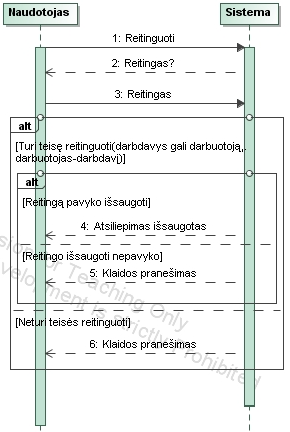
\includegraphics[scale=1, frame]{img/reitingavimas.png}
\caption{Proceso „Naudotojo reitingavimas" sekų diagrama}
\end{figure}

\subsubsection{Atsiliepimų rašymas}
\begin{table}[H]
\caption{Funkciniai reikalavima. Atsiliepimų rašymas}
\centering
\normalsize
\begin{tabular}{|p{2cm}|p{10cm}|p{3cm}|}
\hline
\rowcolor{gray!30}
\multicolumn{3}{|l|}{\textbf{19. Atsiliepimų rašymas}} \\ \hline
\textbf{KODAS}& \multicolumn{1}{m{10cm}|}{\textbf{REIKALAVIMAS}} & \textbf{SVARBA} \\ \hline
FR18.1 & \multicolumn{1}{m{10cm}|}{Darbuotojui atsiliepimą gali rašyti tik darbdavys.} & Būtinas \\ \hline
FR19.2 & \multicolumn{1}{m{10cm}|}{Darbdaviui atsiliepimą gali rašyti tik darbuotojas.} & Būtinas \\ \hline
FR19.3 & \multicolumn{1}{m{10cm}|}{Jei darbdavys rašo atsiliepimą darbdaviui, išmetamas klaidos pranešimas, kad darbdaviui atsiliepimą gali rašyti tik darbuotojas.} & Būtinas \\ \hline
FR19.4 & \multicolumn{1}{m{10cm}|}{Jei darbuotojas rašo atsiliepimą darbuotojui, išmetamas klaidos pranešimas, kad darbuotojui atsiliepimą gali rašyti tik darbdavys.} & Būtinas \\ \hline
FR19.5 & \multicolumn{1}{m{10cm}|}{Įvedus atsiliepimą (maksimalus ilgis 500 simbolių) – laukas validuojamas.} & Būtinas \\ \hline
FR19.6 & \multicolumn{1}{m{10cm}|}{Tinkamai užpildžius laukus ir paspaudus išsaugoti atsiliepimas yra išsaugomas.} & Būtinas \\ \hline
FR19.7 & \multicolumn{1}{m{10cm}|}{Rodoma 60 naujausių atsiliepimų.} & Būtinas \\ \hline
\end{tabular}
\end{table}
19 pav. pateikiama užduoties „Atsiliepimų rašymas" sekų diagrama. Joje vaizduojamas pagrindinis atsiliepimo parašymo scenarijus ir taip pat nagrinėjami alternatyvūs scenarijai.
\begin{figure}[H]
\centering
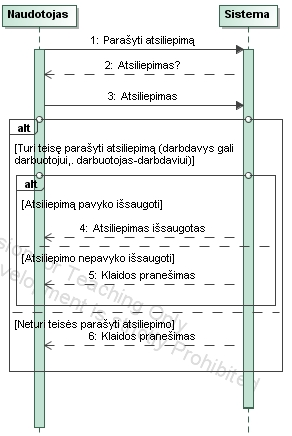
\includegraphics[scale=0.8, frame]{img/atsilras.png}
\caption{Proceso „Atsiliepimų rašymas" sekų diagrama}
\end{figure}

\subsubsection{Atsiliepimų sąrašas}
\begin{table}[H]
\caption{Funkciniai reikalavimai. Atsiliepimų sąrašas}
\centering
\normalsize
\begin{tabular}{|p{2cm}|p{10cm}|p{3cm}|}
\hline
\rowcolor{gray!30}
\multicolumn{3}{|l|}{\textbf{20. Atsiliepimų sąrašas}} \\ \hline
\textbf{KODAS}& \multicolumn{1}{m{10cm}|}{\textbf{REIKALAVIMAS}} & \textbf{SVARBA} \\ \hline
FR20.1 & \multicolumn{1}{m{10cm}|}{Visam atsiliepimų sąrašui pateikti naudojami puslapiai ( viename puslapyje 10 atsiliepimų).} & Būtinas \\ \hline
FR20.2 & \multicolumn{1}{m{10cm}|}{Atsiliepimai surikiuoti pagal datą, naujausi viršuje.} & Būtinas \\ \hline
FR20.3 & \multicolumn{1}{m{10cm}|}{Jei atsiliepimų sąrašas tuščias, išvedamas pranešimas, kad atsiliepimų nėra.} & Būtinas \\ \hline
FR20.4 & \multicolumn{1}{m{10cm}|}{Rodomas atsiliepimą parašiusio naudotojo vardas ir pavardė bei atsiliepimas.} & Būtinas \\ \hline
\end{tabular}
\end{table}

\subsubsection{Kontaktinė informacija}
\begin{table}[H]
\caption{Funkciniai reikalavimai.  Kontaktinė informacija}
\centering
\normalsize
\begin{tabular}{|p{2cm}|p{10cm}|p{3cm}|}
\hline
\rowcolor{gray!30}
\multicolumn{3}{|l|}{\textbf{21. Kontaktinė informacija}} \\ \hline
\textbf{KODAS}& \multicolumn{1}{m{10cm}|}{\textbf{REIKALAVIMAS}} & \textbf{SVARBA} \\ \hline
FR21.1 & \multicolumn{1}{m{10cm}|}{Rodomas sistemos pateikiamas el. pašto adresas} & Būtinas \\ \hline
\end{tabular}
\end{table}

\subsubsection{VIP darbo pasiūlymo pateikimas}
\begin{table}[H]
\caption{Funkciniai reikalavimai. VIP darbo pasiūlymo pateikimas.}
\centering
\normalsize
\begin{tabular}{|p{2cm}|p{10cm}|p{3cm}|}
\hline
\rowcolor{gray!30}
\multicolumn{3}{|l|}{\textbf{22. VIP darbo pasiūlymo pateikimas}} \\ \hline
\textbf{KODAS}& \multicolumn{1}{m{10cm}|}{\textbf{REIKALAVIMAS}} & \textbf{SVARBA} \\ \hline
FR15.1 & \multicolumn{1}{m{10cm}|}{Darbdaviui nurodžius darbo skelbimą ir sumokėjus, jis yra rodomas VIP darbo pasiūlymų skiltyje.} & Būtinas \\ \hline
\end{tabular}
\end{table}
\newpage
%NEFUNKCINIAI REIKALAVIMAI
\subsection{NEFUNKCINIAI REIKALAVIMAI}
2-ame skyriuje pateikiami nefunkciniai reikalavimai bei jų svarba. Aprašoma, kaip sistema turi veikti ir kaip ji turi būti kuriama.
\subsubsection{Vidinių interfeisų reikalavimai}
\begin{table}[H]
\caption{Nefunkciniai reikalavimai. Vidinių interfeisų reikalavimai.}
\centering
\normalsize
\begin{tabular}{|p{2cm}|p{10cm}|p{3cm}|}
\hline
\rowcolor{gray!30}
\multicolumn{3}{|l|}{\centering{\textbf{Vidinių interfeisų reikalavimai}}} \\ \hline
\multicolumn{3}{|l|}{\textbf{OS naudojimo reikalavimai}} \\ \hline
\textbf{KODAS}& \multicolumn{1}{m{10cm}|}{\textbf{REIKALAVIMAS}} & \textbf{SVARBA} \\ \hline
NFR1.1 & \multicolumn{1}{m{10cm}|}{Tinklapis pritaikytas tiek kompiuteriams, tiek mobiliesiems įrenginiams.} & Būtinas \\ \hline
NFR1.2 & \multicolumn{1}{m{10cm}|}{Įrenginyje turi būti bet kuri iš Microsoft Windows (8 arba naujesnė versija), macOS (10.5 arba naujesnė versija), GNU/Linux, iOS, Android operacinių sistemų.} & Būtinas \\ \hline
NFR1.3 & \multicolumn{1}{m{10cm}|}{Puslapis pasiekiamas per visas populiariausias naršykles (Google Chrome, Mozilla Firefox, IE (nuo 8 versijos), Edge, Safari).} & Būtinas \\ \hline
\multicolumn{3}{|l|}{\textbf{Sąveikos su DB reikalavimai}} \\ \hline
NFR2.1 & \multicolumn{1}{m{10cm}|}{Tinklapis turi turėti duomenų bazę, kurioje saugomi naudotojų duomenys, darbo pasiūlymai, reitingai, atsiliepimai bei informacija apie sutartus atlikti darbus.} & Būtinas \\ \hline
NFR2.2 & \multicolumn{1}{m{10cm}|}{Duomenys saugomi reliaciniu būdu, naudojama MySQL duomenų bazių valdymo sistema.} & Būtinas \\ \hline
NFR2.3 & \multicolumn{1}{m{10cm}|}{Naudojama Microsoft Azure SQL Database paslauga.} & Pageidautinas \\ \hline
\multicolumn{3}{|l|}{\textbf{Dokumentų mainų reikalavimai}} \\ \hline
NFR3.1 & \multicolumn{1}{m{10cm}|}{Naudotojų įkeliamos nuotraukos turi būti,.jpg, .png, .bmp formato bei neviršyti 5MB dydžio.} & Būtinas \\ \hline
\multicolumn{3}{|m{10cm}|}{\textbf{Darbo kompiuterių tinkluose reikalavimai}} \\ \hline
NFR4.1 & \multicolumn{1}{m{10cm}|}{Duomenys perduodami naudojant HTTPS protokolą.} & Būtinas \\ \hline
\multicolumn{3}{|l|}{\textbf{Sąveikos su kitomis programomis reikalavimai}} \\ \hline
NFR5.1 & \multicolumn{1}{m{10cm}|}{Tinklapis bus integruotas su rekvizitai.lt.} & Būtinas \\ \hline
\multicolumn{3}{|l|}{\textbf{Programavimo aplinkos reikalavimai}} \\ \hline
NFR6.1 & \multicolumn{1}{m{10cm}|}{Tinklapis kuriamas C\# programavimo kalba, naudojant ASP.NET karkasą.} & Būtinas \\ \hline
NFR6.2 & \multicolumn{1}{m{10cm}|}{Kodo saugojimui ir dalinimuisi naudojama privati Github repositorija.} & Pageidautinas \\ \hline
NFR6.3 & \multicolumn{1}{m{10cm}|}{Naudojama Visual Studio programavimo aplinka.} & Pageidautinas \\ \hline
\end{tabular}
\end{table}

\subsubsection{Veikimo reikalavimai}
\begin{table}[H]
\caption{Nefunkciniai reikalavimai. Veikimo reikalavimai}
\centering
\normalsize
\begin{tabular}{|p{2cm}|p{10cm}|p{3cm}|}
\hline
\rowcolor{gray!30}
\multicolumn{3}{|l|}{\centering{\textbf{Veikimo reikalavimai}}} \\ \hline
\multicolumn{3}{|l|}{\textbf{Vaizdavimo reikalavimai}} \\ \hline
\textbf{KODAS}& \multicolumn{1}{m{10cm}|}{\textbf{REIKALAVIMAS}} & \textbf{SVARBA} \\ \hline
NFR7.1 & \multicolumn{1}{m{10cm}|}{Tinklapis turi būti palaikomas visose populiariausiose naršyklėse (IE (nuo 8 versijos), Edge, Chrome, Safari, Firefox).} & Būtinas \\ \hline
NFR7.2 & \multicolumn{1}{m{10cm}|}{Keičiant naršyklės dydį, tinklapis vaizdą pritaiko automatiškai.} & Būtinas \\ \hline
NFR7.3 & \multicolumn{1}{m{10cm}|}{Data turi būti vaizduojama formatu YYYY-MM-DD, kur YYYY – metai, MM – mėnuo, DD – diena.} & Būtinas \\ \hline
NFR7.4 & \multicolumn{1}{m{10cm}|}{Laikas turi būti vaizduojamas formatu hh:mm, kur hh - valandos, mm - minutės.} & Būtinas \\ \hline
NFR7.5 & \multicolumn{1}{m{10cm}|}{Darbo pavadinimas – ne daugiau 50 simbolių.} & Būtinas \\ \hline
NFR7.6 & \multicolumn{1}{m{10cm}|}{Darbo užmokestis – vienetų tikslumu.} & Būtinas \\ \hline
NFR7.7 & \multicolumn{1}{m{10cm}|}{Reitingai – penkių žvaigdučių skalėje.} & Pageidautinas \\ \hline
\multicolumn{3}{|l|}{\textbf{Skaičiavimo tikslumo reikalavimai}} \\ \hline
NFR8.1 & \multicolumn{1}{m{10cm}|}{Tinklapyje atliekami reitingų skaičiavimai atliekami vieno skaitmens po kablelio tikslumu.} & Būtinas \\ \hline
\multicolumn{3}{|l|}{\textbf{Patikimumo reikalavimai}} \\ \hline
NFR9.1 & \multicolumn{1}{m{10cm}|}{Sistema turi veikti bent 98\% planuoto laiko, t.y. maksimalus leidžiamas sistemos nedarbo laikas yra 28 minutės 48 sekundės per parą.} & Būtinas \\ \hline
\multicolumn{3}{|l|}{\textbf{Robastiškumo reikalavimai}} \\ \hline
NFR10.1 & \multicolumn{1}{m{10cm}|}{Sistemoje turi būti įdiegtos apsaugos priemonės nuo duomenų sugadinimo, praradimo, klaidingų duomenų įvedimo į DB.} & Būtinas \\ \hline
NFR11.1 & \multicolumn{1}{m{10cm}|}{Pranešti naudotojui, jei interneto ryšys nutrūko.} & Pageidautinas \\ \hline
\multicolumn{3}{|l|}{\textbf{Našumo reikalavimai}} \\ \hline
NFR12.1 & \multicolumn{1}{m{10cm}|}{Užklausai įvykdyti turi užtekti ne daugiau nei 5 sekundžių.} & Būtinas \\ \hline
\multicolumn{3}{|m{10cm}|}{\textbf{Darbo kompiuterių tinkluose reikalavimai}} \\ \hline
NFR13.1 & \multicolumn{1}{m{10cm}|}{Svetainės talpinimo (hostingo) planas turi būti parinktas atsižvelgiant į prognozuojamą klientų srautą. Rekomenduojamas duomenų srautas – 50GB/mėn., vieta serveryje -  iki 3 GB.} & Būtinas \\ \hline
NFR13.2 & \multicolumn{1}{m{10cm}|}{Didžiausia leistina tinklapio sistemos apkrova yra 1000 naudotojų, prisijungusių vienu
metu.} & Būtinas \\ \hline
\end{tabular}
\end{table}

\subsubsection{Diegimo reikalavimai}
\begin{table}[H]
\caption{Nefunkciniai reikalavimai. Diegimo reikalavimai.}
\centering
\normalsize
\begin{tabular}{|p{2cm}|p{10cm}|p{3cm}|}
\hline
\rowcolor{gray!30}
\multicolumn{3}{|l|}{\textbf{Diegimo reikalavimai}} \\ \hline
\multicolumn{3}{|l|}{\textbf{Ruošinio reikalavimai}} \\ \hline
\textbf{KODAS}& \multicolumn{1}{m{10cm}|}{\textbf{REIKALAVIMAS}} & \textbf{SVARBA} \\ \hline
& \multicolumn{2}{|l|}{\textbf{Turi būti pateikta: }} \\ \hline
NFR14.1 & \multicolumn{1}{m{10cm}|}{Dokumentacija} & Būtinas \\ \hline
NFR14.2 & \multicolumn{1}{m{10cm}|}{Hostingo prisijungimo duomenys.} & Būtinas \\ \hline
NFR14.3 & \multicolumn{1}{m{10cm}|}{MS Azure prisijungimo duomenys.} & Pageidautinas \\ \hline
\multicolumn{3}{|l|}{\textbf{Instaliavimo reikalavimai}} \\ \hline
NFR15.1 & \multicolumn{1}{m{10cm}|}{Apsilankęs internetiniame pusalpyje, vartotojas privalo sutikti su slapukų naudojimo sąlygomis.} & Būtinas \\ \hline
\multicolumn{3}{|l|}{\textbf{Pradinio DB kaupimo reikalavimai}} \\ \hline
NFR16.1 & \multicolumn{1}{m{10cm}|}{Turi būti sukurtos lentelės.} & Būtinas \\ \hline
NFR16.2 & \multicolumn{1}{m{10cm}|}{Naudotojų lentelėje turi būti administratoriaus duomenys.} & Būtinas \\ \hline
\multicolumn{3}{|l|}{\textbf{Sistemos įsisavinamumo reikalavimai}} \\ \hline
NFR17.1 & \multicolumn{1}{m{10cm}|}{Sistema turi funkcionuoti dvejomis kalbomis: lietuvių ir anglų.} & Būtinas \\ \hline
NFR17.2 & \multicolumn{1}{m{10cm}|}{Negali būti klaidinančių nuorodų.} & Būtinas \\ \hline
NFR17.3 & \multicolumn{1}{m{10cm}|}{Ikonos turi atspindėti mygtuko panaudojimą.} & Būtinas \\ \hline
\end{tabular}
\end{table}
\subsubsection{Aptarnavimo ir priežiūros reikalavimai}
\begin{table}[H]
\caption{Nefunkciniai reikalavimai. Aptarnavimo ir priežiūros reikalavimai.}
\centering
\normalsize
\begin{tabular}{|p{2cm}|p{10cm}|p{3cm}|}
\hline
\rowcolor{gray!30}
\multicolumn{3}{|l|}{\textbf{Aptarnavimo ir priežiūros reikalavimai}} \\ \hline
NFR18.1 & \multicolumn{1}{m{10cm}|}{Atsiradęs naujas funkcionalumas turi būti įdiegtas per 5 darbo dienas.} & Būtinas \\ \hline
NFR18.2 & \multicolumn{1}{m{10cm}|}{Rasta klaida turi būti ištaisyta per 2 darbo dienas.} & Būtinas \\ \hline
NFR18.3 & \multicolumn{1}{m{10cm}|}{Į naudotojo laiškus su pastebėjimais ir skundais atsakyti reikia per 3 darbo dienas.} & Pageidautinas \\ \hline
NFR18.4 & \multicolumn{1}{m{10cm}|}{Jei dėl planuojamo atnaujinimo reikės trumpam sustabdyti sistemos veiklą, naudotojai turi būti iš anksto įspėti ne mažiau nei prieš 24 val.} & Pageidautinas \\ \hline
\end{tabular}
\end{table}


\subsubsection{Tiražuojamumo reikalavimai}
\begin{table}[H]
\caption{Nefunkciniai reikalavimai. Tiražuojamumo reikalavimai.}
\centering
\normalsize
\begin{tabular}{|p{2cm}|p{10cm}|p{3cm}|}
\hline
\rowcolor{gray!30}
\multicolumn{3}{|l|}{\textbf{Tiražuojamumo reikalavimai}} \\ \hline
NFR19.1 & \multicolumn{1}{m{10cm}|}{Internetinė svetainė turi veikti bet kuriame įrenginyje, kuris turi naršyklę ir interneto ryšį.} & Būtinas \\ \hline
\end{tabular}
\end{table}
\subsubsection{Apsaugos reikalavimai}
\begin{table}[H]
\caption{Nefunkciniai reikalavimai. Apsaugos reikalavimai.}
\centering
\normalsize
\begin{tabular}{|p{2cm}|p{10cm}|p{3cm}|}
\hline
\rowcolor{gray!30}
\multicolumn{3}{|l|}{\textbf{Apsaugos reikalavimai}} \\ \hline
NFR20.1 & \multicolumn{1}{m{10cm}|}{Naudotojui prisijungiant prie sistemos vykdoma jo identifikacija.} & Būtinas \\ \hline
NFR20.2 & \multicolumn{1}{m{10cm}|}{Duomenų bazėje saugomas slaptažodžių maišos kodas, o ne pats slaptažodis.} & Būtinas \\ \hline
NFR20.3 & \multicolumn{1}{m{10cm}|}{Atsarginės DB kopijos daromos ne rečiau nei kas savaitę.} & Būtinas \\ \hline
NFR20.4 & \multicolumn{1}{m{10cm}|}{Jei naudotojas neaktyvus ilgiau nei 30 minučių, jis turi būti automatiškai atjungiamas nuo sistemos.} & Būtinas \\ \hline
\end{tabular}
\end{table}
\subsubsection{Juridiniai reikalavimai}
\begin{table}[H]
\caption{Nefunkciniai reikalavimai. Juridiniai reikalavimai.}
\centering
\normalsize
\begin{tabular}{|p{2cm}|p{10cm}|p{3cm}|}
\hline
\rowcolor{gray!30}
\multicolumn{3}{|l|}{\textbf{Juridiniai reikalavimai}} \\ \hline
NFR21.1 & \multicolumn{1}{m{10cm}|}{Kuriant sistemą projekto komanda neturi naudotis nelegalia programine įranga.} & Būtinas \\ \hline
NFR21.2 & \multicolumn{1}{m{10cm}|}{Naudotojas registracijos metu turi sutikti su naudojimosi sąlygomis.} & Būtinas \\ \hline
NFR21.3 & \multicolumn{1}{m{10cm}|}{Internetinėje svetainėje turi būti galimybė peržiūrėti naudojimosi sąlygas.} & Būtinas \\ \hline
\end{tabular}
\end{table}

\newpage

%VARTOTOJO SĄSAJOS REIKALAVIMAI
\subsection{VARTOTOJO SĄSAJOS REIKALAVIMAI}
3 skyriuje pateikiami vartotojo sąsajos reikalavimai, kuriuose pateikiama informaciją apie sistemos grafinį vaizdą, kurį mato vartotojas. Nagrinėjami naudotojui matomi puslapiai, ikonos, simboliai bei mygtukai, pavaizduoti prototipuose (žr. 1 priedas). Taip pat aprašomos jų funkcijos, paskirtys bei svarbumas. 

\subsubsection{Dalykinės srities metaforos reikalavimai}
\begin{table}[H]
\caption{Vartotojo interfeiso reikalavimai. Dalykinės srities metaforos reikalavimai.}
\centering
\normalsize
\begin{tabular}{|p{2cm}|p{10cm}|p{3cm}|}
\hline
\rowcolor{gray!30}
\multicolumn{3}{|l|}{\textbf{1.	Dalykinės srities metaforos reikalavimai}} \\ \hline
\textbf{KODAS}& \multicolumn{1}{m{10cm}|}{\textbf{REIKALAVIMAS}} & \textbf{SVARBA} \\ \hline
VIR1.1 & \multicolumn{1}{m{10cm}|}{Puslapio perkrovimas ir pagrindinio puslapio atvertimas yra vaizduojamas puslapio logotipu – dvi viena kitą spaudžiančios rankos.} & Būtinas \\ \hline
VIR1.2 & \multicolumn{1}{m{10cm}|}{Darbo pasiūlymo ištrynimas yra vaizduojamas šiukšlių dėžės simboliu.} & Pageidautinas \\ \hline
VIR1.3 & \multicolumn{1}{m{10cm}|}{Darbo pasiūlymo redagavimas yra rodomas pieštuko simboliu.} & Pageidautinas \\ \hline
VIR1.4 & \multicolumn{1}{m{10cm}|}{Darbo pasiūlymo paieška rodoma padidinamo stiklo simboliu.} & Pageidautinas \\ \hline
VIR1.5 & \multicolumn{1}{m{10cm}|}{Darbo pasiūlymo įterpimas į asmeninį darbų sąrašą yra vaizduojamas „+“ pavidalu.} & Pageidautinas \\ \hline
VIR1.6 & \multicolumn{1}{m{10cm}|}{Darbo pasiūlymo sukūrimo patvirtinimas yra vaizduojamas varnele.} & Pageidautinas \\ \hline
VIR1.7 & \multicolumn{1}{m{10cm}|}{Darbuotojų ir darbdavių reitingas yra vaizduojamas žvaigždutėmis nuo vienos iki penkių.} & Būtinas \\ \hline
\end{tabular}
\end{table}

\subsubsection{Užduočių reikalavimai}
\begin{table}[H]
\caption{Vartotojo interfeiso reikalavimai. Užduočių reikalavimai.}
\centering
\normalsize
\begin{tabular}{|p{2cm}|p{10cm}|p{3cm}|}
\hline
\rowcolor{gray!30}
\multicolumn{3}{|l|}{\textbf{2.	Užduočių reikalavimai}} \\ \hline
\textbf{KODAS}& \multicolumn{1}{m{10cm}|}{\textbf{REIKALAVIMAS}} & \textbf{SVARBA} \\ \hline
\multicolumn{3}{|l|}{\textbf{Neprisiregistravusio naudotojo sąsajos užduotys}} \\ \hline
VIR2.1 & \multicolumn{1}{m{10cm}|}{Prisiregistruoti prie aplikacijos.} & Būtinas \\ \hline
VIR2.2 & \multicolumn{1}{m{10cm}|}{Susipažinti su aplikacijos veiklomis.} & Būtinas \\ \hline
\multicolumn{3}{|l|}{\textbf{Darbdavio sąsajos užduotys}} \\ \hline
VIR3.1 & \multicolumn{1}{m{10cm}|}{Prisijungti prie savo paskyros.} & Būtinas \\ \hline
VIR3.2 & \multicolumn{1}{m{10cm}|}{Redaguoti savo prisijungimo slaptažodį.} & Būtinas \\ \hline
\end{tabular}
\end{table}

\begin{table}[H]
\centering
\normalsize
\begin{tabular}{|p{2cm}|p{10cm}|p{3cm}|}
\hline
VIR3.3 & \multicolumn{1}{m{10cm}|}{Atsijungti nuo savo paskyros.} & Būtinas \\ \hline
VIR3.4 & \multicolumn{1}{m{10cm}|}{Pridėti darbo pasiūlymą.} & Būtinas \\ \hline
VIR3.5 & \multicolumn{1}{m{10cm}|}{Koreguoti darbo pasiūlymą.} & Būtinas \\ \hline
VIR3.6 & \multicolumn{1}{m{10cm}|}{Ištrinti darbo pasiūlymą.} & Būtinas \\ \hline
VIR3.7 & \multicolumn{1}{m{10cm}|}{Peržvelgti visų puslapyje patalpintų darbų sąrašą.} & Būtinas \\ \hline
VIR3.8 & \multicolumn{1}{m{10cm}|}{Peržvelgti savo įkeltų darbų sąrašą.} & Būtinas \\ \hline
VIR3.9 & \multicolumn{1}{m{10cm}|}{Peržiūrėti TOP darbdavių ir darbuotojų sąrašus.} & Būtinas \\ \hline
VIR3.10 & \multicolumn{1}{m{10cm}|}{Reitinguoti darbuotojus.} & Būtinas \\ \hline
VIR3.11 & \multicolumn{1}{m{10cm}|}{Palikti atsiliepimą darbuotojui.} & Būtinas \\ \hline
VIR3.12 & \multicolumn{1}{m{10cm}|}{Peržiūrėti savo reitingą (vidurkis visų gautų reitingų)} & Būtinas \\ \hline
VIR3.13 & \multicolumn{1}{m{10cm}|}{Peržiūrėti gautus atsiliepimus.} & Būtinas \\ \hline
VIR3.14 & \multicolumn{1}{m{10cm}|}{Atsakyti į atsiliepimus.} & Būtinas \\ \hline
\multicolumn{3}{|l|}{\textbf{Darbuotojo sąsajos užduotys }} \\ \hline
VIR4.1 & \multicolumn{1}{m{10cm}|}{Prisijungti prie savo paskyros.} & Būtinas \\ \hline
VIR4.2 & \multicolumn{1}{m{10cm}|}{Redaguoti savo prisijungimo slaptažodį.} & Būtinas \\ \hline
VIR4.3 & \multicolumn{1}{m{10cm}|}{Atsijungti nuo savo paskyros.} & Būtinas \\ \hline
VIR4.4 & \multicolumn{1}{m{10cm}|}{Peržvelgti visų puslapyje patalpintų darbų sąrašą.} & Būtinas \\ \hline
VIR4.5 & \multicolumn{1}{m{10cm}|}{Susirasti darbą pagal norimą kriterijų.} & Būtinas \\ \hline
VIR4.6 & \multicolumn{1}{m{10cm}|}{Pridėti patikusį darbą į asmeninį sąrašą.} & Būtinas \\ \hline
VIR4.7 & \multicolumn{1}{m{10cm}|}{Peržiūrėti TOP darbdavių ir darbuotojų sąrašus.} & Būtinas \\ \hline
VIR4.8 & \multicolumn{1}{m{10cm}|}{Reitinguoti darbdavius.} & Būtinas \\ \hline
VIR4.9 & \multicolumn{1}{m{10cm}|}{Palikti atsiliepimą darbdaviui.} & Būtinas \\ \hline
VIR4.10 & \multicolumn{1}{m{10cm}|}{Peržiūrėti savo reitingą (vidurkis visų gautų reitingų)} & Būtinas \\ \hline
VIR4.11& \multicolumn{1}{m{10cm}|}{Peržiūrėti gautus atsiliepimus.} & Būtinas \\ \hline
VIR4.12 & \multicolumn{1}{m{10cm}|}{Atsakyti į atsiliepimus.} & Būtinas \\ \hline
\multicolumn{3}{|l|}{\textbf{Administratoriaus sąsajos reikalavimai}} \\ \hline
VIR5.1 & \multicolumn{1}{m{10cm}|}{Trinti šiukšles (akivaizdžiai netikrus darbo pasiūlymus ar jau nebegaliojančius).} & Būtinas \\ \hline
VIR5.2 & \multicolumn{1}{m{10cm}|}{Kurti sąrašus duomenų bazėje.} & Būtinas \\ \hline
VIR5.3 & \multicolumn{1}{m{10cm}|}{Atnaujinti tinklapį.} & Būtinas \\ \hline
VIR5.4 & \multicolumn{1}{m{10cm}|}{Blokuoti naudotojus.} & Būtinas \\ \hline
VIR5.5 & \multicolumn{1}{m{10cm}|}{Taisyti aplikacijos klaidas.} & Būtinas \\ \hline
\multicolumn{3}{|l|}{\textbf{Bendri reikalavimai}} \\ \hline
VIR6.1 & \multicolumn{1}{m{10cm}|}{Puslapio viršuje visada esantis meniu.} & Būtinas \\ \hline
VIR6.2 & \multicolumn{1}{m{10cm}|}{Teksto įvedimo formų laukai.} & Būtinas \\ \hline
VIR6.3 & \multicolumn{1}{m{10cm}|}{Ikonos.} & Būtinas \\ \hline
VIR6.4 & \multicolumn{1}{m{10cm}|}{Puslapio dešiniame kampe visada esantis atsijungimo mygtukas.} & Būtinas \\ \hline
\end{tabular}
\end{table}

\subsubsection{Užduočių formulavimo kalbos reikalavimai}
\begin{table}[H]
\caption{Vartotojo interfeiso reikalavimai. Užduočių formulavimo kalbos reikalavimai}
\centering
\normalsize
\begin{tabular}{|p{2cm}|p{10cm}|p{3cm}|}
\hline
\rowcolor{gray!30}
\multicolumn{3}{|l|}{\textbf{3.	Užduočių formulavimo kalbos reikalavimai}} \\ \hline
\textbf{KODAS}& \multicolumn{1}{m{10cm}|}{\textbf{REIKALAVIMAS}} & \textbf{SVARBA} \\ \hline
 & \multicolumn{2}{|l|}{Įrankiai skirti naudotojui naudotis aplikacija} \\ \hline
VIR7.1 & \multicolumn{1}{m{10cm}|}{Grafinis meniu – vartotojo sąsaja su programėle.} & Būtinas \\ \hline
VIR7.2 & \multicolumn{1}{m{10cm}|}{Mygtukai – naudojami siekiant patekti į kitus tinklapio langus.} & Būtinas \\ \hline
VIR7.3 & \multicolumn{1}{m{10cm}|}{Ikonos – interfeise naudojamos piktogramos.} & Būtinas \\ \hline
VIR7.4 & \multicolumn{1}{m{10cm}|}{Įvedimo laukai – naudojami naudotojui įvesti tekstinius duomenis.} & Būtinas \\ \hline
VIR7.5 & \multicolumn{1}{m{10cm}|}{Patvirtinimo langai - langai prašantys naudotojo dar kartą patvirtinti tam tikrą svarbų veiksmą.} & Būtinas \\ \hline
VIR8 & \multicolumn{1}{m{10cm}|}{Naudotojo prisijungimo vardas turi būti validus el.paštas.} & Būtinas \\ \hline
VIR9.1 & \multicolumn{1}{m{10cm}|}{Naudotojo slaptažodis turi būti sudarytas iš raidžių (didžiųjų ir mažųjų), skaitmenų ir specialių simbolių.} & Būtinas \\ \hline
VIR9.2 & \multicolumn{1}{m{10cm}|}{Slaptažodis turi būti ne trumpesnis nei 8 simboliai.} & Būtinas \\ \hline
VIR10 & \multicolumn{1}{m{10cm}|}{Naudotojo el.paštas turi būti įvestas tinkama forma (pvz.: vardaspavarde@paštas.lt)} & Būtinas \\ \hline
\end{tabular}
\end{table}

\subsubsection{Užduočių formulavimo protokolo reikalavimai}
\begin{table}[H]
\caption{Vartotojo interfeiso reikalavimai. Užduočių formulavimo protokolo reikalavimai}
\centering
\normalsize
\begin{tabular}{|p{2cm}|p{10cm}|p{3cm}|}
\hline
\rowcolor{gray!30}
\multicolumn{3}{|l|}{\textbf{4.	Užduočių formulavimo protokolo reikalavimai}} \\ \hline
\textbf{KODAS}& \multicolumn{1}{m{10cm}|}{\textbf{REIKALAVIMAS}} & \textbf{SVARBA} \\ \hline
\multicolumn{3}{|l|}{\textbf{Prisiregistravimas prie sistemos (žr. 1 Priedas, pav. 46)}} \\ \hline
VIR11.1 & \multicolumn{1}{m{10cm}|}{Norėdamas prisiregistruoti naudotojas turi paspausti viršutiniame dešiname kampe esantį mygtuką „Registruotis“. Paspaudus mygtuką išmetamas registracijos langas, kuriame reikalaujama suvesti naudotojo duomenis (el. paštas, slaptažodis, vardas, pavardė, telefono numeris ir kategorija (darbdavys/darbuotojas))} & Būtinas \\ \hline
VIR11.2 & \multicolumn{1}{m{10cm}|}{Paspaudus mygtuką „Registruotis“ registracijos lange tikrinama ar duomenys suvesti teisingai ir ar tokio naudotojo dar nėra duomenų bazėje, jei viskas gerai, naudotojas prijungiamas prie paskyros. Kitu atveju į ekraną išmetamos žinutės prie tų laukų, kurie yra suvesti klaidingai.} & Būtinas \\ \hline
\end{tabular}
\end{table}

\begin{table}[H]
\centering
\normalsize
\begin{tabular}{|p{2cm}|p{10cm}|p{3cm}|}
\hline
\multicolumn{3}{|l|}{\textbf{Prisijungimas prie sistemos  (žr. 1 Priedas, pav. 47)}} \\ \hline
VIR12.1 & \multicolumn{1}{m{10cm}|}{Prisijungti gali tik registruotas naudotojas. Tai padaryti gali dešiniame viršutiniame kampe paspaudęs mygtuką  „Prisijungti“ ir išvestame lange suvedęs savo prisijungimo duomenis (el.paštą, slaptažodį)} & Būtinas \\ \hline
VIR12.2 & \multicolumn{1}{m{10cm}|}{Paspaudus tvirtinantį prisijungimą  mygtuką  „Prisijungti“ duomenys yra patikrinami duomenų bazėje ir, jei viskas teisinga, naudotojas yra prijungiamas. Jei prisijungimas klaidingas, naudotojui išmetama žinutė, kad prijungimas nepavyko.} & Būtinas \\ \hline
VIR12.3 & \multicolumn{1}{m{10cm}|}{Prisijungiant galima pažymėti varnele prie „Prisiminti mane“ ir kitą kartą naudotojas bus prijungiamas automatiškai, nevedant duomenų iš naujo.} & Būtinas \\ \hline
\multicolumn{3}{|l|}{\textbf{Pamirštas slaptažodis}} \\ \hline
VIR13.1 & \multicolumn{1}{m{10cm}|}{Pamiršus slaptažodį galima paspausti ant mygtuko „Pamiršau slaptažodį“. Atsiradusiame lange reikia įvesti el.paštą, kuriuo naudotojas prisijungia. (žr. 1 Priedas, pav. 48)} & Būtinas \\ \hline
VIR13.2 & \multicolumn{1}{m{10cm}|}{Sistema radusi tokį el.paštą duomenų bazėje išsiunčia linką nurodytu el.pašto adresu nukreipiančiu į formą leidžiančią nusistatyti naują slaptažodį. (žr. 1 Priedas, pav. 49)} & Būtinas \\ \hline
\multicolumn{3}{|l|}{\textbf{Pagrindinis juostinis meniu}} \\ \hline
VIR14.1 & \multicolumn{1}{m{10cm}|}{Vaizduojamas viršutinėje puslapio dalyje, matomas kiekviename pasirinkimų lange.} & Būtinas \\ \hline
VIR14.2 & \multicolumn{1}{m{10cm}|}{Kairiame kampe vaizduojamas aplikacijos logotipas ir pavadinimas „Workly“.} & Būtinas \\ \hline
VIR14.3 & \multicolumn{1}{m{10cm}|}{Dešiniame kampe rodomas naudotojo el.paštas, kuris nukreipia į profilį, kuriame galima rasti asmeninius atsiliepimus, prisijungimo informaciją, ir atsijungimo mygtukas „Atsijungti“.} & Būtinas \\ \hline
VIR14.4 & \multicolumn{1}{m{10cm}|}{"Kontaktai" - atverčiami kontaktai norint susisieti su administracija kilus klausimui.  (žr. 1 Priedas, pav. 50)} & Būtinas \\ \hline
VIR14.5 & \multicolumn{1}{m{10cm}|}{„Naudotojų sąrašas“ – pasirinkimas leidžiantis pamatyti geriausių darbuotojų ir darbdavių sąrašus.} & Būtinas \\ \hline
VIR14.6 & \multicolumn{1}{m{10cm}|}{„Darbo pasiūlymai“ – atidaro tinklapyje sukeltų darbų pasiūlymų sąrašą.} & Būtinas \\ \hline
VIR14.7 & \multicolumn{1}{m{10cm}|}{„Dominantys darbo pasiūlymai“ – atverčia asmeninį sudominusių darbų sąrašą (rodomas tik darbuotojui).} & Būtinas \\ \hline
VIR14.7 & \multicolumn{1}{m{10cm}|}{„Įkelti darbo pasiūlymai“ – atverčia asmeninį patalpintų darbų sąrašą (rodomas tik darbdaviui).} & Būtinas \\ \hline
\end{tabular}
\end{table}

\begin{table}[H]
\centering
\normalsize
\begin{tabular}{|p{2cm}|p{10cm}|p{3cm}|}
\hline
\multicolumn{3}{|l|}{\textbf{„Workly“/logotipas}} \\ \hline
VIR15 & \multicolumn{1}{m{10cm}|}{Paspaudus, pateikiama informacija apie tinklapį. (žr. 1 Priedas, pav. 51, pav. 52, pav. 53)} & Būtinas \\ \hline
\multicolumn{3}{|l|}{\textbf{„Naudotojų sąrašas“ (žr. 1 Priedas, pav. 54)}} \\ \hline
VIR16.1 & \multicolumn{1}{m{10cm}|}{Pateikia darbuotojų ir darbdavių sąrašus su jų reitingais nuo geriausio.} & Būtinas \\ \hline
VIR16.2 & \multicolumn{1}{m{10cm}|}{Paspaudus ant sudominusio darbdavio/darbuotojo galima pamatyti jo atsiliepimus. Paspaudus ant darbdavio galima matyti jo siūlomus darbus. (žr. 1 Priedas, pav. 55 ir pav. 56)} & Būtinas \\ \hline
VIR16.3 & \multicolumn{1}{m{10cm}|}{Paspaudus ant padidinamo stiklo aktyvuojamas įvesties langas, kuriame galima ieškoti darbo suvedant tai, ko ieškoma.} & Būtinas \\ \hline
\multicolumn{3}{|l|}{\textbf{„Darbo pasiūlymai“ (žr. 1 Priedas, pav. 57 ir pav. 58)}} \\ \hline
VIR17.1 & \multicolumn{1}{m{10cm}|}{Pateikiamas pilnas darbų sąrašas su kriterijais (darbo pavadinimas, sritis, darbo pradžia, vieta, atlyginimas, trukmė)} & Būtinas \\ \hline
VIR17.2 & \multicolumn{1}{m{10cm}|}{Paspaudus ant padidinamo stiklo aktyvuojamas įvesties langas, kuriame galima ieškoti darbo suvedant tai, ko ieškoma.} & Būtinas \\ \hline
VIR17.3 & \multicolumn{1}{m{10cm}|}{Paspaudus ant darbo pasiūlymo išmetama informacija apie darbdavį, parodomi jo kontaktai, el. paštas. (žr. 1 Priedas, pav. 59)} & Būtinas \\ \hline
\multicolumn{3}{|l|}{\textbf{Dominantys darbo pasiūlymai (pasiekiami tik  darbuotojui) (žr. 1 Priedas, pav. 60)}} \\ \hline
VIR18.1 & \multicolumn{1}{m{10cm}|}{Pateikiami darbai, kuriais darbuotojas susidomėjo anksčiau pažymėdamas „+“ simbolį.} & Būtinas \\ \hline
VIR18.2 & \multicolumn{1}{m{10cm}|}{Paspaudus ant padidinamo stiklo aktyvuojamas įvesties langas, kuriame galima ieškoti darbo suvedant tai, ko ieškoma.} & Būtinas \\ \hline
\multicolumn{3}{|l|}{\textbf{Įkelti darbo pasiūlymai (pasiekiami tik darbdaviui) (žr. 1 Priedas, pav. 61)}} \\ \hline
VIR19.1 & \multicolumn{1}{m{10cm}|}{Pateikiami asmeniniai darbdavio įkelti darbo pasiūlymai.} & Būtinas \\ \hline
VIR19.2 & \multicolumn{1}{m{10cm}|}{Paspaudus ant pieštuko simbolio prie darbo pasiūlymo galima jį redaguoti, visi laukai su informacija tampa aktyviais tekstiniai laukais. Paredagavus pasiūlymą ir paspaudus „Išsaugoti“ iššoks lentelė prašanti redagavimo patvirtinimo. (žr. 1 Priedas, pav. 62)} & Būtinas \\ \hline
VIR19.3 & \multicolumn{1}{m{10cm}|}{Paspaudus ant šiukšlių dėžės simbolio galima ištrinti  darbo pasiūlymą. Paspaudus šį simbolį iššoks patvirtinimo prašanti lentelė.} & Būtinas \\ \hline
VIR19.4 & \multicolumn{1}{m{10cm}|}{Paspaudus ant padidinamo stiklo aktyvuojamas įvesties langas, kuriame galima ieškoti darbo suvedant tai, ko ieškoma.} & Būtinas \\ \hline
\end{tabular}
\end{table}

\begin{table}[H]
\centering
\normalsize
\begin{tabular}{|p{2cm}|p{10cm}|p{3cm}|}
\hline
VIR19.5 & \multicolumn{1}{m{10cm}|}{Paspaudus ant "Įkelti darbo pasiūlymą" yra atverčiama forma, darbo pasiūlymo patalpinimui (žr. 1 Priedas, pav. 63 )} & Būtinas \\ \hline

\multicolumn{3}{|l|}{\textbf{Šoninė juosta}} \\ \hline
VIR20.1 & \multicolumn{1}{m{10cm}|}{Matoma dešinėje sistemos pusėje, matoma kiekviename pasirinkimų lange.} & Būtinas \\ \hline
VIR20.2 & \multicolumn{1}{m{10cm}|}{Viršutinėje juostos dalyje po naudotojo el.pašto ir „Atsijungti“ mygtuko rodomas naudotojo reitingas 5 žvaigždučių principu, kurios atvaizduoja reitingą rodomą šalia.} & Būtinas \\ \hline
\multicolumn{3}{|l|}{\textbf{„El. paštas“ (žr. 1 Priedas, pav. 64)}} \\ \hline
VIR21.1 & \multicolumn{1}{m{10cm}|}{Paspaudus išmetama informacija apie naudotoją.} & Būtinas \\ \hline
VIR21.2 & \multicolumn{1}{m{10cm}|}{Paspaudus išmetami visi turimi atsiliepimai parašyti kitų naudotojų.} & Būtinas \\ \hline
VIR21.3 & \multicolumn{1}{m{10cm}|}{Paspaudus ant mygtuko „Pakeisti slaptažodį“ naudotojui išmetama forma, kurioje galima pasikeisti savo prisijungimo slaptažodį. (žr. 1 Priedas, pav. 65)} & Būtinas \\ \hline
\end{tabular}
\end{table}

\subsubsection{Pranešimo formulavimo reikalavimai}
\begin{table}[H]
\caption{Vartotojo interfeiso reikalavimai. Pranešimo formulavimo reikalavimai}
\centering
\normalsize
\begin{tabular}{|p{2cm}|p{10cm}|p{3cm}|}
\hline
\rowcolor{gray!30}
\multicolumn{3}{|l|}{\textbf{5.	Pranešimo formulavimo reikalavimai}} \\ \hline
\textbf{KODAS}& \multicolumn{1}{m{10cm}|}{\textbf{REIKALAVIMAS}} & \textbf{SVARBA} \\ \hline
VIR22 & \multicolumn{1}{m{10cm}|}{Pranešimai turi būti parašyti laikantis gramatikos ir skyrybos taisyklių.} & Būtinas \\ \hline
VIR23 & \multicolumn{1}{m{10cm}|}{Pranešimai turi būti aiškūs, suprantami ir vienareikšmiški. Aprašo tik tą sritį, dėl kurios yra išmetami naudotojui.} & Būtinas \\ \hline
VIR24 & \multicolumn{1}{m{10cm}|}{Patvirtinimai turi būti aiškūs, suprantami ir vienareikšmiški. Klausia tik patvirtinimo reikalingo užduočiai užbaigti arba nutraukti.} & Būtinas \\ \hline
\end{tabular}
\end{table}

\subsubsection{Interfeiso darnos ir standartizavimo reikalavimai}
\begin{table}[H]
\caption{Vartotojo interfeiso reikalavimai. Interfeiso darnos ir standartizavimo reikalavimai}
\centering
\normalsize
\begin{tabular}{|p{2cm}|p{10cm}|p{3cm}|}
\hline
\rowcolor{gray!30}
\multicolumn{3}{|l|}{\textbf{6.	Interfeiso darnos ir standartizavimo reikalavimai}} \\ \hline
\textbf{KODAS}& \multicolumn{1}{m{10cm}|}{\textbf{REIKALAVIMAS}} & \textbf{SVARBA} \\ \hline
VIR25 & \multicolumn{1}{m{10cm}|}{Vartotojo interfeisas turi būti pritaikytas tiek Android OS, tiek Mac OS X, tiek Microsoft Windows ar GNU/Linux operacinėms sistemoms.} & Būtinas \\ \hline
\end{tabular}
\end{table}

\begin{table}[H]
\centering
\normalsize
\begin{tabular}{|p{2cm}|p{10cm}|p{3cm}|}
\hline
VIR26 & \multicolumn{1}{m{10cm}|}{Visi grafiniai objektai turi derėti tarpusavyje. Visi mygtukai, lentelės pranešimai, ikonos derančios išvaizdos.} & Būtinas \\ \hline
VIR27 & \multicolumn{1}{m{10cm}|}{Tinklapyje naudojamos vienos paletės spalvos ir lengvai įskaitomas šriftas.} & Būtinas \\ \hline
\end{tabular}
\end{table}

\subsubsection{Interfeiso individualizavimo reikalavimai}
\begin{table}[H]
\caption{Vartotojo interfeiso reikalavimai. Interfeiso individualizavimo reikalavimai}
\centering
\normalsize
\begin{tabular}{|p{2cm}|p{10cm}|p{3cm}|}
\hline
\rowcolor{gray!30}
\multicolumn{3}{|l|}{\textbf{7.	Interfeiso individualizavimo reikalavimai}} \\ \hline
\textbf{KODAS}& \multicolumn{1}{m{10cm}|}{\textbf{REIKALAVIMAS}} & \textbf{SVARBA} \\ \hline
VIR28 & \multicolumn{1}{m{10cm}|}{Sistemos spalvų pasirinkimas.} & Pageidautinas \\ \hline
VIR29 & \multicolumn{1}{m{10cm}|}{Kalbos pasirinkimas sistemoje.} & Pageidautinas \\ \hline
\end{tabular}
\end{table}

\section{KURIAMOS SISTEMOS ARCHITEKTŪRA}
Šiame dokumente aprašoma kuriamos sistemos architektūra naudojant UML 4+1 požiūrių rinkinį. Žvelgiama į sistemą 5 skirtingais požiūriais. Loginis pjūvis skirtas parodyti sistemos funkcionalumą, aprašyti santykius tarp esybių. Užduočių pjūvyje pateiksime, kokias užduotis gali įgyvendinti vartotojas, kokie jų įgyvendimo scenarijai.  Kūrimo pjūvyje pateikiama, kaip susiję atskiri komponentai. Fiziniame pjūvyje parodoma, kaip sistema išdėstoma tinkle, kaip ji diegiama, kokia įranga naudojama. Procesų pjūvis pateikia dinaminį sistemos modelį: paaiškina sistemoje vykstančius procesus, parodo, kaip procesai komunikuoja, galimus sistemos darbo atvejus.
%LOGINIS PJŪVIS
\subsection{LOGINIS PJŪVIS}
Loginį pjūvį sudaro klasių diagramos, kurios naudojamos pavaizduoti sistemos architektūros projektavimo etapus.
\subsubsection{Esybių klasių diagrama (nulinis lygis)}
\begin{figure}[H]
\centering
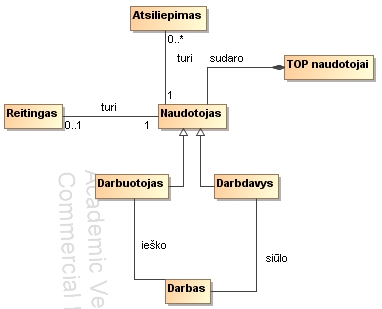
\includegraphics[scale=1, frame]{img/esybiu.png}
\caption{Esybių klasių diagrama}
\end{figure}
Esybių diagramoje (20 pav.) vaizduojamos esybių sąsajos. Pagrindinė esybė Naudotojas, kuris gali būti arba Darbuotojas, arba Darbdavys. Darbuotojas turi galimybę ieškoti, o darbdavys siūlyti darbą. Taip pat Naudotojas gali neturėti arba turėti reitingą  t.y. visų suteiktų reitingų vidurkį.  Dar vienas šios esybės privalumas yra neribotas skaičius atsiliepimų. TOP naudotojai yra sudaryti iš naudotojų atsižvelgiant į reikiamus kriterijus.
\subsubsection{Klasių diagrama (pirmas lygis)}
\begin{figure}[H]
\centering
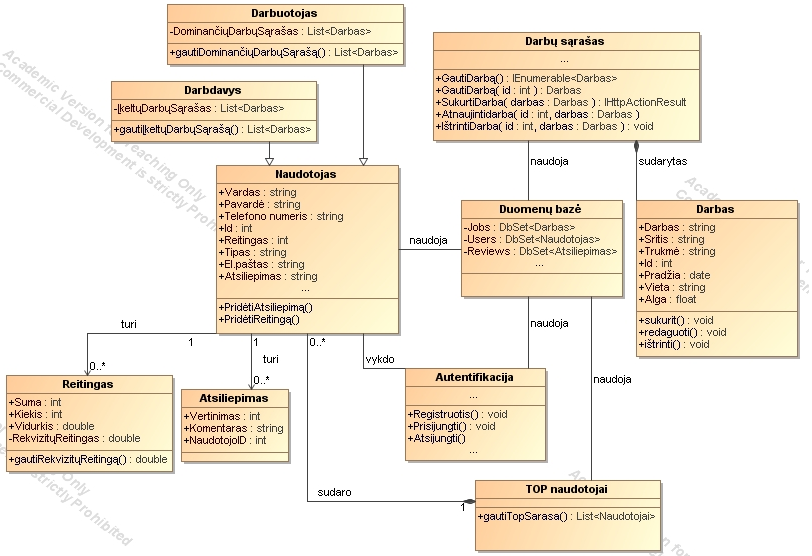
\includegraphics[width=\linewidth, frame]{img/klasiu.png}
\caption{Klasių diagrama}
\end{figure}
Pagrindinį programos funkcionalumą užtikrina šios klasės: Darbuotojas, Darbdavys, Naudotojas, TOP naudotojai, Reitingas, Atsiliepimas, Darbų sąrašas, Autentifikacija, Duomenų bazė, Darbas. Veikimą įgyvendinačių klasių tarpusavio bendradarbiavimas vaizduojamas asociacija, generalizacija, kompozicija bei  kardinalumus (21 pav.).
\newpage

%UŽDUOČIŲ PJŪVIS
\subsection{UŽDUOČIŲ PJŪVIS}
Šiame skyriuje aprašomas kuriamos sistemos galimi panaudojimo atvejai. Pasinaudojant užduočių diagrama  pateikiami darbdavio ir darbuotojo (Workly naudotojų) tikslai darbų valdymo sistemai.  Kiekvienai užduočiai pateikiamas scenarijus, kuris parodo, kaip užduotis įgyvendinama.
\subsubsection{Sistemoje vykdomos užduotys}
\begin{figure}[H]
\centering
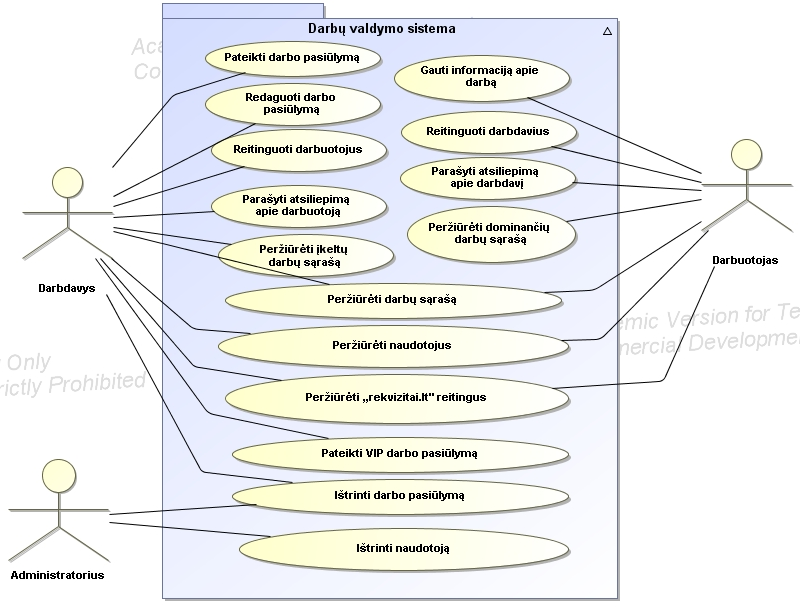
\includegraphics[width=\linewidth, frame]{img/usecase1.png}
\caption{Sistemoje vykdomos užduotys}
\end{figure}
Sistemoje vykdomos pagrindinės užduotys: darbuotojas siekia susirasti ieškomą darbą, reitinguoti darbdavius, peržiūtėti dominančius darbo pasiūlymus. Darbdavys siekia pateikti, redaguoti ar ištrinti darbo pasiūlymą, reitinguoti darbuotojus, peržiūrėti įkeltus darbus, parašyti VIP darbo pasiūlymą. Ir darbdavys, ir darbuotojas nori peržiūrėti darbų sąrašą, peržiūrėti TOP darbdavius ir darbuotojus, parašyti atsiliepimus.Administratorius gali ištrinti naudotoją ar darbo pasiūlymą. Šios užduotys leidžia vartotojui patogiai naudotis sistema ir išspręsti su darbais susijusius klausimus (22 pav.).
\newpage
\subsubsection{Užduočių vykdomo scenarijai}
Užduočių vykdymo scenarijai, atvaizduoja agentų, šiuo atveju darbdavio ir darbuotojo, įmanomų įvykdyti užduočių veiksmus paeiliui , nuo pradžios iki užduoties vykdymo pabaigos.
%
\subsubsubsection{Užduoties „Pateikti darbo pasiūlymą" scenarijus}
\begin{figure}[H]
\centering
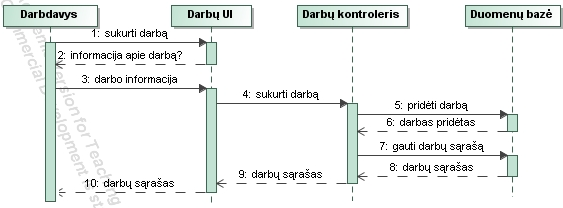
\includegraphics[scale=0.9, frame]{img/seku(pridetidarba).png}
\caption{Užduoties „Pateikti darbo pasiūlymą" scenarijus}
\end{figure}
	\textbf{Žingsnių seka (23 pav.):}\\
	1. Sukurti darbą - darbdavys paspaudžia ant nuorodos leidžiančios įkelti naują darbo pasiūlymą. \\
	2. Informacija apie darbą? - darbų UI išmeta darbdaviui darbo įkėlimo formą užpildymui. \\
	3. Darbo informacija - naudotojas išsiunčia užpildytą formą darbų UI. \\
	4. Sukurti darbą - įvesta darbo informacija yra siunčiama kontroleriui. \\
	5. Pridėti darbą - darbų UI įdeda darbą į duomenų bazę. \\
	6.Darbas pridėtas - duomenų bazė parsiunčia darbo patalpinimo patvirtinimą.\\
	7.Gauti darbų sąrašą - darbų kontroleris prašo duomenų bazės pateikti naują darbų sąrašą.\\
	8-10. Darbų sąrašas - darbų sąrašas keliauja iš duomenų bazės iki darbdavio. 
%
\subsubsubsection{Užduoties „Ištrinti darbo pasiūlymą" scenarijus}
\begin{figure}[H]
\centering
\includegraphics[width=\linewidth, frame]{img/seku(istrintidarba).png}
\caption{Užduoties „Ištrinti darbo pasiūlymą" scenarijus}
\end{figure}
	\textbf{Žingsnių seka (24 pav.):}\\
	1. Ištrinti darbą - darbdavys paspaudžia nuorodą ištrinančią darbo pasiūlymą. \\
	2. Ištrinti darbą? - naudotojas prašomas patvirtinti ištrynimą. \\
	3. Patvirtinti ištrynimą - darbdavys patvirtina ištrynimą. \\
	4. Patvirtintas darbo ištrynimas- pateikiamas darbas ištrynimui įvykdyti. \\
	5. Ištrinti darbą - prašoma duomenų bazės surasti ir ištrinti darbą.\\
	6. Gauti darbų sąrašą - siunčiamas prašymas darbų sąrašui gauti iš duomenų bazės. \\
	7-9. Darbų sąrašas - atnaujintas sąrašas keliauja iki darbdavio. 
%
\subsubsubsection{Užduoties „Redaguoti darbo pasiūlymą" scenarijus}
\begin{figure}[H]
\centering
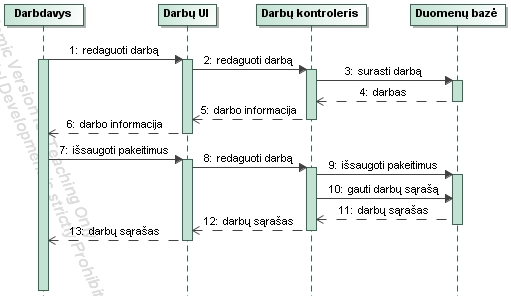
\includegraphics[width=\linewidth, frame]{img/seku(redaguotidarba).png}
\caption{Užduoties „Redaguoti darbo pasiūlymą" scenarijus}
\end{figure}
	\textbf{Žingsnių seka (25 pav.):}\\
	1. Redaguoti darbą - darbdavys paspaudžia nuorodą leidžiančią redaguoti darbą. \\
	2. Redaguoti darbą - pateikiamas darbas darbų kontroleriui.\\
	3. Surasti - darbas ieškomas duomenų bazėje.\\
	4. Darbas - duomenų bazė pateikia darbą kontroleriui.\\
	5-6. Darbo informacija - informacija apie darbą keliauja iki naudotojo.\\
	7. Išsaugoti pakeitimus - naudotojas prašo išsaugoti įvykdytus pakeitimus. \\
	8. Redaguoti darbą - darbas siunčiamas redagavimui. \\
	9. Išsaugoti pakeitimus – pakeitimai išsaugomi duomenų bazėje.\\
	10. Gauti darbų sąrašą – kontroleris prašo duomenų bazės gauti atnaujintą darbų sąrašą.\\
	11-13. Darbų sąrašas – darbų sąrašas keliauja iš duomenų bazės iki darbdavio.
%
\subsubsubsection{Užduoties „Peržiūrėti darbų sąrašą" scenarijus}
\begin{figure}[H]
\centering
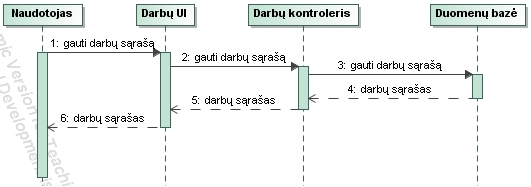
\includegraphics[width=\linewidth, frame]{img/seku(gautisarasa).png}
\caption{Užduoties „Peržiūrėti darbų sąrašą" scenarijus}
\end{figure}
	\textbf{Žingsnių seka (26 pav.):}\\
	1. Gauti darbų sąrašą -  naudotojas paspaudžia nuorodą į darbų sąrašą.\\
	2-3. Gauti darbų sąrašą– prašymas gauti darbų sąrašą keliauja iki duomenų bazės.\\
	4-6. Darbų sąrašas – darbų sąrašas iš duomenų bazės keliauja iki naudotojo.
%
\subsubsubsection{Užduoties „Reitinguoti darbuotojus" scenarijus}
\begin{figure}[H]
\centering
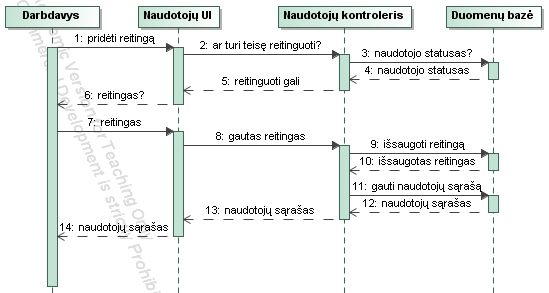
\includegraphics[width=\linewidth, frame]{img/seku(reitinguotidarbuotoja).png}
\caption{Užduoties „Retinguoti darbuotojus" scenarijus}
\end{figure}
	\textbf{Žingsnių seka (27 pav.):}\\
	1. Pridėti reitingą – darbdavys paspaudžia nuorodą leidžiančią pridėti reitingą.\\
	2. Ar turi teisę reitinguoti? – naudotojų UI siunčia kontroleriui užklausą reitingavimo patvirtinimui.\\
	3. Naudotojo statusas? – kontroleris siunčia duomenų bazei užklausą darbdavio statusui sužinoti.\\
	4. Naudotojo statusas – duomenų bazė parsiunčia darbdavio statusą.\\
	5. Reitinguoti gali – kontroleris patvirtina, kad reitinguoti galima.\\
	6. Reitingas? – naudotojų UI užklausia darbdavio reitingo.\\
	7. Reitingas – darbdavys pateikia reitingą.\\
	8. Gautas reitingas – naudotojų UI siunčia reitingą kontroleriui.\\
	9. Išsaugoti reitingą – reitingas siunčiamas į duomenų bazę išsaugojimui.\\
	10. Išsaugotas reitingas – parsiunčiamas reitingo išsaugojimo patvirtinimas.\\
	11. Gauti naudotojų sąrašą – kontroleris siunčia prašymą duomenų bazei naudotojų sąrašui gauti.\\
	12-14. Naudotojų sąrašas – naudotojų sąrašas iš duomenų bazės keliauja iki darbdavio.\\
%
\subsubsubsection{Užduoties „Reitinguoti darbdavius" scenarijus}
\begin{figure}[H]
\centering
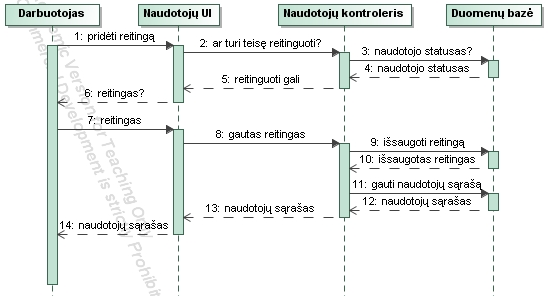
\includegraphics[width=\linewidth, frame]{img/seku(reitinguotidarbdavi).png}
\caption{Užduoties „Retinguoti darbdavius" scenarijus}
\end{figure}
	\textbf{Žingsnių seka (28 pav.):}\\
	1. Pridėti reitingą – darbuotojas paspaudžia nuorodą leidžiančią pridėti reitingą.\\
	2. Ar turi teisę reitinguoti? – naudotojų UI siunčia kontroleriui užklausą reitingavimo patvirtinimui.\\
	3. Naudotojo statusas? – kontroleris siunčia duomenų bazei užklausą darbuotojo statusui sužinoti.\\
	4. Naudotojo statusas – duomenų bazė parsiunčia darbuotojo statusą.\\
	5. Reitinguoti gali – kontroleris patvirtina, kad reitinguoti galima.\\
	6. Reitingas? – naudotojų UI užklausia darbuotojo reitingo.\\
	7. Reitingas – darbuotojas pateikia reitingą.\\
	8. Gautas reitingas – naudotojų UI siunčia reitingą kontroleriui.\\
	9. Išsaugoti reitingą – reitingas siunčiamas į duomenų bazę išsaugojimui.\\
	10. Išsaugotas reitingas – parsiunčiamas reitingo išsaugojimo patvirtinimas.\\
	11. Gauti naudotojų sąrašą – kontroleris siunčia prašymą duomenų bazei naudotojų sąrašui gauti.\\
	12-14. Naudotojų sąrašas – naudotojų sąrašas iš duomenų bazės keliauja iki darbuotojo.\\

%
\subsubsubsection{Užduoties „Parašyti atsiliepimą apie darbuotoją" scenarijus}
\begin{figure}[H]
\centering
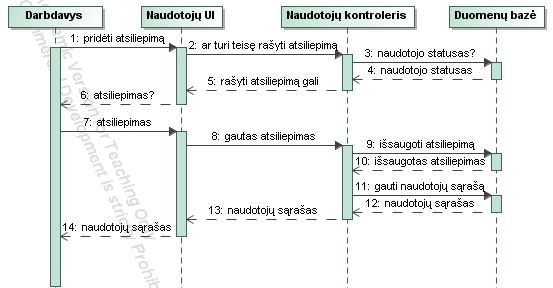
\includegraphics[width=\linewidth, frame]{img/seku(darbdavioatsiliepimas).png}
\caption{Užduoties „Parašyti atsiliepimą apie darbuotoją" scenarijus}
\end{figure}
	\textbf{Žingsnių seka (29 pav.):}\\
	1. Pridėti atsiliepimą – darbdavys paspaudžia nuorodą leidžiančią rašyti atsiliepimą.\\
	2. Ar turi teisę rašyti atsiliepimą? – naudotojų UI siunčia kontroleriui užklausą atsiliepimo rašymo patvirtinimui.\\
	3. Naudotojo statusas? – kontroleris siunčia duomenų bazei užklausą darbdavio statusui sužinoti.\\
	4. Naudotojo statusas – duomenų bazė parsiunčia darbuotojo statusą.\\
	5. Rašyti atsiliepimą gali – kontroleris patvirtina, kad rašyti atsiliepimą galima.\\
	6. Atsiliepimas? – naudotojų UI užklausia darbdavio atsiliepimo.\\
	7. Atsiliepimas– darbdavys pateikia atsiliepimą.\\
	8. Gautas atsiliepimas – naudotojų UI siunčia atsiliepimą kontroleriui.\\
	9. Išsaugoti atsiliepimą – atsiliepimas siunčiamas į duomenų bazę išsaugojimui.\\
	10. Išsaugotas atsiliepimas – parsiunčiamas atsiliepimo išsaugojimo patvirtinimas.\\
	11. Gauti naudotojų sąrašą – kontroleris siunčia prašymą duomenų bazei naudotojų sąrašui gauti.\\
	12-14 Naudotojų sąrašas – naudotojų sąrašas iš duomenų bazės keliauja iki darbdavio.\\
%
\subsubsubsection{Užduoties „Parašyti atsiliepimą apie darbdavį" scenarijus}
\begin{figure}[H]
\centering
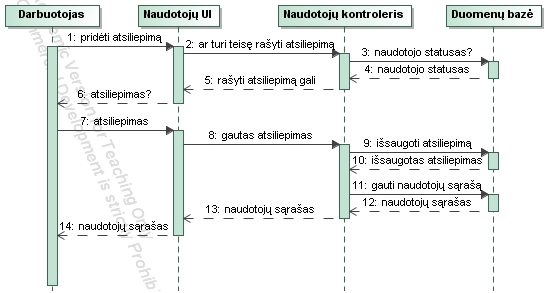
\includegraphics[width=\linewidth, frame]{img/seku(darbuotojoatsiliepimas).png}
\caption{Užduoties „Parašyti atsiliepimą apie darbdavį" scenarijus}
\end{figure}
	\textbf{Žingsnių seka (30 pav.):}\\
	1. Pridėti atsiliepimą – darbuotojas paspaudžia nuorodą leidžiančią rašyti atsiliepimą.\\
	2. Ar turi teisę rašyti atsiliepimą? – naudotojų UI siunčia kontroleriui užklausą atsiliepimo rašymo patvirtinimui.\\
	3. Naudotojo statusas? – kontroleris siunčia duomenų bazei užklausą darbuotojo statusui sužinoti.\\
	4. Naudotojo statusas – duomenų bazė parsiunčia darbuotojo statusą.\\
	5. Rašyti atsiliepimą gali – kontroleris patvirtina, kad rašyti atsiliepimą galima.\\
	6. Atsiliepimas? – naudotojų UI užklausia darbuotojo atsiliepimo.\\
	7. Atsiliepimas– darbuotojas pateikia atsiliepimą.\\
	8. Gautas atsiliepimas – naudotojų UI siunčia atsiliepimą kontroleriui.\\
	9. Išsaugoti atsiliepimą – atsiliepimas siunčiamas į duomenų bazę išsaugojimui.\\
	10. Išsaugotas atsiliepimas – parsiunčiamas atsiliepimo išsaugojimo patvirtinimas.\\
	11. Gauti naudotojų sąrašą – kontroleris siunčia prašymą duomenų bazei naudotojų sąrašui gauti.\\
	12-14. Naudotojų sąrašas – naudotojų sąrašas iš duomenų bazės keliauja iki darbuotojo.\\
%
\subsubsubsection{Užduoties „Gauti informaciją apie darbą" scenarijus}
\begin{figure}[H]
\centering
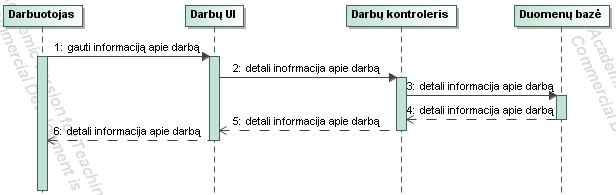
\includegraphics[width=\linewidth, frame]{img/seku(gautiinformacija).png}
\caption{Užduoties „Gauti informaciją apie darbąį" scenarijus}
\end{figure}
	\textbf{Žingsnių seka (31 pav.):}\\
	1. Gauti informaciją apie darbą – darbuotojas paspaudžia ant nuorodos informacijai apie darbą gauti.\\
	2–3. Detali informacija apie darbą – darbų UI siunčia prašymą kontroleriui, kuris siunčia prašymą duomenų bazei, pateikti detalią informaciją apie darbą.\\
	4– 6. Detali informacija apie darbą – iš duomenų bazės informacija keliauja iki darbuotojo.\\
%
\subsubsubsection{Užduoties „Gauti naudotojų sąrašą" scenarijus}
\begin{figure}[H]
\centering
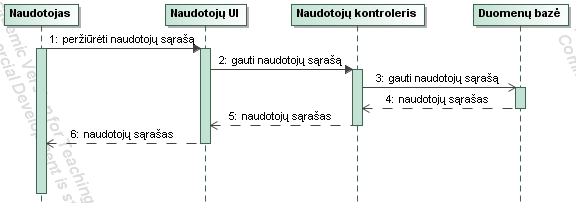
\includegraphics[width=\linewidth, frame]{img/seku(naudotojusarasas).png}
\caption{Užduoties „Gauti naudotojų sąrašąį" scenarijus}
\end{figure}
	\textbf{Žingsnių seka (32 pav.):}\\
	1. Peržiūrėti naudotojų sąrašą – naudotojas spaudžia nuorodą nukreipiančią į naudotojų sąrašą.\\
	2–3. Gauti naudotojų sąrašą – prašymas gauti naudotojų sąrašą keliauja nuo naudotojų UI iki duomenų bazės.\\
	4–6. Naudotojų sąrašas – iš duomenų bazės naudotojų sąrašas keliauja iki pat naudotojo.\\
%
\subsubsubsection{Užduoties „Gauti dominančių darbų sąrašą" scenarijus}
\begin{figure}[H]
\centering
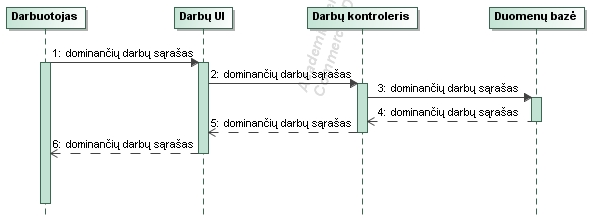
\includegraphics[width=\linewidth, frame]{img/seku(dominantys).png}
\caption{Užduoties „Gauti dominančių darbų sąrašą" scenarijus}
\end{figure}
	\textbf{Žingsnių seka (33 pav.):}\\
	1-3. Dominančių darbų sąrašas – nuo darbuotojo nuorodos paspaudimo iki duomenų bazės keliauja užklausa dominančių darbų sąrašui gauti.\\
	4–6. Dominančių darbų sąrašas – iš duomenų bazės dominančių darbų sąrašas keliauja iki darbuotojo.\\
\subsubsubsection{Užduoties „Gauti įkeltų darbų sąrašą" scenarijus}
\begin{figure}[H]
\centering
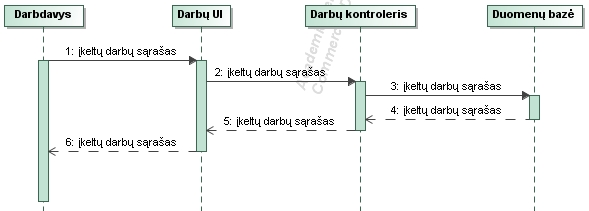
\includegraphics[width=\linewidth, frame]{img/seku(ikelti).png}
\caption{Užduoties „Gauti įkeltų darbų sąrašą" scenarijus}
\end{figure}
	\textbf{Žingsnių seka (34 pav.):}\\
	1-3. Įkeltų darbų sąrašas – nuo darbdavio nuorodos paspaudimo iki duomenų bazės keliauja užklausa įkeltų darbų sąrašui gauti.\\
	4-6. Įkeltų darbų sąrašas – įkeltų darbų sąrašas, rastas duomenų bazėje, keliauja iki darbdavio.\\
\newpage
%KūRIMO PJŪVIS
\subsection{KŪRIMO PJŪVIS}
Programų sistemos komponentai yra vaizduojami trimis lygmenimis: nuliniu, pirmuoju, antruoju. Toks komponentų pateikimas leidžia išsamiau apibrėžti sistemos fizinius komponentus, jų konfigūraciją bei tarpusavio sąryšius. Komponentų diagramos atvaizduodamos struktūrą, komponentų priklausomybes bei sąsajas leidžia susidaryti sistemos fizinį vaizdą. Taip pat suteikia galimybę apžvelgti išoriškai matomą komponentų elgseną. Komponentai atvaizduojami naudojant UML komponentų diagramas.
\subsubsection{Komponentų diagramos nulinis lygmuo}
\begin{figure}[H]
\centering
\includegraphics[width=\linewidth, frame]{img/komponentu0.png}
\caption{Komponentų diagramos nulinis lygmuo}
\end{figure}
Komponentų diagramos nuliniame lygmenyje (35 pav.) vaizduojamas bendras komponentų vaizdas. Pagrindinis ir vienintelis šio lygio komponentas yra „Darbų valdymo sistema“. Šis komponentas sąveikauja su įvairiais interfeisais. Darbdavio ir darbuotojo UI parodo paslaugas, kurias pagrindinis komponentas siūlo savo aplinkai, šiuo atveju komponentas paduoda grafinį interfeisą, kuriuo gali naudotis darbuotojas ir darbdavys.
\subsubsection{Komponentų diagramos pirmas lygmuo}
\begin{figure}[H]
\centering
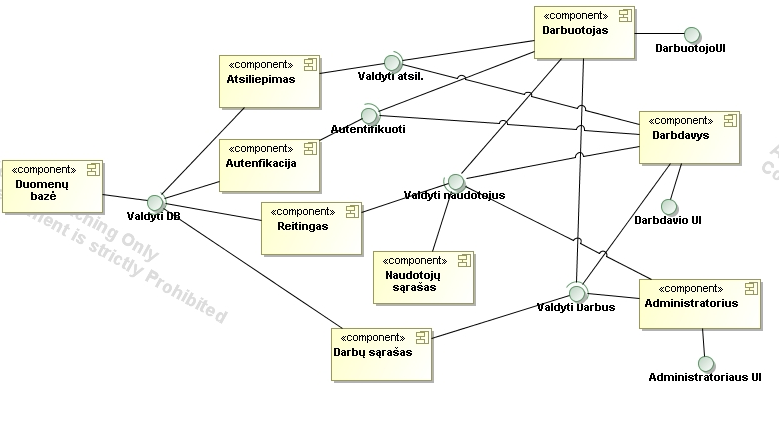
\includegraphics[width=\linewidth, frame]{img/komponentu2.png}
\caption{Komponentų diagramos pirmas lygmuo}
\end{figure}
Komponentų diagramos pirmame lygmenyje (36 pav.) lygyje komponentų diagrama yra suskaidoma. Darbų valdymo sistemos komponentas yra dekomponuojamas į DB, Atsiliepimas, Autentifikacija, Reitingas, TOP‘ai, Darbų sąrašas, Darbuotojas, Darbdavys komponentus. Šiame lygyje visi interfeisai turi už juos atsakingus tam tikrus komponentus. Kiekvienas komponentas tiekia sąsajas, kad kiti komponentai galėtų sąveikauti ir gauti komponento teikiamas paslaugas. Tokiu būdu yra užtikrinama pilna komponentų realizacija bei savitarpio darna. 
Komponentai yra išdėstyti ir pavaizduoti tokiu būdu, nes tai geriausiai atspindi mūsų sistemos vizijos funkcionalumą. 
\subsubsection{Komponentų diagramos antras lygmuo}
\begin{figure}[H]
\centering
\includegraphics[scale=1, frame]{img/komponentu3.png}
\caption{Komponentų diagramos antras lygmuo}
\end{figure}
Komponentų diagramos pirmame lygmenyje (37 pav.) komponentų diagrama yra dar detaliau suskaidoma. Dekomponavimui pasitelkiamas MVC dizaino šablonas, kuris leidžia įgyvendinti naudotojo interfeisą. Šis modelis buvo pasirinktas, nes yra dažnai naudojamas ir populiarus . Trys pagrindiniai komponentai sudaro MVC: Model, View ir Controller. Model – pagrindinis šablono komponentas, jis atsakingas už sistemos elgesį probleminėje situacijoje, nepriklausomai nuo vartotojo sąsajos, taip pat jis atsakingas už duomenis, logiką ir taisykles. View – komponentas, kuris yra atsakingas už diagramų, lentelių bei kitos informacijos vaizdavimą. Cotroller – komponentas, kuris rūpinasi duomenų įvestimi ir įvesties konvertavimu.
\newpage
%FIZNIS PJŪVIS
\subsection{FIZINIS PJŪVIS}
Fizinis pjūvis sudarytas iš dislokavimo diagramų. Šiose diagramose vaizduojamas programos komponentų išdėstymas tinkle bei komunikacijos protokolai tarp jų. Tuo pačiu diagramose parodoma, kokia programinė įranga turi būti įdiegta fiziniuose sistemos komponentuose.
\subsubsection{Dislokavimo diagrama nr.1 (komponentų ir artefaktų ryšių diagrama)}
\begin{figure}[H]
\centering
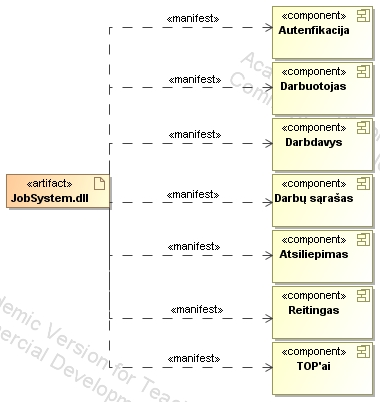
\includegraphics[scale=0.8, frame]{img/fizinis(artefaktai).png}
\caption{Komponentų ir artifaktų ryšių diagrama}
\end{figure}
Komponentų ir artefaktų ryšių diagramoje (38 pav.) vaizduojamas artefaktas JobSystem.dll, kuris įgyvendina šiuos programos komponentus: Autentifikacija, Darbuotojas, Darbdavys, Darbų sąrašas, Atsiliepimas, Reitingas, TOP’ai.
\subsubsection{Dislokavimo diagrama nr.2 (mazgų ir artefaktų ryšių diagrama)}
\begin{figure}[H]
\centering
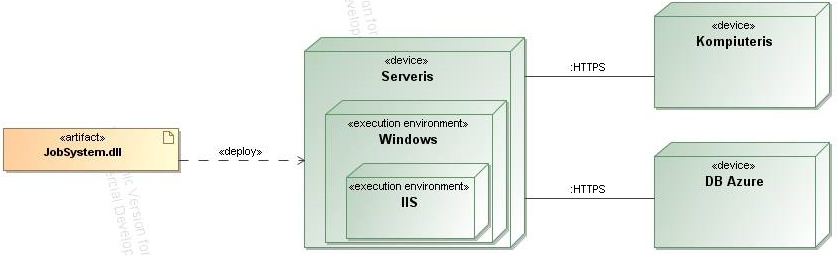
\includegraphics[width=\linewidth, frame]{img/fizinis2.png}
\caption{Mazgų ir artifaktų ryšių diagrama}
\end{figure}
Mazgų ir artefaktų diagramoje (39 pav.) parodoma, kad tinkle artefaktas JobSystem.dll yra įdiegtas Windows operacinės sistemos serveryje ir veikia IIS aplinkoje. Ši programinė įranga yra pasirinkta dėl programos naudojamo ASP.NET MVC šablono reikalavimų. Serveris taip pat bendrauja http protokolu su AZURE SQL serveriu, kuriame saugoma programos duomenų bazė. Klientai turi galimybe pasiekti sistemos teikiamas paslaugas savo pasirinkta naršykle, kuri palaiko http protokolą.
\subsubsection{Dislokavimo diagrama nr.3 (mazgų ir artefaktų egzempliorių diagrama)}
\begin{figure}[H]
\centering
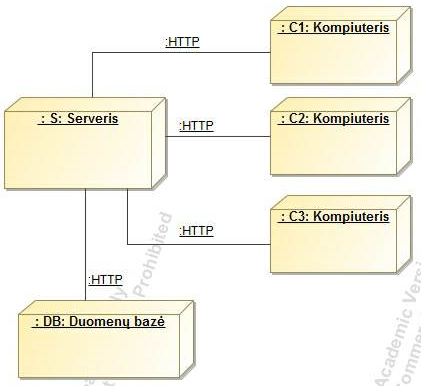
\includegraphics[scale=1, frame]{img/fizinis3.png}
\caption{Mazgų ir artifaktų ryšių diagrama}
\end{figure}
40 pav. vaizduojamas įrenginių (mazgų) išsidėstymas tinkle.  Serveris turi tiesioginį ryšį su duomenų baze, o vartotojai gali prisijungti prie serverio. Tačiau klientai negali tiesiogiai pasiekti duomenų bazės ir joje saugomų duomenų.
\newpage

%PROCESO PJŪVIS
\subsection{PROCESO PJŪVIS}
Procesų pjūvis sudarytas iš sekų ir veiklos diagramų. Diagramose parodoma, kokie procesai vyksta sistemoje. Taip pat išreiškiama komunikacija tarp jų. Tikrinama, ar komunikacijos nėra per daug. 
%%%%%
\subsubsection{Proceso sekų diagramos}
Procesų sekų diagramose, atsispindi procesai, kurie yra vykdomi sistemoje. Iš proceso sekų diagramos galima matyti, kokie komponentai dalyvauja vykdyme, kaip procesas vykdomas.
\subsubsection{Proceso „Prisijungimas" sekų diagrama}
\begin{figure}[H]
\centering
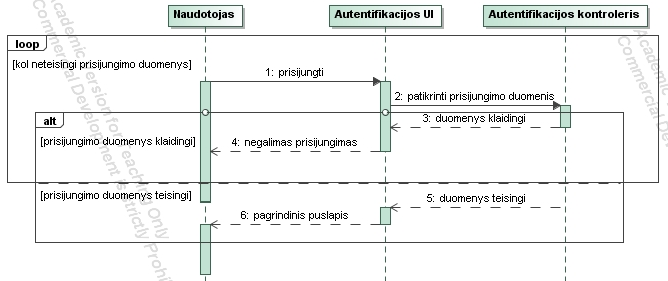
\includegraphics[width=\linewidth, frame]{img/proceso(prisijungimas).png}
\caption{Proceso „Prisijungimas" sekų diagrama}
\end{figure}
Procesas prasideda naudotojo paspaudimu ant nuorodos įgalinančios prisijungimą. Autentifikacijos UI gautus duomenis siunčia patikrinimui į autentifikacijos kontrolerį. Iš kontrolerio gaunamas atsakymas, ar duomenys teisingi ar ne. Jei duomenys klaidingi, vartotojui išmetamas pranešimas, jog prisijungti negalima ir jis vėl gali kartoti prisijungimo procesą. Jei duomenys teisingi, naudotojas yra nukreipiamas į pagrindinį puslapį (41 pav.).
\subsubsection{Veiklos diagramos}
Šiame skyriuje pateikiamos veiklos diagramos. Jos padeda suprasti dinaminį sistemos veikimą, parodo, kokie veiksmai atliekami vykdant konkrečią veiklą, galimus vykdymo atvejus.
\subsubsubsection{Registracijos veiklos diagrama}
\begin{figure}[H]
\centering
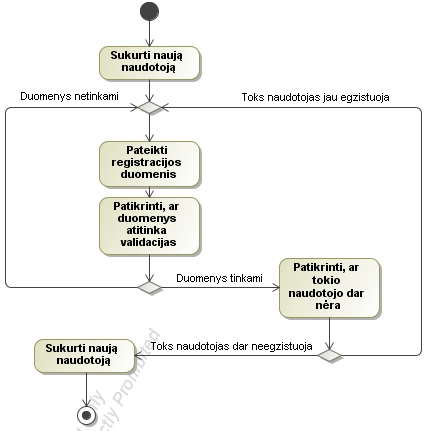
\includegraphics[scale=1, frame]{img/veiklos(registracija).png}
\caption{Registracijos veiklos diagrama}
\end{figure}
Diagramoje vaizduojamas naudotojo užsiregistravimas sistemoje. Procesas prasideda vartotojo nuorodos paspaudimu, kreipiančios į registravimo formą. Naudotojas pateikia visus reikiamus duomenis, tuomet, jie siunčiami patikrinimui. Jei duomenys netinkami, naudotojas nukreipiamas atgal į registravimo formą. Jei duomenys atitinka visus reikalavimus, tai siunčiami toliau patikrinimui, ar toks naudotojas dar neegzistuoja. Jei egzistuoja, tai naudotojas nukreipiamas atgal į registravimo formą. Jei dar tokio naudotojo nėra sistemoje, yra sukuriamas naujas naudotojas ir veikla nutraukiama (42 pav.)
\subsubsubsection{Darbo pridėjimo veiklos diagrama}
\begin{figure}[H]
\centering
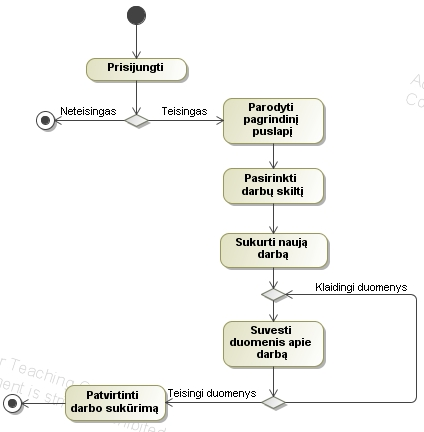
\includegraphics[scale=1, frame]{img/veiklos(pridetiDarba).png}
\caption{Darbo pridėjimo veiklos diagrama}
\end{figure}
Diagramoje (43 pav.) vaizduojamas naudotojo naujo darbo patalpinimas sistemoje. Procesas prasideda nuo prisijungimo. Jei prisijungimas neteisingas, visos veiklos yra sustabdomos. Jei prisijungiama sėkmingai, naudotojui parodomas pagrindinis puslapis, kuriame jis gali pasirinkti darbų skiltį. Tuomet, prisijungęs vartotojas gali sukurti naują darbą paspausdamas nuorodą. Sistema išmetą darbo formą, kurioje naudotojas turi suvesti duomenis. Jei duomenys klaidingi, grįžtama atgal į darbo formą. Jei duomenys teisingi, naudotojui telieka patvirtinti darbo sukūrimą ir procesas yra pabaigiamas.
\newpage
\subsection{RYŠIAI TARP PJŪVIŲ}
Šiame skyriuje pateikiama, kaip vieni pjūviai yra susiję su kitais. Tam naudojamos matricos.
\subsubsection{Užduočių ir kūrimo pjūvių ryšių matrica}
\begin{figure}[H]
\centering
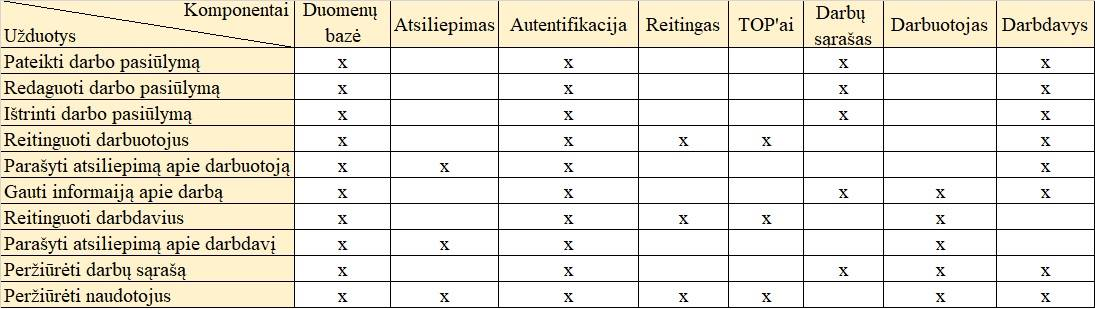
\includegraphics[width=\linewidth, frame]{img/matricaUK.jpg}
\caption{Užduočių ir kūrimo pjūvių ryšių matrica}
\end{figure}
44 pav. matricoje vaizduojama, kokie komponentai dalyvauja užduoties atlikime.
\subsubsection{Loginio ir kūrimo pjūvių ryšių matrica}
\begin{figure}[H]
\centering
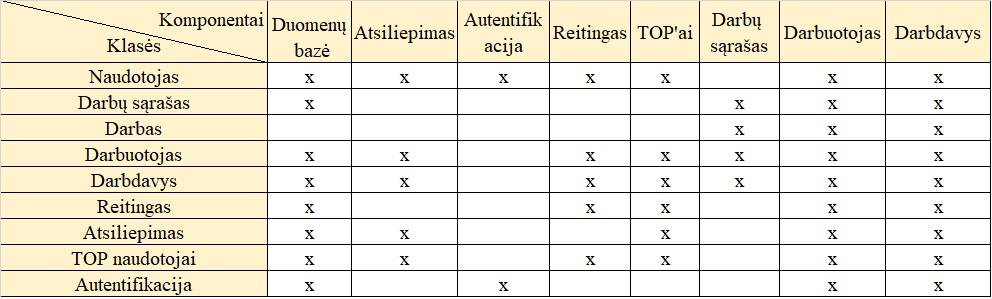
\includegraphics[width=\linewidth, frame]{img/matricaLK.jpg}
\caption{Loginio ir kūrimo pjūvių ryšių matrica}
\end{figure}
45 pav. matricoje vaizduojama kokiems komponentams priklauso klasės. Matrica leidžia patikrinti, ar visos esybės/klasės yra įgyvendintos.

\sectionnonum{1 priedas. Sistemos prototipai}
1 priede vaizduojami sistemos grafinio vaizdo prototipai. Tai yra eskizai sistemos įsivaizdavimui. 46-65 pav.)
\begin{figure}[H]
\centering
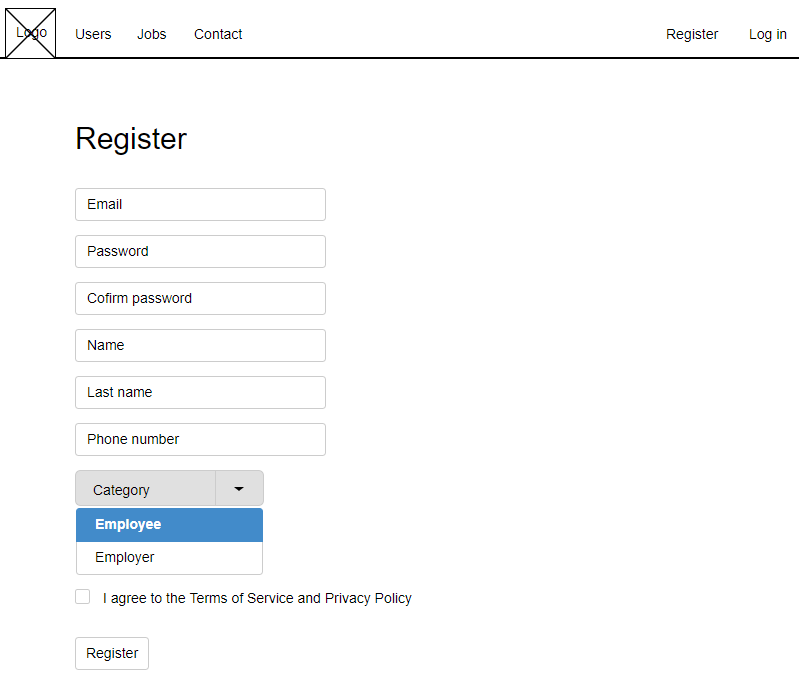
\includegraphics[width=\linewidth, frame]{img/registerForm.png}
\caption{Registracijos forma}
\end{figure}

\begin{figure}[H]
\centering
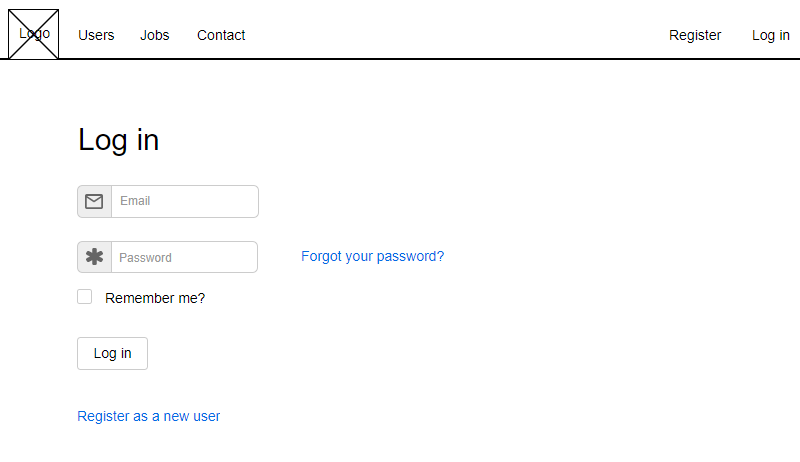
\includegraphics[width=\linewidth, frame]{img/logInForm.png}
\caption{Prisijungimo forma}
\end{figure}

\begin{figure}[H]
\centering
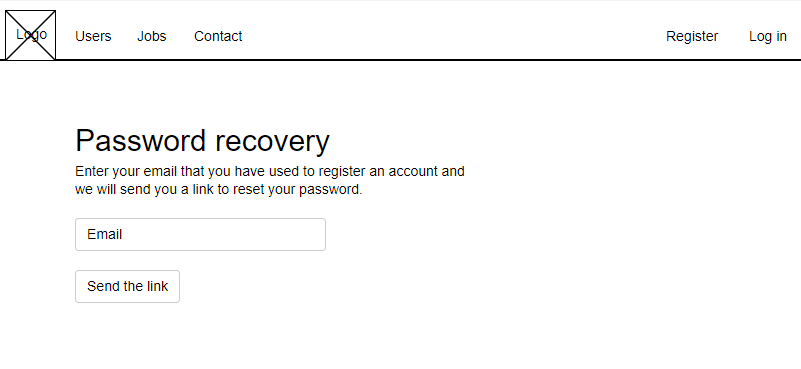
\includegraphics[width=\linewidth, frame]{img/passwordRecovery.png}
\caption{Slaptažodžio priminimo forma}
\end{figure}

\begin{figure}[H]
\centering
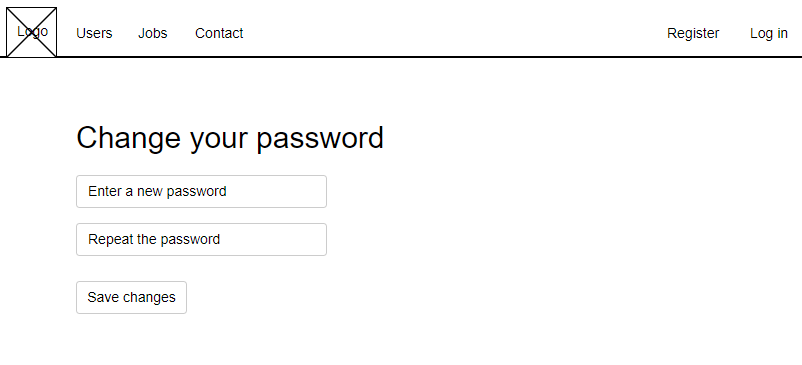
\includegraphics[width=\linewidth, frame]{img/passReset.png}
\caption{Slaptažodžio pakeitimo forma}
\end{figure}

\begin{figure}[H]
\centering

\includegraphics[width=\linewidth, frame]{img/contact.png}
\caption{Kontaktų puslapis}
\end{figure}

\begin{figure}[H]
\centering
\includegraphics[width=\linewidth, frame]{img/employeeHomePage.png}
\caption{Pagrindinis puslapis iš darbdavio perspektyvos.}
\end{figure}

\begin{figure}[H]
\centering
\includegraphics[width=\linewidth, frame]{img/guestHomePage.png}
\caption{Pagrindinis puslapis iš neprisijungusio naudotojo perspektyvos.}
\end{figure}

\begin{figure}[H]
\centering
\includegraphics[width=\linewidth, frame]{img/employeeHomePage.png}
\caption{Pagrindinis puslapis iš darbuotojo perspektyvos.}
\end{figure}

\begin{figure}[H]
\centering
\includegraphics[width=\linewidth, frame]{img/top.png}
\caption{Darbdavių ir darbuotojų sąrašai}
\end{figure}

\begin{figure}[H]
\centering
\includegraphics[width=\linewidth, frame]{img/employeeInfo.png}
\caption{Infromacijos apie darbuotoją puslapis}
\end{figure}

\begin{figure}[H]
\centering
\includegraphics[width=\linewidth, frame]{img/employerInfo.png}
\caption{Infromacijos apie darbdavį puslapis}
\end{figure}

\begin{figure}[H]
\centering
\includegraphics[width=\linewidth, frame]{img/employerJobs.png}
\caption{Darbo pasiūlymų sąrašas iš darbdavio perspektyvos.}
\end{figure}

\begin{figure}[H]
\centering
\includegraphics[width=\linewidth, frame]{img/employeeJobs.png}
\caption{Darbo pasiūlymų sąrašas iš darbuotojo perspektyvos.}
\end{figure}

\begin{figure}[H]
\centering
\includegraphics[width=\linewidth, frame]{img/jobInfo.png}
\caption{Informacjos apie darbą puslapis}
\end{figure}


\begin{figure}[H]
\centering
\includegraphics[width=\linewidth, frame]{img/interestedJobs.png}
\caption{Dominančių darbų sąrašo eskizas.}
\end{figure}


\begin{figure}[H]
\centering
\includegraphics[width=\linewidth, frame]{img/yourJobs.png}
\caption{Įkeltų darbo pasiūlymų sąrašo eskizas.}
\end{figure}

\begin{figure}[H]
\centering
\includegraphics[width=\linewidth, frame]{img/editJob.png}
\caption{Redaguoti darbo pasiūlymą.}
\end{figure}

\begin{figure}[H]
\centering
\includegraphics[width=\linewidth, frame]{img/createJob.png}
\caption{Darbo pasiūlymo įkėlimo forma.}
\end{figure}

\begin{figure}[H]
\centering
\includegraphics[width=\linewidth, frame]{img/myProfile.jpg}
\caption{Profilio puslapis.}
\end{figure}

\begin{figure}[H]
\centering
\includegraphics[width=\linewidth, frame]{img/changePass.png}
\caption{Slaptažodžio pakeitimo forma.}
\end{figure}

\sectionnonum{ŽODYNAS}
Šiame skyriuje pateikiami specifiniai mūsų projekte naudotų žodžių paaiškinimai.\\
\textbf{Sistema} – darbų valdymo sistema, dokumente vadinama „Workly“. \\
\textbf{Naudotojas} – asmuo, kuris naudojasi sistema. Naudotojas gali būti darbdavys, darbuotojas ir administratorius.\\
\textbf{Darbuotojas} – naudotojas, sistemoje ieškantis darbo.\\
\textbf{Darbdavys} – naudotojas, sistemoje pateikiantis darbų pasiūlymus.\\
\textbf{Darbas} – smulki veikla už atlygį, pasižyminti įvairiais kriterijais,  kurią darbdavys patalpina sistemoje. \\
\textbf{Darbų sąrašas} – visų sistemoje patalpintų darbų sąrašas.\\
\textbf{Atsiliepimas} – komentaras, kurį gali palikti darbuotojas darbdaviui ir atvirkščiai.\\
\textbf{Reitingas} – skaitinis įvertinimas, kurį darbuotojas palieka darbdaviui ir atvirkščiai. Taip pat reitingu yra laikomas  visų suteiktų naudotojui reitingų vidurkis.\\
\textbf{TOP‘ai} – geriausiai išreitinguotų darbuotojų ir darbdavių sąrašai. \\
\textbf{Hostingas} - svetainės talpinimas.\\
\textbf{AZURE} – Microsoft teikiama paslauga serverių nuomai ir jų valdymui.\\
\textbf{MS} - Microsoft.\\
\textbf{MSSQL} - atviro kodo reliacinių duomenų bazių valdymo sistema.\\
\textbf{Reliacinė duomenų bazė} - tai tokia duomenų visuma kurioje informacija saugoma dvimatėse lentelėse.\\
\textbf{IIS (Internet Information Services)}- serverio programinė įranga, sukurta Microsoft ir skirta veikti Windows NT šeimos operacinėse sistemose.\\
\textbf{Duomenų bazė} – darbų valdymo sistemos duomenų bazė, kurioje laikomas darbų, naudotojų bei TOP‘ų sąrašai, atsiliepimų ir reitingų duomenys.\\
\textbf{Artefaktas} – programos sukurtas informacijos vienetas.\\
\textbf{AZURE} – Microsoft teikiama paslauga serverių nuomai ir jų valdymui.\\
\sectionnonum{IŠVADOS}
Pateikta išorinė ir vidinė analizė, įgyvendinamumo ir naudos analizė padeda nustatyti, ar kuriama sistema yra paklausi rinkoje, kokios yra pagrindinės techininės kliūtys ir ar finansiškai apsimoka kurti tokią sistemą. Reikalavimų surinkimas padeda geriau įsivaizduoti kuriamą sistemą. Šis dokumentas bus pagrindas projektuotojams projektuojant sistemą, taip pat padės sukurti būtent tai, ko iš sistemos tikimasi. Taip pat tai padės įvertinti, ar sistema sudaryta gerai, ar atitinka užsakovo lūkesčius. Programos projektavimas užtikrina efektyvesnį programos vystimo procesą, suteikia lankstumo, plečiamumo galimybių. Pagal sukurtą sistemą parengus dokumentaciją, galima įsitikinti, kad programa yra įgyvendinama ir esminių trūkumų jos funkcionalume nėra.
\sectionnonum{ŠALTINIAI}
\begin{enumerate}
	\item  dr. Vytautas Valaitis internetinis puslapis (https://klevas.mif.vu.lt/~valaitis/)
	\item doc., dr. Karolio Petrausko iternetinis puslapis (http://klevas.mif.vu.lt/~karolis/)
\end{enumerate}
\end{document}
